\documentclass[
	% -- opções da classe memoir --
	12pt,				% tamanho da fonte
	openright,			% capítulos começam em pág ímpar (insere página vazia caso preciso)
	oneside,			% para impressão em verso e anverso. Oposto a oneside
	a4paper,			% tamanho do papel. 
	% -- opções da classe abntex2 --
	%chapter=TITLE,		% títulos de capítulos convertidos em letras maiúsculas
	%section=TITLE,		% títulos de seções convertidos em letras maiúsculas
	%subsection=TITLE,	% títulos de subseções convertidos em letras maiúsculas
	%subsubsection=TITLE,% títulos de subsubseções convertidos em letras maiúsculas
	% -- opções do pacote babel --
	english,			% idioma adicional para hifenização
	french,				% idioma adicional para hifenização
	spanish,			% idioma adicional para hifenização
	brazil				% o último idioma é o principal do documento
	dvipsnames, table]{abntex2}
\usepackage{graphicx} % Required for inserting images
\usepackage{xcolor}
\usepackage{longtable}
% \usepackage{subfigure}
\usepackage{float}
\usepackage{subfig}
\usepackage{url}

\usepackage{glossaries}
\makeglossaries
\newacronym{GFS}{GFS}{Global Forecast System}
\newacronym{MERRA2}{MERRA2}{Modern-Era Retrospective analysis for Research and Applications, Version 2}
\newacronym{MERGE}{MERGE}{Merging Technique}
\newacronym{SAMeT}{SAMeT}{South American Mapping of Temperature}
\newacronym{IBGE}{IBGE}{Instituto Brasileiro de Geografia e Estatística}
\newacronym{TRMM-TMPA}{TRMM-TMPA}{Tropical Rainfall Measuring Mission Multi-satellite Precipitation Analysis}
\newacronym{GPM-IMERG}{GPM-IMERG}{Integrated Multi-satellitE Retrievals for Global Precipitation Measurement}
\newacronym{ERA5}{ERA5}{ECMWF Reanalysis 5th Generation}
\newacronym{ECMWF}{ECMWF}{European Centre for Medium-Range Weather Forecasts}
\newacronym{GTOPO30}{GTOPO30}{Global Digital Elevation}
\newacronym{PCAM}{PCAM}{Programa de Pós-Graduação Mestrado Profissional em Clima e Ambiente}
\newacronym{PTT}{PTT}{Produto Técnico-Tecnológico}
\newacronym{FF}{FF}{Frentes Frias}
\newacronym{LI}{LI}{Linhas de Instabilidade}
\newacronym{CCM}{CCM}{Complexos Convectivos de Mesoescala}
\newacronym{ZCAS}{ZCAS}{Zona de Convergência do Atlântico Sul}
\newacronym{CDO}{CDO}{Climate Data Operators}
\newacronym{GrADS}{GrADS}{Grid Analysis and Display System}
\newacronym{GTS}{GTS}{Global Telecommunications System}
\newacronym{CPTEC}{CPTEC}{Centro de Previsão de Tempo e Estudos Climáticos}
\newacronym{INPE}{INPE}{Instituto Nacional de Pesquisas Espaciais}
\newacronym{MEC}{MEC}{Ministério da Educação}
\newacronym{CNPq}{CNPq}{Conselho Nacional de Desenvolvimento Científico e Tecnológico}
\newacronym{CAPES}{CAPES}{Coordenaçao de Aperfeiçoamento de Pessoal de Nível Superior}
\newacronym{ASOS}{ASOS}{Automatic Surface Observation Station}
\newacronym{OMS}{OMS}{Organização Mundial de Saúde}
\newacronym{ONU}{ONU}{Organização das Nações Unidas}
\newacronym{FAO}{FAO}{Organização das Nações Unidas para a Alimentação e a Agricultura}
\newacronym{CFMV}{CFMV}{Conselho Federal de Medicina Veterinária}
\newacronym{CRMV}{CRMV}{Conselho Regional de Medicina Veterinária}
\newacronym{SC}{SC}{Santa Catarina}
\newacronym{PR}{PR}{Paraná}
\newacronym{CEGRADE}{CEGRADE}{Comissão Estadual de Gestão de Riscos de Animais em Desastres}
\newacronym{Cobrade}{Cobrade}{Classificação e Codificação Brasileira de Desastres}
\newacronym{DF}{DF}{Distrito Federal}
\newacronym{PNCD}{PNCD}{Programa Nacional de Controle da Dengue}
\newacronym{DENV}{DENV}{Dengue Virus}
\newacronym{Funasa}{Funasa}{Fundação Nacional de Saúde}
\newacronym{ESRI}{ESRI}{Environmental Systems Research Institute}
\newacronym{DataSUS}{DataSUS}{Departamento de Informática do Sistema Único de Saúde}
\newacronym{Dive}{Dive}{Diretoria de Vigilância Epidemiológica}
\newacronym{LACEN}{LACEN}{Laboratório Central de Saúde Pública}
%\newacronym{DENV}{DENV}{vírus da dengue}
\newacronym{ssRNA}{ssRNA}{single-stranded Ribonucleic Acid}
\newacronym{ITIS}{ITIS}{Integrated Taxonomic Information System}
\newacronym{IFSC}{IFSC}{Instituto Federal de Ensino, Ciência e Tecnologia de Santa Catarina}
\newacronym{UFSM}{UFSM}{Universidade Federal de Santa Maria}
\newacronym{ESBMet}{ESBMet}{Encontro Sul Brasileiro de Meteorologia}
%\newacronym{PCAM}{PCAM}{Programa de Pós-graduação em Clima e Ambiente}
\newacronym{DEE}{DEE}{Dados Entomo-Epidemiológicos}
\newacronym{DEC}{DEC}{Dados de Elementos Climáticos}
\newacronym{DSG}{DSG}{Dados Socioeconômicos e Geográficos}
\newacronym{DGR}{DGR}{Dados Georreferenciados}
\newacronym{ICOb}{ICOb}{Índice Combinado por Observação}
\newacronym{ICRe}{ICRe}{Índices Corrigidos por Região}
\newacronym{LACOb}{LACOb}{Limiar de Alta Correlação Observado}
\newacronym{LACRe}{LACRe}{Limiares de Alta Correlação Regionalizados}
\newacronym{SBP}{SBP}{Sociedade Brasileira Técnico-Científica de Parasitologia}
\newacronym{JBN}{JBN}{Jatos de Baixos Níveis}
\newacronym{Bdmep/Inmet}{Bdmep/Inmet}{Banco de Dados Meteorológicos do Instituto Nacional de Meteorologia}
\newacronym{Inmet}{Inmet}{Instituto Nacional de Meteorologia}
\newacronym{CRS}{CRS}{Coordinate Reference System}
\newacronym{MAPA}{MAPA}{Ministério da Agricultura, Pecuária e Abastecimento}
\newacronym{Sinan}{Sinan}{Sistema de Informação de Agravos de Notificação}
\newacronym{Cenepi}{Cenepi}{Centro Nacional de Epidemiologia}
\newacronym{SVS}{SVS}{Secretaria de Vigilância em Saúde}
\newacronym{csv}{csv}{comma separated values}
\newacronym{nc}{NetCDF4}{Network Common Data Form version 4}
\newacronym{grib}{GRIB2}{Gridded Binary version 2}
\newacronym{ReLU}{ReLU}{Rectified Linear Unit}
\newacronym{RQEQM}{RQEQM}{Raiz Quadrada do Erro Quadrático Médio}
\newacronym{EMA}{EMA}{Erro Médio Absoluto}
\newacronym{r2}{R²}{Coeficiente de Determinação}
\newacronym{r}{r}{Coeficiente de Correlação}


\title{4_resultados_rascunho}
\author{Matheus Ferreira de Souza}
\date{July 2024}

\begin{document}

\maketitle

\newpage

\chapter{Apresentação dos Resultados}

\section{Análise e discussão dos resultados}

\indent Como forma de otimizar a leitura, os resultados serão apresentados e discutidos na sequência. Também como facilitação, a ordem e numeração apresentados seguirão os mesmos adotados na metodologia. Para analisar de forma mais detalhada, os resultados se encontram no \href{https://github.com/matheusf30/dengue/tree/main/resultados}{GitHub}, publicados no endereço eletrônico abaixo:\\
\url{https://github.com/matheusf30/dengue/tree/main/resultados}\\


\section{Análise Estatística Descritiva \textcolor{red}{Climatologia}}

\indent Para melhor compreensão da descrição climatológica, acompanhe a tabela \textcolor{red}{(ou quadro?)} (tabela \ref{tab:valores_climato}) abaixo:

\begin{table}[htbp]
    \begin{center}
    \caption{Valores estaduais de variáveis climatológicas}
    {\rowcolors{1}{lightgray}{white}
    \begin{tabular}{r|cccc}
    \hline
    \toprule
    \rowcolor{darkgray} \textcolor{white}{Valores Estaduais} & \textcolor{white}{Mínima} & \textcolor{white}{Média} & \textcolor{white}{Máxima} & \textcolor{white}{Desvio Padrão}\\
    \midrule
    Temperatura Mínima Diária & -7,98 C & 14,75 C& 30,26 C & 4,88 C\\
    Temperatura Mínima Semanal & -2,77 C & 14,75 C & 26,15 C & 4,11 C\\
    Temperatura Média Diária & -4,39 C & 18,66 C & 36,14 C & 4,78 C\\
    Temperatura Média Semanal & 1,68 C & 18,66 C & 33,67 C & 4,19 C\\
    Temperatura Máxima Diária & -1,21 C & 24,31 C & 40,72 C & 5,41 C\\
    Temperatura Máxima Semanal & 7,94 C & 24,31 C & 37,91 C & 4,52 C\\ 
    Precipitação Diária & 0,0 mm & 4,3 mm & 261,25 mm & 12,68 mm\\
    Precipitação Semanal & 0,0 mm & 30,07 mm & 478,25 mm & 43,05 mm\\
    \bottomrule
    \end{tabular}}
    \end{center}
    \label{tab:valores_climato}
    \small{Fonte: Elaboração própria (2024).}
\end{table}

\indent Sobre a temperatura mínima diária, o menor valor que a série histórica do Estado de \acrlong{SC} apresentou foi de -7,98 C, sendo -2,77 C quando agrupado semanalmente. O valor máximo da temperatura mínima foi de 30,26 C, dados diários, e 26,15 C, dados semanais. A média diária da temperatura mínima para o Estado foi de 14,75 C, sendo o mesmo valor quando agrupado em semana, e o maior desvio padrão de 4,88 C para dados diários. O desvio padrão semanal foi de 4,11 C.

\indent Em se tratando de temperatura média diária, o menor valor que a série histórica do Estado de \acrlong{SC} apresentou foi de -4,39 C, sendo 1,68 C para dados semanais. O valor máximo da temperatura média foi de 36,14 C, dados diários, e 36,14 C, dados semanais. A média diária da temperatura mínima para o Estado foi de 18,66 C, tanto para valores diários quanto semanais, e o desvio padrão foi de 4,78 C e 4,19 C, dados diários e semanais, respectivamente. 

\indent Para a temperatura máxima diária, o menor valor foi de -1,39 C, sendo 7,94 C para dados semanais. O valor máximo da temperatura máxima foi de 40,72 C, dados diários, e 37,91 C, dados semanais. A média diária da temperatura máxima para o Estado de \acrlong{SC} foi de 24,31 C, tanto para valores diários quanto semanais, e o desvio padrão foi de 5,41 C e 4,52 C, dados diários e semanais, respectivamente.

\indent Todas as temperaturas apresentaram comportamento semelhante, mínima, média e máxima, por compartilharem o mesmo método de agrupamento semanal, baseado na média dos dias da semana. Logo, tem-se valores de máximas e mínimas próximos a média quando agrupados semanalmente e os valores de médias diárias e semanais são semelhantes, por conta do próprio método. Essa suavização por agrupamento também é verificada no desvio padrão, sendo menor em dados semanais. 

\indent A precipitação na série histórica de \acrlong{SC} obteve seu maior valor em 261,25 mm diários e 478,25 mm semanais. O menor valor foi zero (0) mm e igual em ambos os períodos analisados, diários ou semanais. A média de precipitação para o Estado é de 4,3 mm diários e 30,07 mm semanais, tendo 12,68 mm e 43,05 mm como desvio padrão para dados diários e semanais, respectivamente.

\indent O comportamento da precipitação é menos suave aos dados agrupados semanalmente, diferente das temperaturas. Porém, assim como as temperaturas, esse comportamento é por conta do método de agrupamento, baseado no somatório dos dias da semana. Logo, os valores semanais de precipitação são maiores, sejam eles médio, máximo ou desvio padrão. O valor mínimo diário e semanal é semelhante, zero (0) mm, pois há períodos em que não precipita em \acrlong{SC} por mais de sete (7) dias. Esse valor também diz respeito a característica do dado, sendo uma variável quantitativa de razão, em contraposição às temperaturas, que são variáveis quantitativas intervalares.

\indent \textcolor{red}{Interessante Amplitude Térmica? (Debater com o Mário)\\
Como aplicar Amplitude a esses dados?}

\section{Modelagem Preditiva}

\subsection{Pré-processamento}

\indent Durante o processo de estruturação de dados, todos os 295 municípios catarinenses apresentaram valores para todas as variáveis climatológicas em questão (precipitação e temperaturas mínima, média e máxima). Esse fato foi possível por adotarmos o valor do centróide do polígono atual do município para extração dos dados, assim, municípios recentes apresentam valores climatológicos mesmo antes de sua emancipação, como Pescaria Brava. Uma nota deve ser tomada, pois o valor do centróide do polígono do município não coincide com o ponto central urbano da cidade.

\indent Em contraposição, o mesmo não ocorre com as variáveis epidemiológicas e entomológicas. Os \acrshort{DEE} apresentam poucos registros municipais no início das séries históricas disponíveis, além de serem mais recentes. Como exemplo, 2017 foi o ano com apenas cinco (5) municípios registrando casos de dengue dentro do Estado catarinense, sendo eles: Brusque, Guaraciaba, Itajaí, Itapema e Sombrio. Por isso a padronização das datas de todas as séries históricas, que foi assumido valor zero (0) para o período antes do primeiro registro de cada município. Dessa mesma maneira, tem-se o primeiro registro de cada município, para a séries históricas catarinenses tanto de focos de \latim{Aedes} sp. (tabela \ref{tab:primeiros_focos}) quanto de casos de dengue (tabela \ref{tab:primeiros_casos}), ambas as tabelas disponibilizadas em Apêndices.



% \begin{figure}[htbp]
%     \centering
%     \caption{Mapa evidenciando o recorte espacial dos dados relacionados à região sul do brasil. Visualização dos dados de temperatura mínima durante o solstício de inverno de 2023.}
%     \includegraphics[scale=0.5]{climatologia_tmin_2023-06-21.pdf}
%     \label{fig: sul_brasil}
%     \\
%     \vspace{-0.05cm}\hspace{-7.5cm}\small{Fonte: Elaboração própria (2024).} 
% \end{figure}


\subsection{Processamento}

% Realizadas entre os \acrshort{DEE} (focos de \latim{Aedes} sp. e casos de dengue)
\indent De acordo com \citeonline{StatsDummies}, o \acrfull{r} é uma medida estatística que indica intensidade e direção linear de relação entre duas variáveis numéricas. Ainda para a autora, o \acrlong{r} pode assumir qualquer valor entre 1 e -1 e pode ser interpretado a partir de seu sinal, direção da relação linear, e valor em módulo, intensidade dessa mesma relação.
Valores positivos indicam relação linear positiva, onde as duas variáveis oscilam conjuntamente. O oposto ocorre com valores negativos, cuja oscilação acontece em oposição, quando uma variável está em ascenção, uma outra está em descendência, indicando relação linear negativa. Interpretando a intensidade, deve-se analisar o valor em módulo. Relações lineares perfeitas apresentam módulo um (1), enquanto a ausência de relação apresenta módulo zero (0). Suas frações também podem ser classificadas, sendo: acima de 0,7 uma alta relação; acima de 0,5, moderada; e baixa relação acima de 0,3 \cite{StatsDummies}. Nesse trabalho, assumiremos uma escala fracionada em terços (tabela \ref{tab:class_corr}), como exemplificado abaixo:

\begin{table}[htbp]
    \begin{center}
    \caption{Classificação de Coeficientes de Correlação (r) assumida no presente estudo.}
    {\rowcolors{1}{lightgray}{white}
    \begin{tabular}{r|cc}
    \hline
    \toprule
    \rowcolor{darkgray} \textcolor{white}{Classificação de Intensidade (Valores em Módulo)} & \textcolor{white}{Limite Inferior} & \textcolor{white}{Limite Superior}\\
    \midrule
    Correlação Altíssima & $>$ 0,9 & 1\\
    Correlação Alta & $>$  0,6 & 0,9\\
    Correlação Média & $>$  0,3 & 0,6\\
    Correlação Baixa & $>$  0,1 & 0,3\\
    Ausência de Correlação & 0 & 0,1\\
    \bottomrule
    \end{tabular}}
    \label{tab:class_corr}
    \end{center}
    \small{Fonte: Elaboração própria (2024).}
\end{table}

\indent Porém, antes de continuar, deve-se atentar ao comentário de \citeonline{espurioCorr}, que cita correlação como útil por conta de seu potencial poder preditivo e que, em geral, a correlação denota relação de modo covariante, onde o fenômeno varia preservando proximidade em valores de acordo com métricas pré-estabelecidas. Porém, o próprio autor enfatiza: " 'co-relação' é essencialmente 'co-incidência' " \cite{espurioCorr}. Por esses motivos, devem-se interpretar a correlação com seu poder e seu limite, por evidenciar relação, e não por causalidade.

\indent As quatro (4) cidades elencadas nos estudos foram: Florianópolis, Itajaí, Joinville e Chapecó; por apresentarem frequência e volume de dados, além de representarem regiões populosas e distintas. Sobre as correlações, realizadas pelo método de \textcolor{red}{Spearman}, o máximo de retroação foi em 16 semanas epidemiológicas entre focos de \latim{Aedes} sp. e casos de dengue. Foram analisados os anos de 2020, 2021, 2022 e 2023, assim como a própria série histórica. Logo, será apresentado o ano de 2023 (figura \ref{fig: matriz_corr_DEE}), por ser a análise anual mais recente. O município de Florianópolis (figura \ref{fig: corr_DEE_FLO}) apresentou correlação baixa entre as variáveis distintas dentro da mesma semana epidemiológica, mantendo-se baixa, mesmo negativamente, retrocedendo algumas semanas epidemiológicas. Itajaí (figura \ref{fig: corr_DEE_ITA}) apenas apresentou correlações médias entre as variáveis distintas quando retrocedidas muitas semanas epidemiológicas, sugerindo relação espúria. O município de Joinville (figura \ref{fig: corr_DEE_JOI}) apresentou correlação média entre as variáveis distintas dentro da mesma semana epidemiológica, reduzindo gradualmente a medida que retrocede a ponto de aumentar a intensidade da correlação, negativamente. Chapecó (figura \ref{fig: corr_DEE_CHA}), por sua vez, apresentou correlação média entre as variáveis distintas dentro da mesma semana epidemiológica, semelhante a Joinville, porém oscilando em redução gradual a medida que retrocede a ponto de ausentar correlação. \textcolor{red}{A que discussão chegamos?}

\begin{figure}[htbp]
    \begin{center}
    \caption{Matriz de correlações entre focos de \latim{Aedes} sp. e casos de dengue de alguns municípios catarinenses durante 2023, método de Spearman.}
    \label{fig: matriz_corr_DEE}
    \subfloat[Florianópolis \label{fig: corr_DEE_FLO}]{
        \centering
        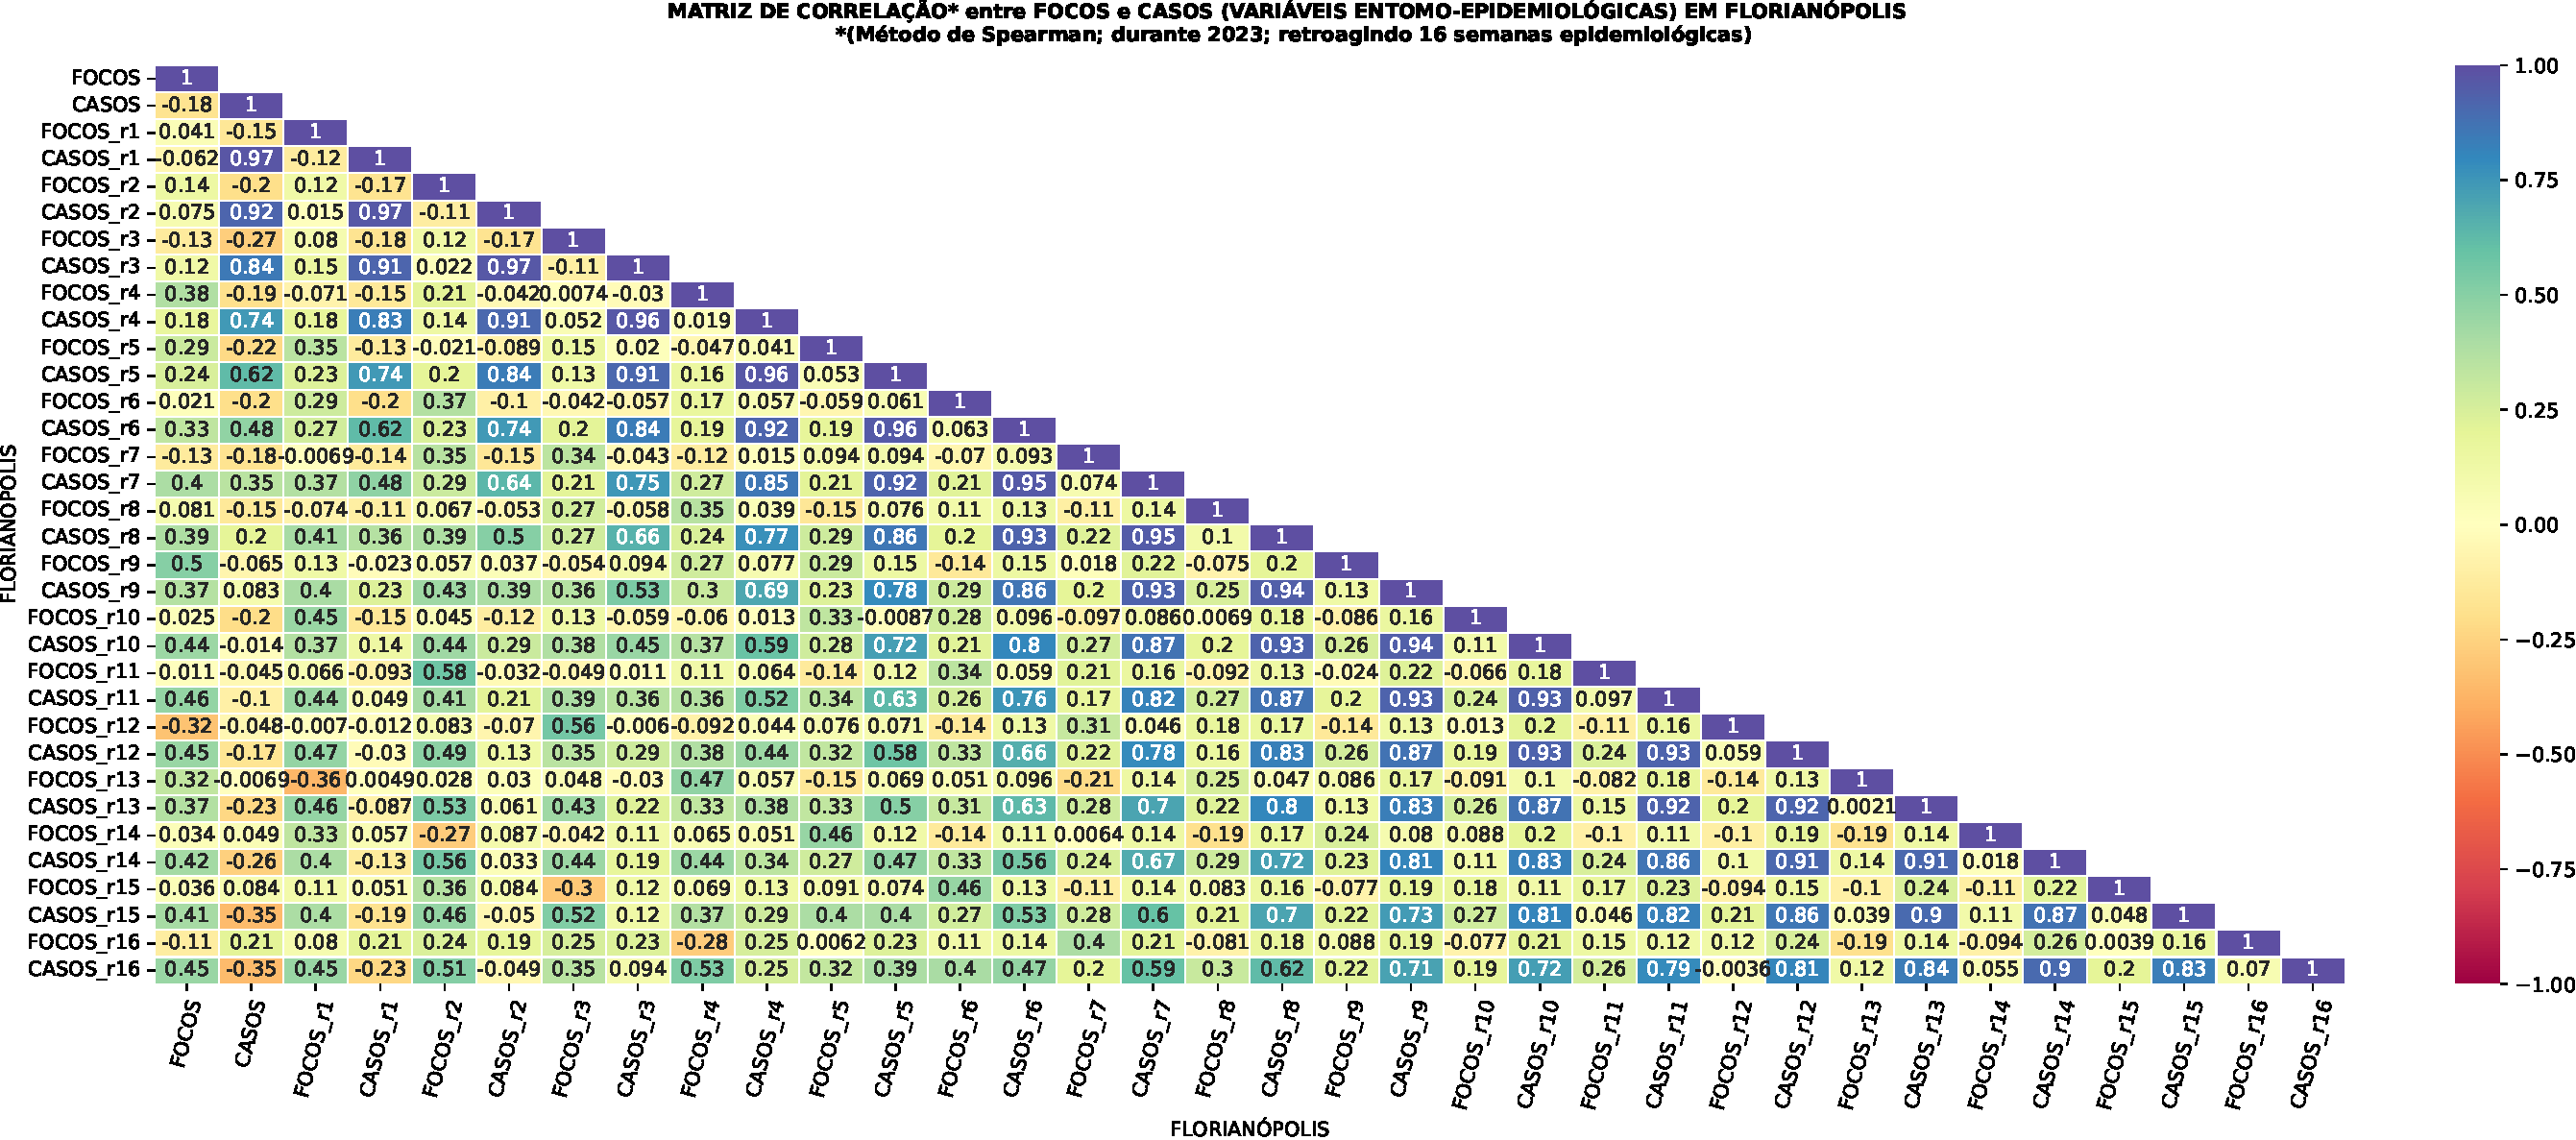
\includegraphics[width=0.47\textwidth]{figuras/matriz_correlacao_spearman_fococaso_FLORIANOPOLIS_r16s_2023.pdf}
        }
    \subfloat[Itajaí \label{fig: corr_DEE_ITA}]{
        \centering
        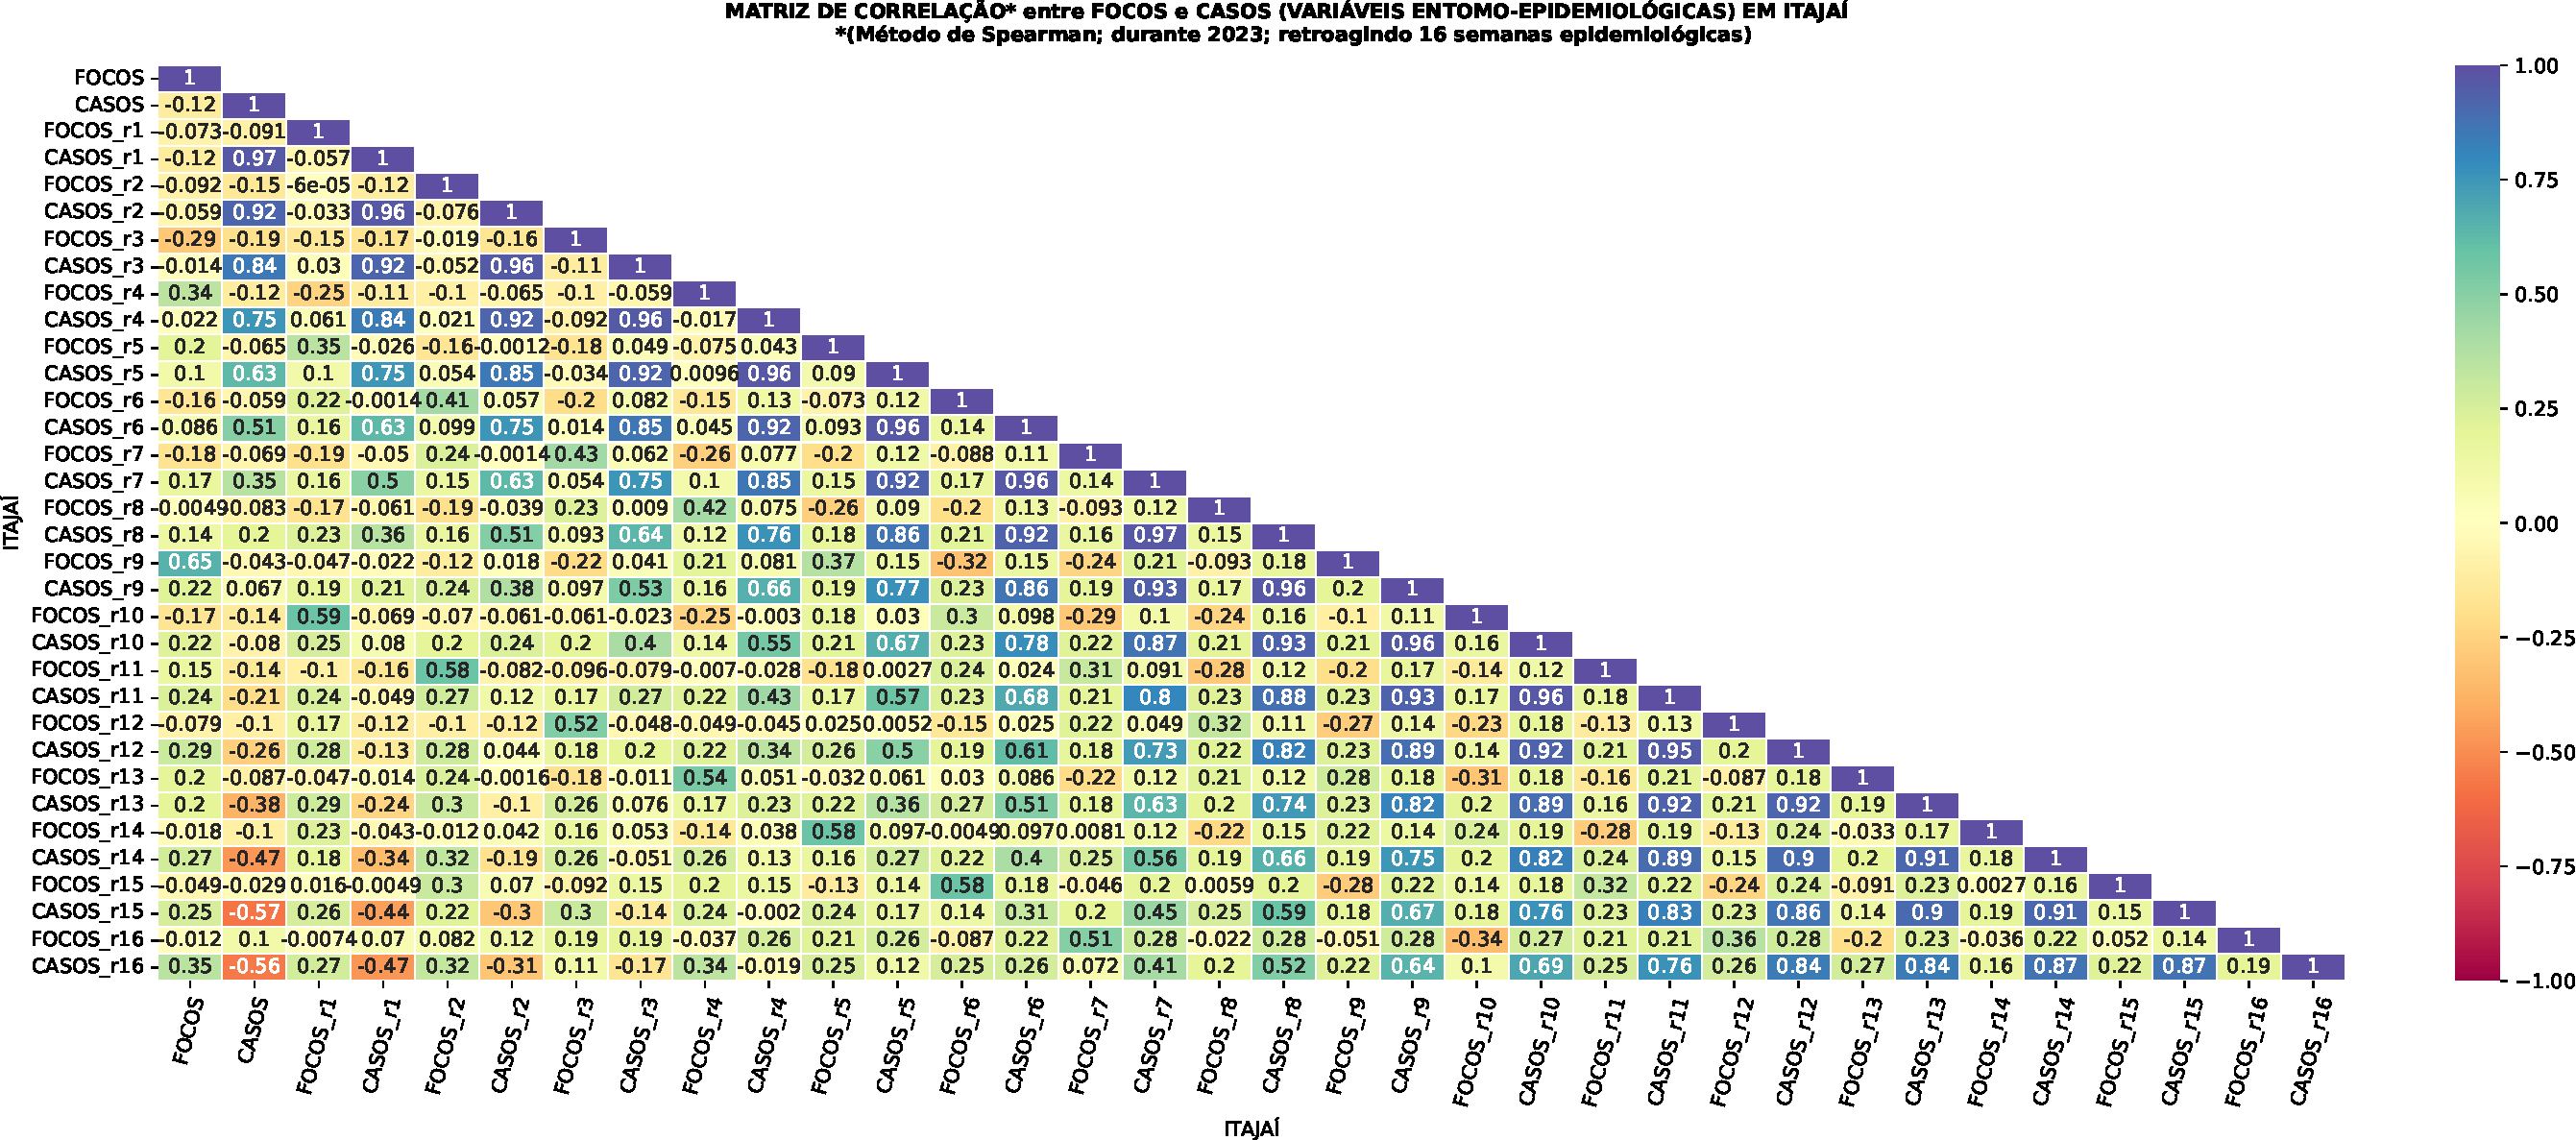
\includegraphics[width=0.47\textwidth]{figuras/matriz_correlacao_spearman_fococaso_ITAJAI_r16s_2023.pdf}
        }\hfill
    \subfloat[Joinville \label{fig: corr_DEE_JOI}]{
        \centering
        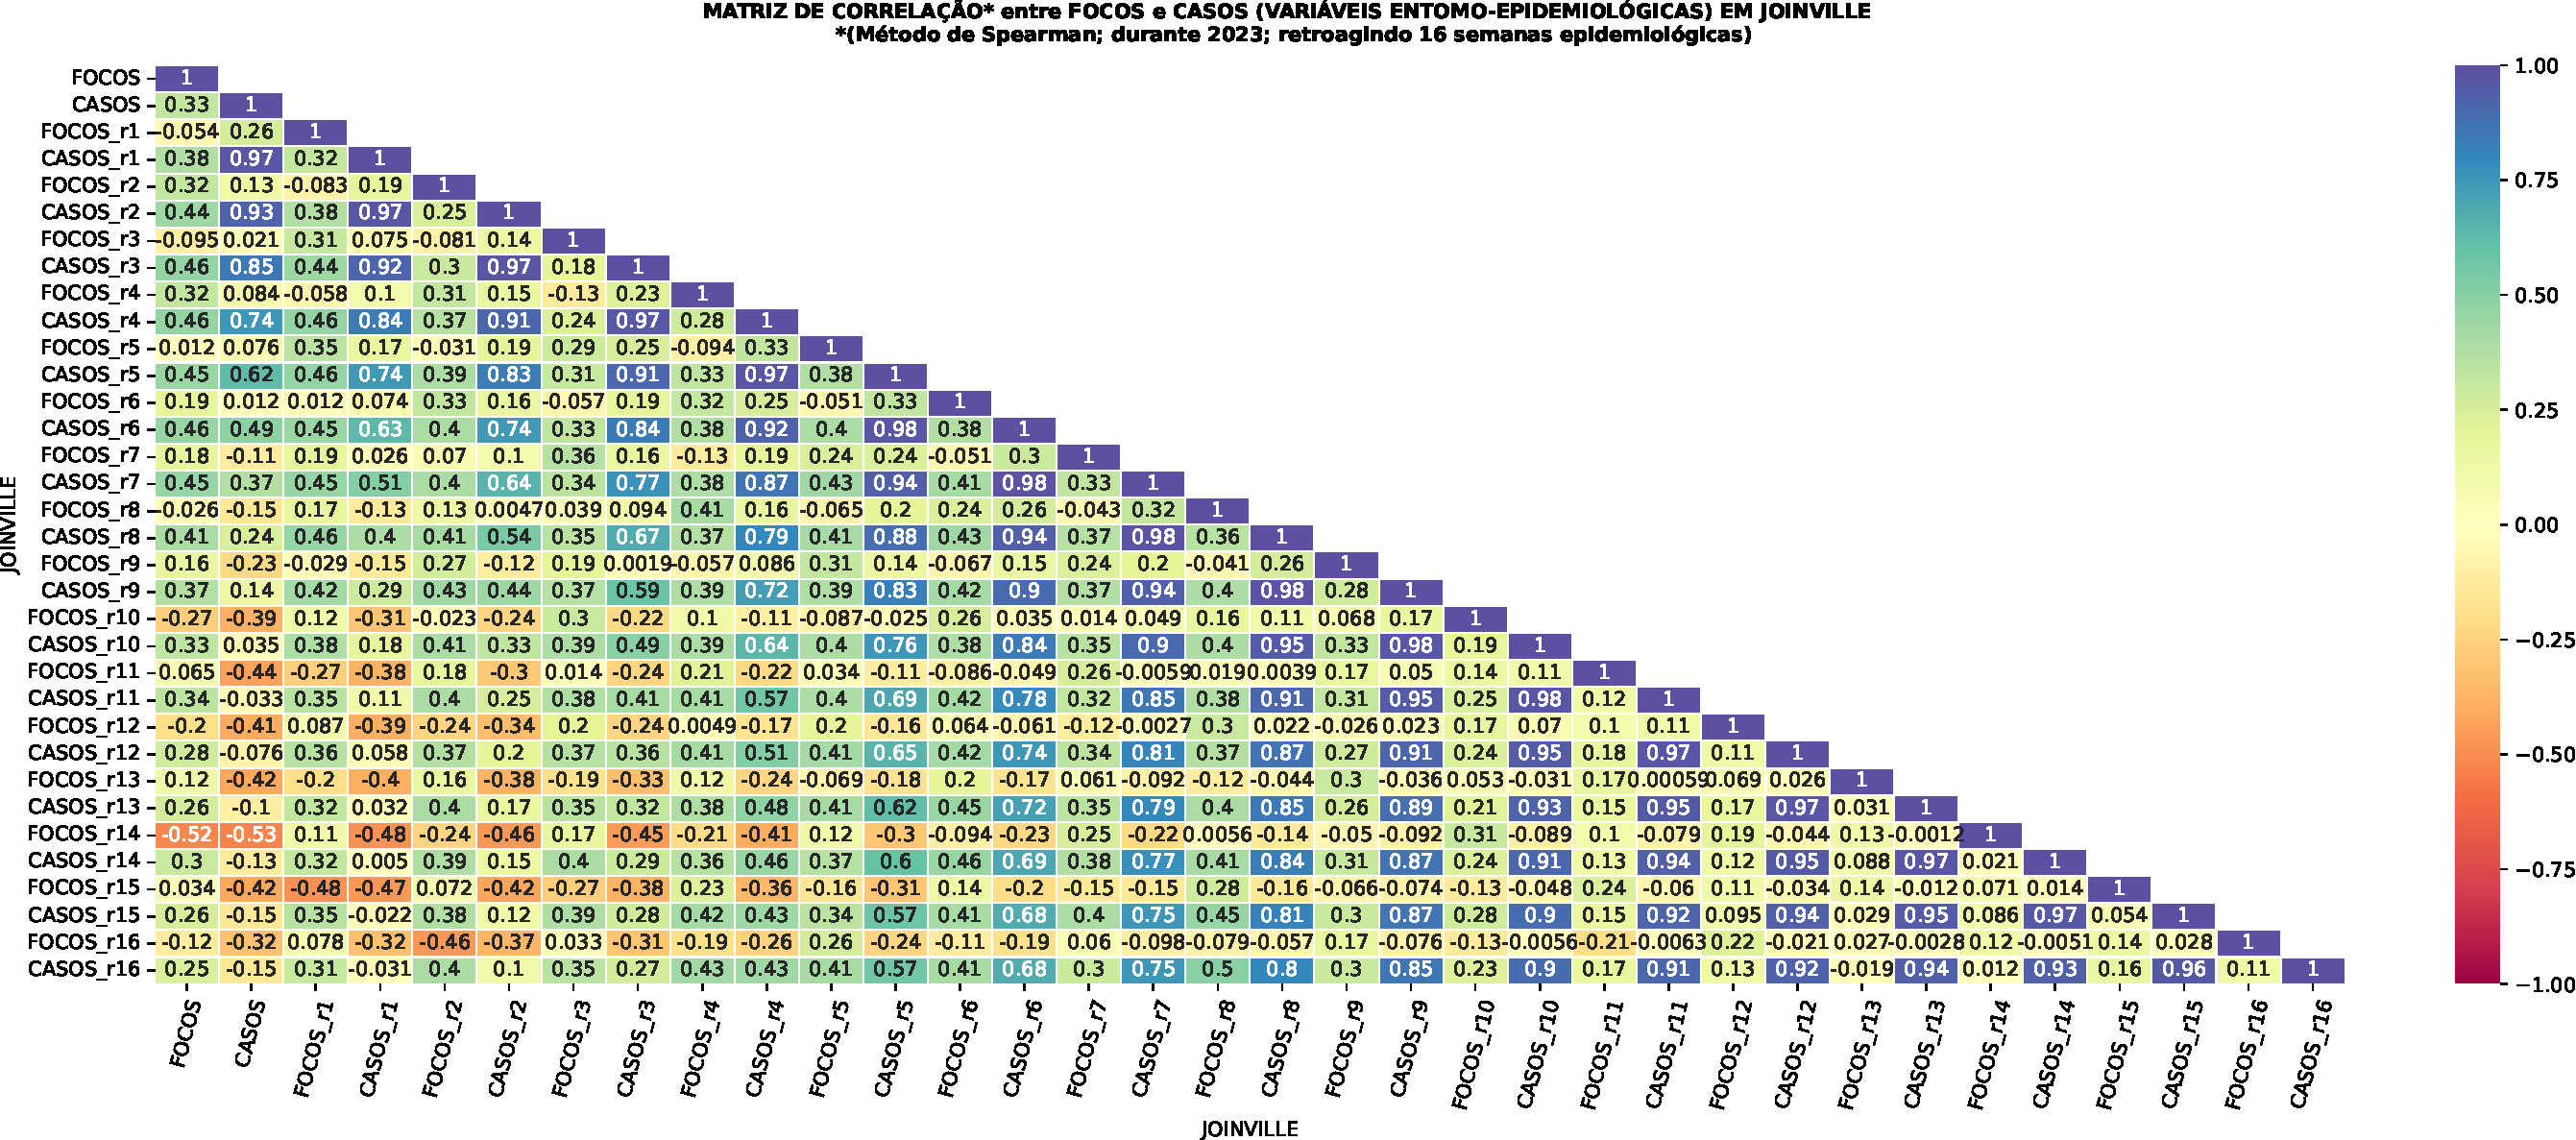
\includegraphics[width=0.47\textwidth]{figuras/matriz_correlacao_spearman_fococaso_JOINVILLE_r16s_2023.pdf}
        }
    \subfloat[Chapecó \label{fig: corr_DEE_CHA}]{
        \centering
        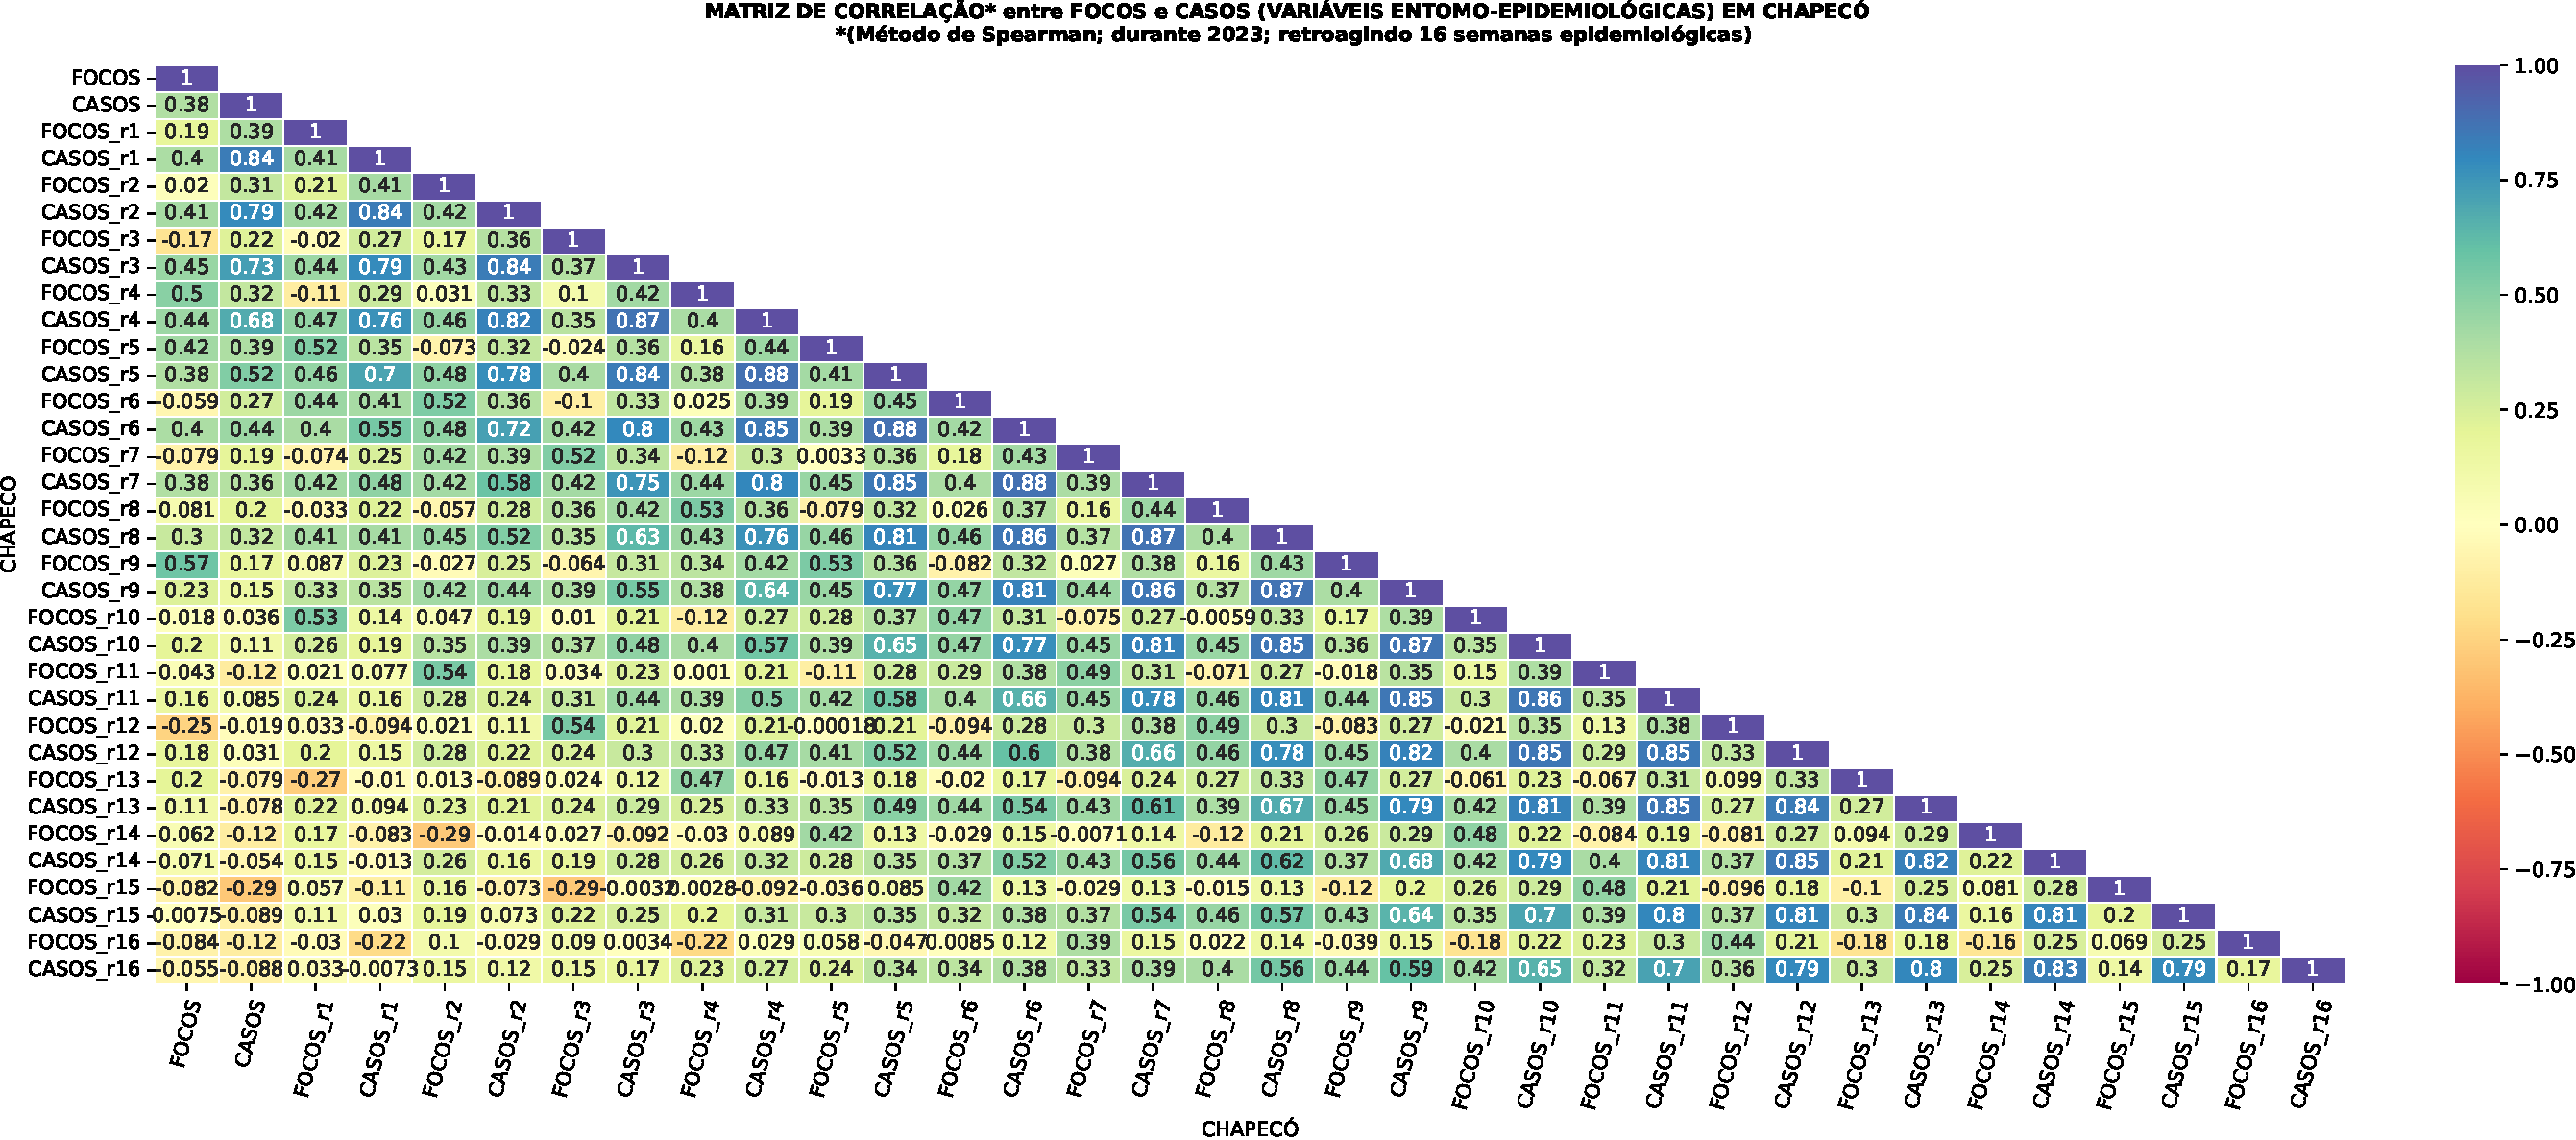
\includegraphics[width=0.47\textwidth]{figuras/matriz_correlacao_spearman_fococaso_CHAPECO_r16s_2023.pdf}
        }\hfill
    \end{center}
    \small{Fonte: Elaboração própria (2024).}
\end{figure}

Há flutuação entre os anos, porém ao correlacionar a série temporal integralmente (figura \ref{fig: matriz_corr_DEEtotal}), os municípios de Florianópolis (figura \ref{fig: corr_DEE_FLOtotal}) e Joinville (figura \ref{fig: corr_DEE_JOItotal}) apresentaram valores médios e altos de correlação em quase a totalidade da análise. Os municípios de Itajaí figura \ref{fig: corr_DEE_ITAtotal}) e Chapecó figura \ref{fig: corr_DEE_CHAtotal}) apresentaram valores baixos e médios, sendo apenas altos quando correlacionados com a própria variável pretérita.  \textcolor{red}{Por quê? Pode ser indicativo que esses municípios, Florianópolis e Joinville, apresentem relação de casos de dengue autóctones maior; enquanto outros municípios, como Chapecó e Itajaí, tenham importação de casos de dengue dentro da série temporal?}



\begin{figure}[htbp]
    \begin{center}
    \caption{Matriz de correlações entre focos de \latim{Aedes} sp. e casos de dengue de alguns municípios catarinenses durante a série histórica, método de Spearman.}
    \label{fig: matriz_corr_DEEtotal}
    \subfloat[Florianópolis \label{fig: corr_DEE_FLOtotal}]{
        \centering
        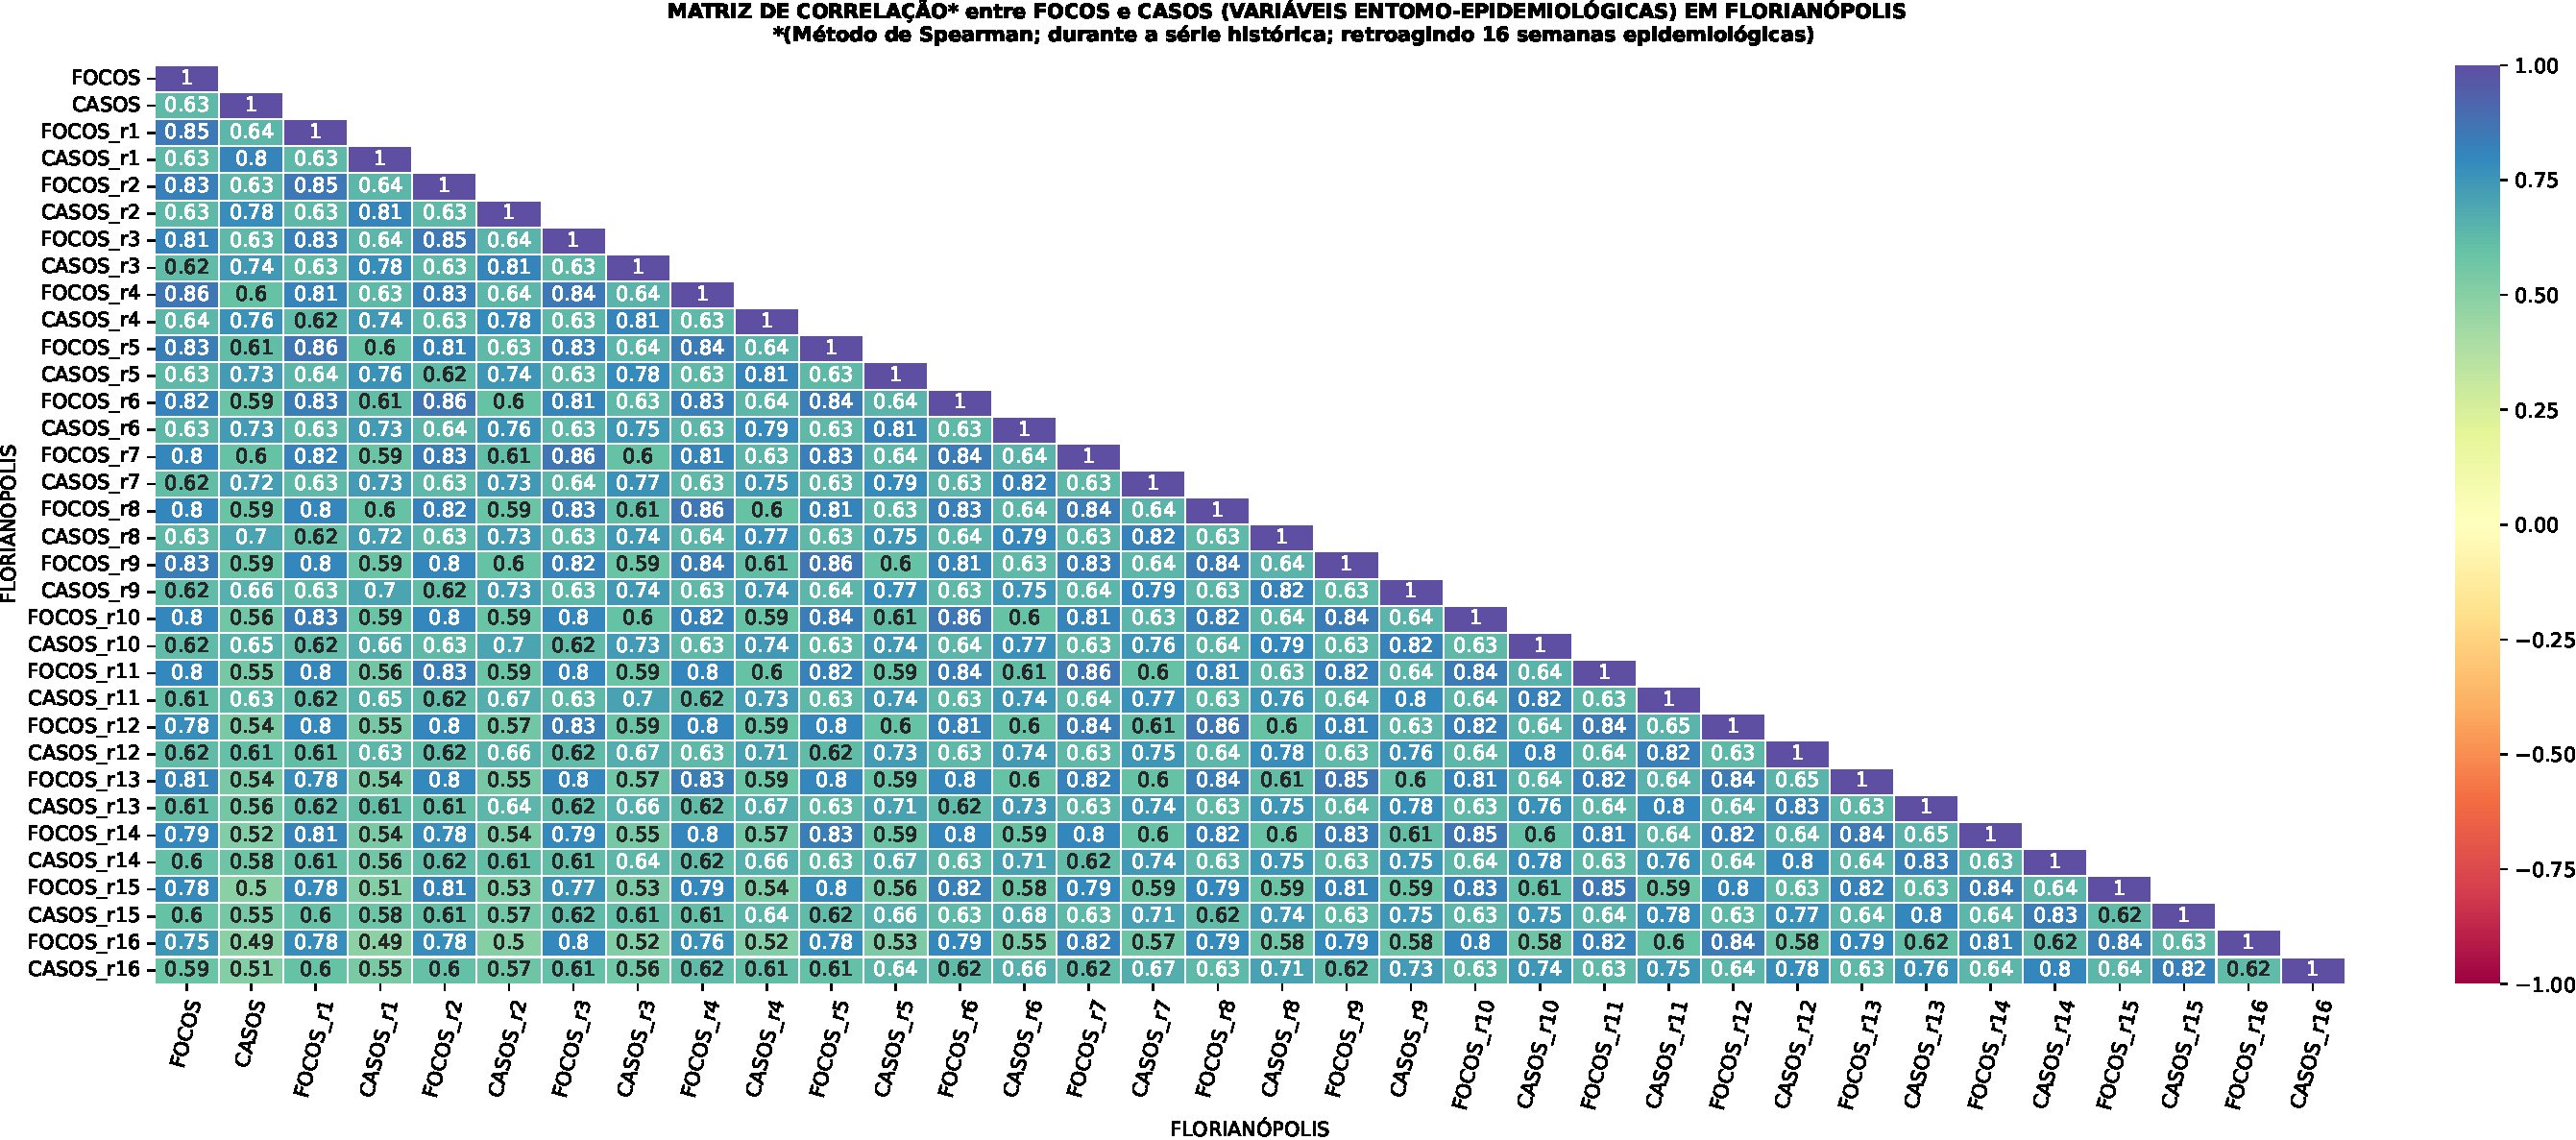
\includegraphics[width=0.47\textwidth]{figuras/matriz_correlacao_spearman_fococaso_FLORIANOPOLIS_r16s_total.pdf}
        }
    \subfloat[Itajaí \label{fig: corr_DEE_ITAtotal}]{
        \centering
        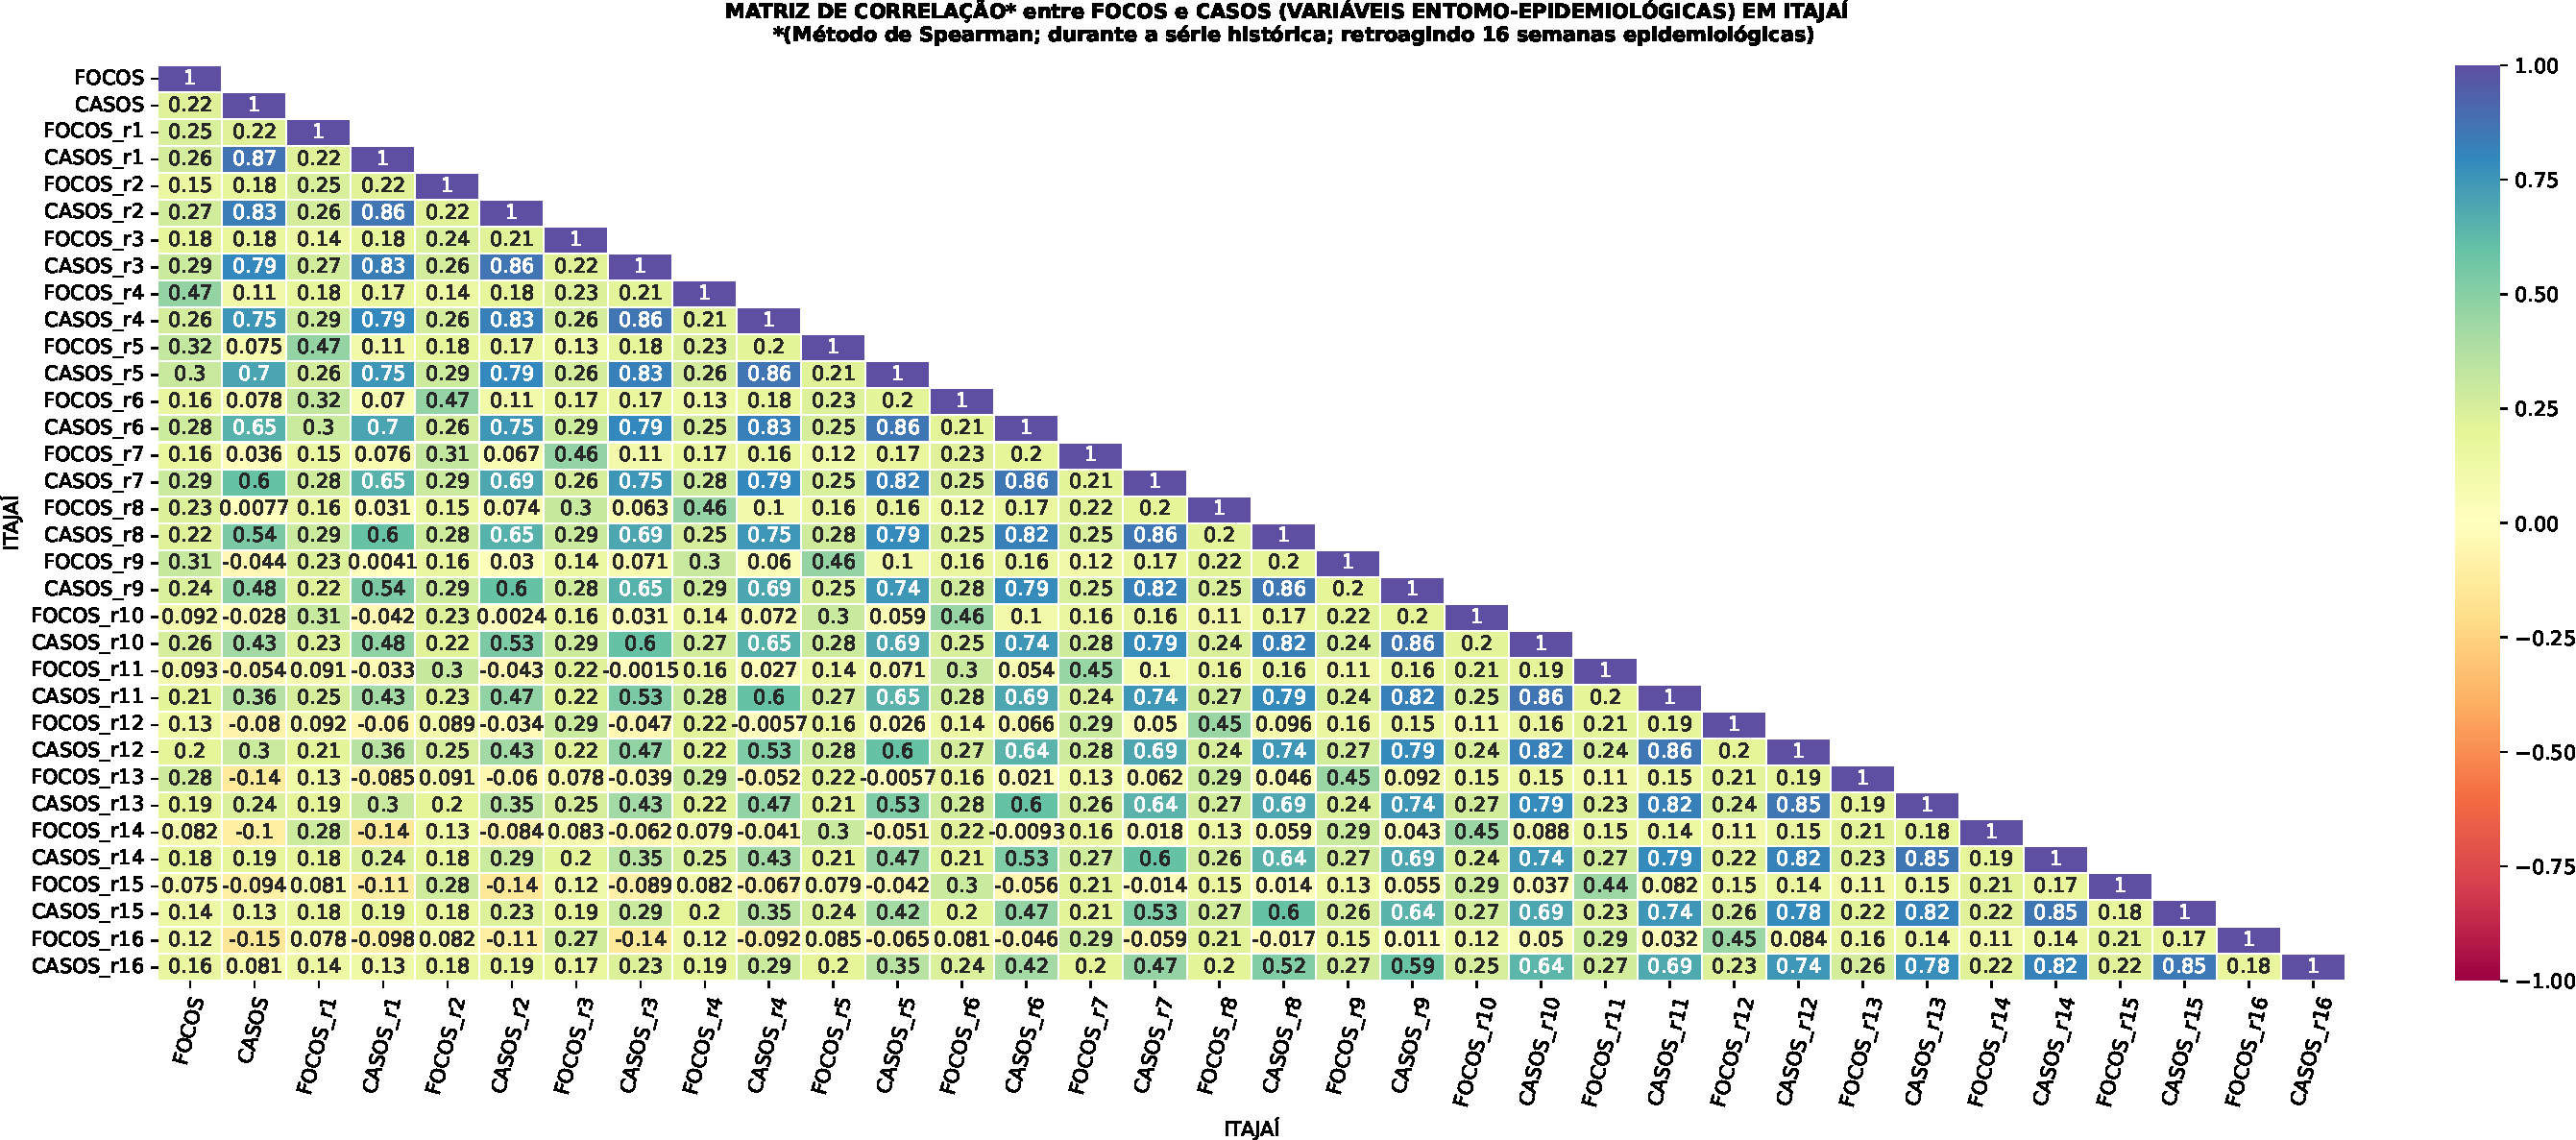
\includegraphics[width=0.47\textwidth]{figuras/matriz_correlacao_spearman_fococaso_ITAJAI_r16s_total.pdf}
        }\hfill
    \subfloat[Joinville \label{fig: corr_DEE_JOItotal}]{
        \centering
        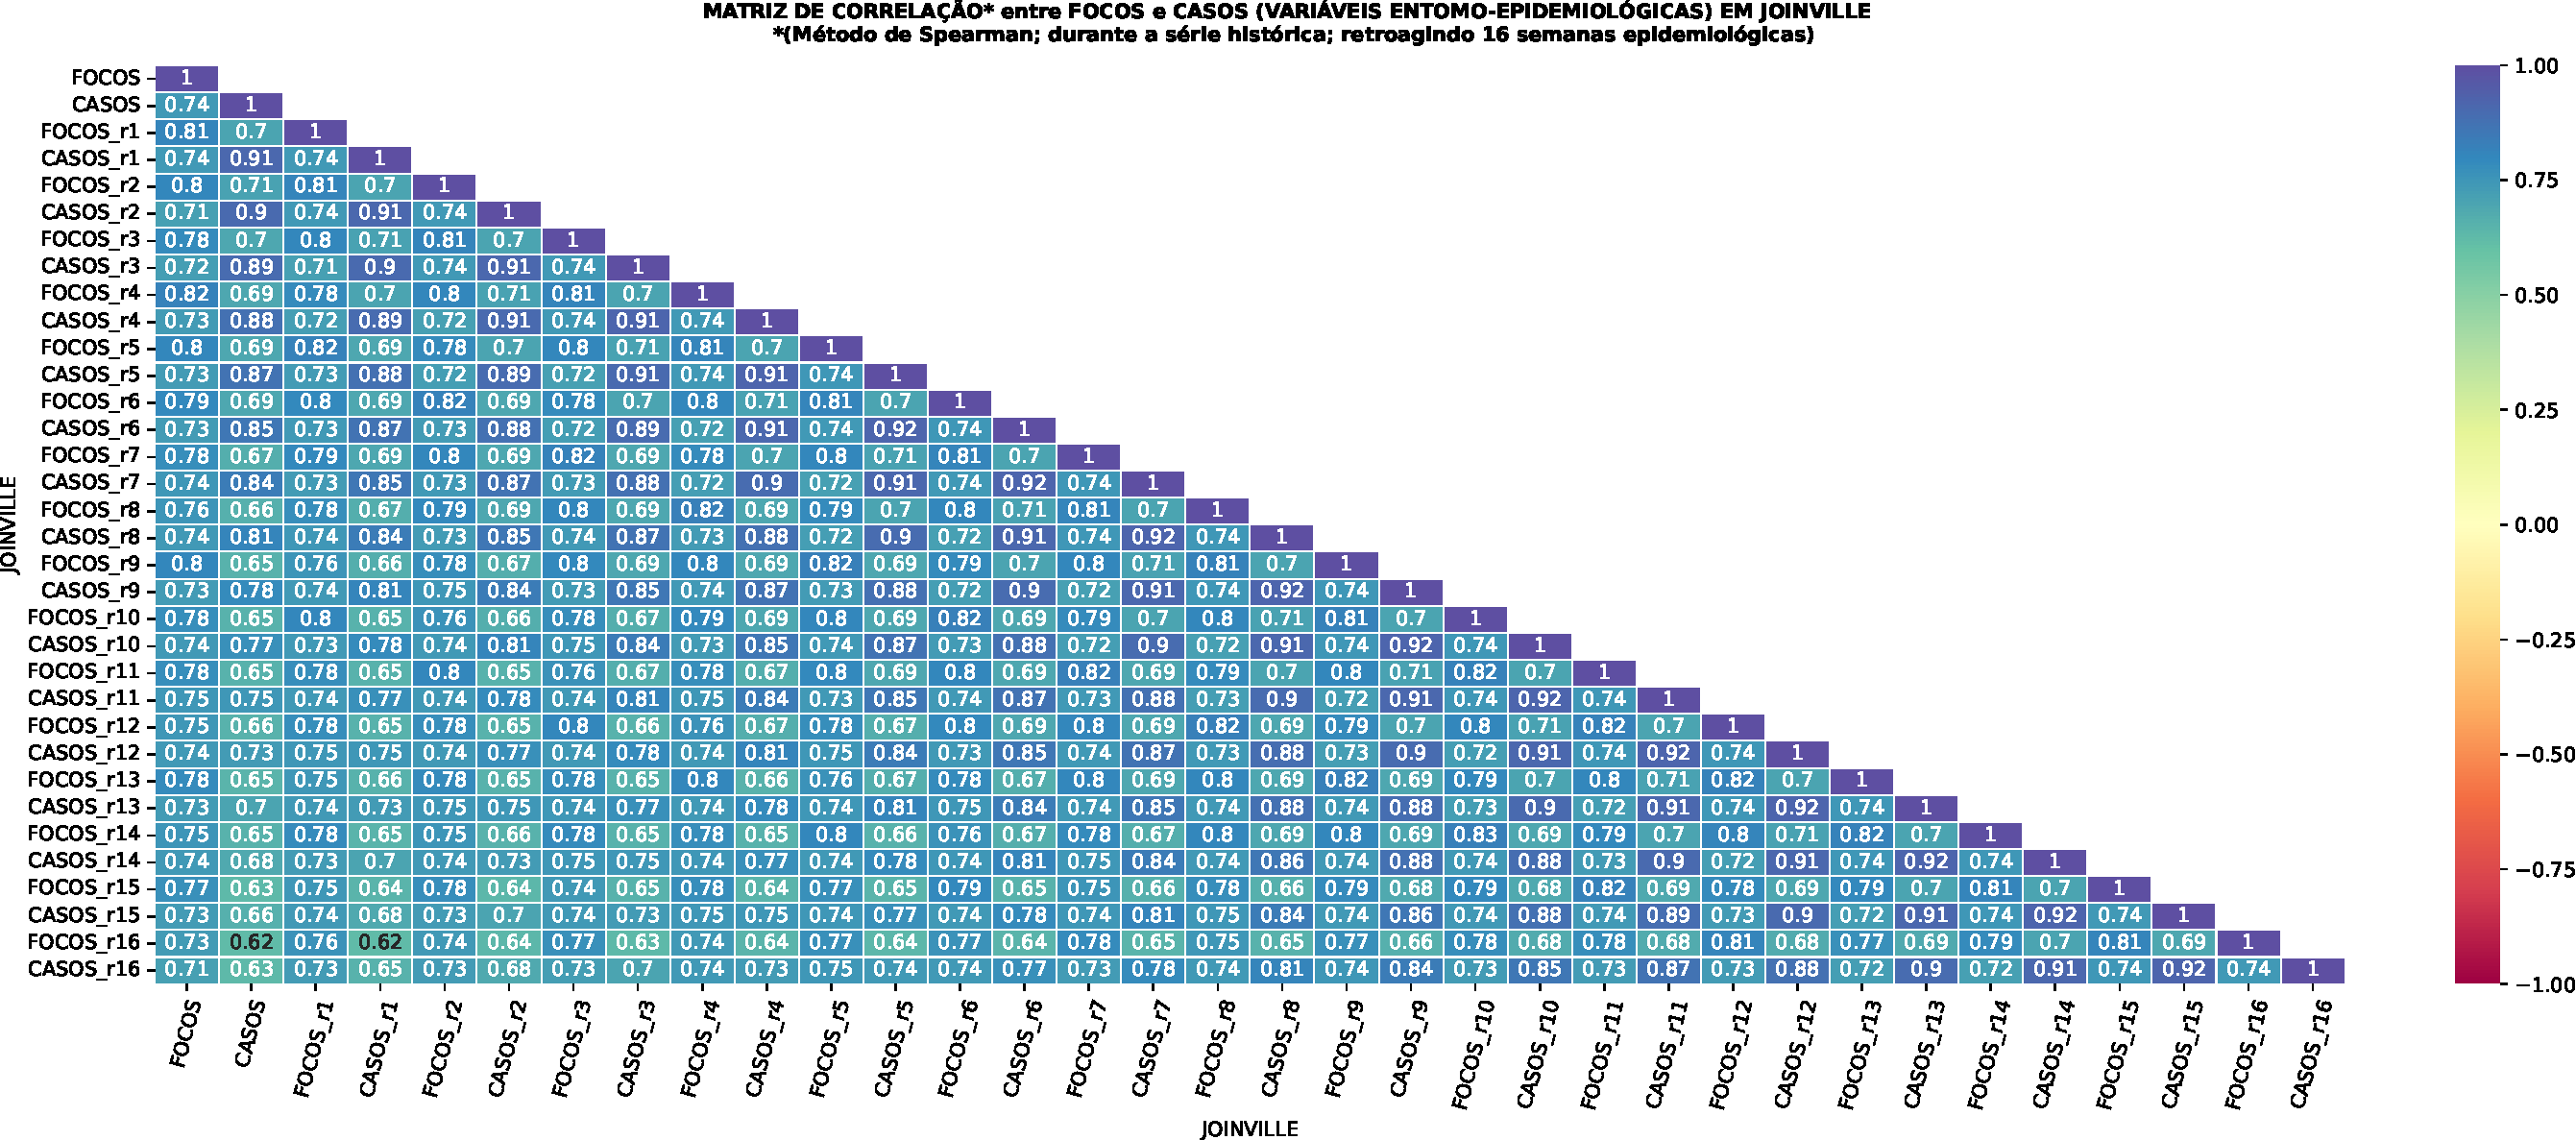
\includegraphics[width=0.47\textwidth]{figuras/matriz_correlacao_spearman_fococaso_JOINVILLE_r16s_total.pdf}
        }
    \subfloat[Chapecó \label{fig: corr_DEE_CHAtotal}]{
        \centering
        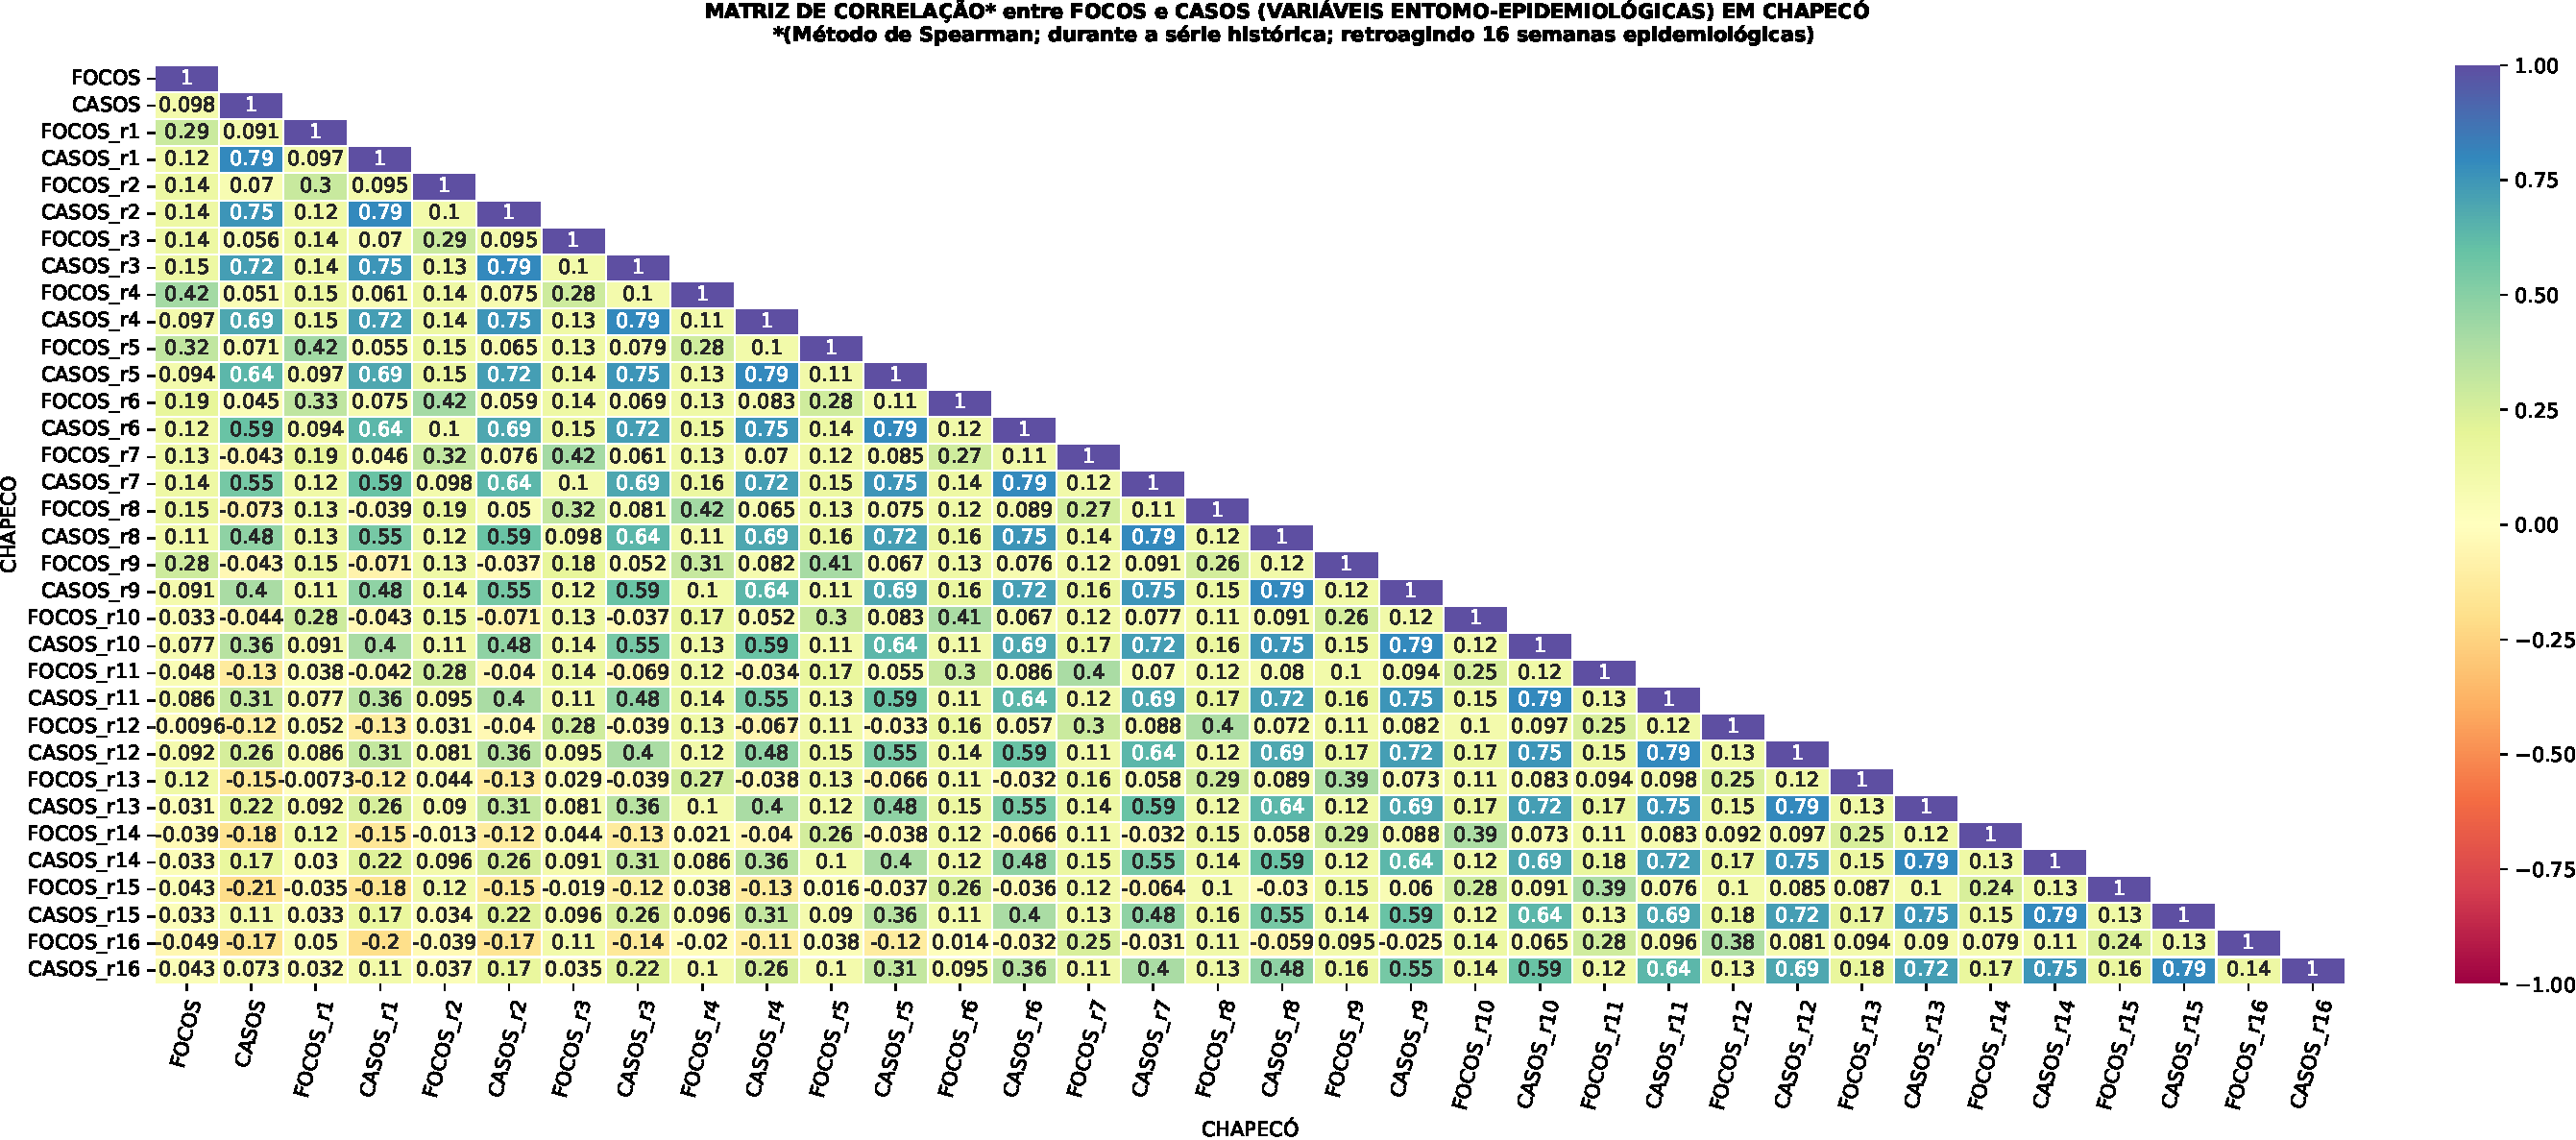
\includegraphics[width=0.47\textwidth]{figuras/matriz_correlacao_spearman_fococaso_CHAPECO_r16s_total.pdf}
        }\hfill
    \end{center}
    \small{Fonte: Elaboração própria (2024).}
\end{figure}

% entre esses elementos citados anteriormente e os \acrshort{DEC} (precipitação e temperaturas mínima, média e máxima)
\indent A correlação entre os \acrshort{DEE} (focos de \latim{Aedes} sp. e casos de dengue) e os \acrshort{DEC} (precipitação e temperaturas mínima, média e máxima) também foram realizadas pelo método de Spearman durante cada ano citado anteriormente (de 2020 a 2023) e a série histórica. Apenas duas variáveis climatológicas, temperatura média e precipitação, foram retrocedidas 16 semanas epidemiologicas. A temperatura média foi a escolhida para retroação pois, nas quatro (4) cidades, as correlaçãos entre ela e as temperaturas mínima e máxima se apresentaram altas, conforme apresentado nasanálises realizadas em 2023 (figura \ref{fig: matriz_corr_CLI}). A capital catarinense, Florianópolis (figura \ref{fig: corr_CLI_FLO}), apresentou correlação média positiva entre focos de \latim{Aedes} sp. e temperaturas mínima, média e máxima; quando retroativas, oscilam entre média e baixa, também evidenciado na precipitação. O município de Itajaí (figura \ref{fig: corr_CLI_ITA}) apresentou correlação média positiva entre focos de \latim{Aedes} sp. e a precipitação retrocedida duas (2) semanas epidemiológicas. O município de Chapecó (figura \ref{fig: corr_CLI_CHAtotal}) apresentou correlação média positiva entre focos de \latim{Aedes} sp. e casos de dengue, temperatura média e temperatura máxima, sem retroação; ao retroceder uma (1) semana epidemiológica, apresentou correlação baixa positiva entre focos de \latim{Aedes} sp. e precipitação. Todos os municípios apresentaram aumento na intensidade da correlação, atingindo correlação média negativa, ao passo que retrocede entre casos de dengue e temperatura média, oscilando de forma semelhante entre precipitação e casos de dengue. \textcolor{red}{Por quê?}

\begin{figure}[htbp]
    \begin{center}
    \caption{Matriz de correlações entre focos de \latim{Aedes} sp., casos de dengue e variáveis climatológicas de alguns municípios catarinenses durante 2023, método de Spearman.}
    \label{fig: matriz_corr_CLI}
    \subfloat[Florianópolis \label{fig: corr_CLI_FLO}]{
        \centering
        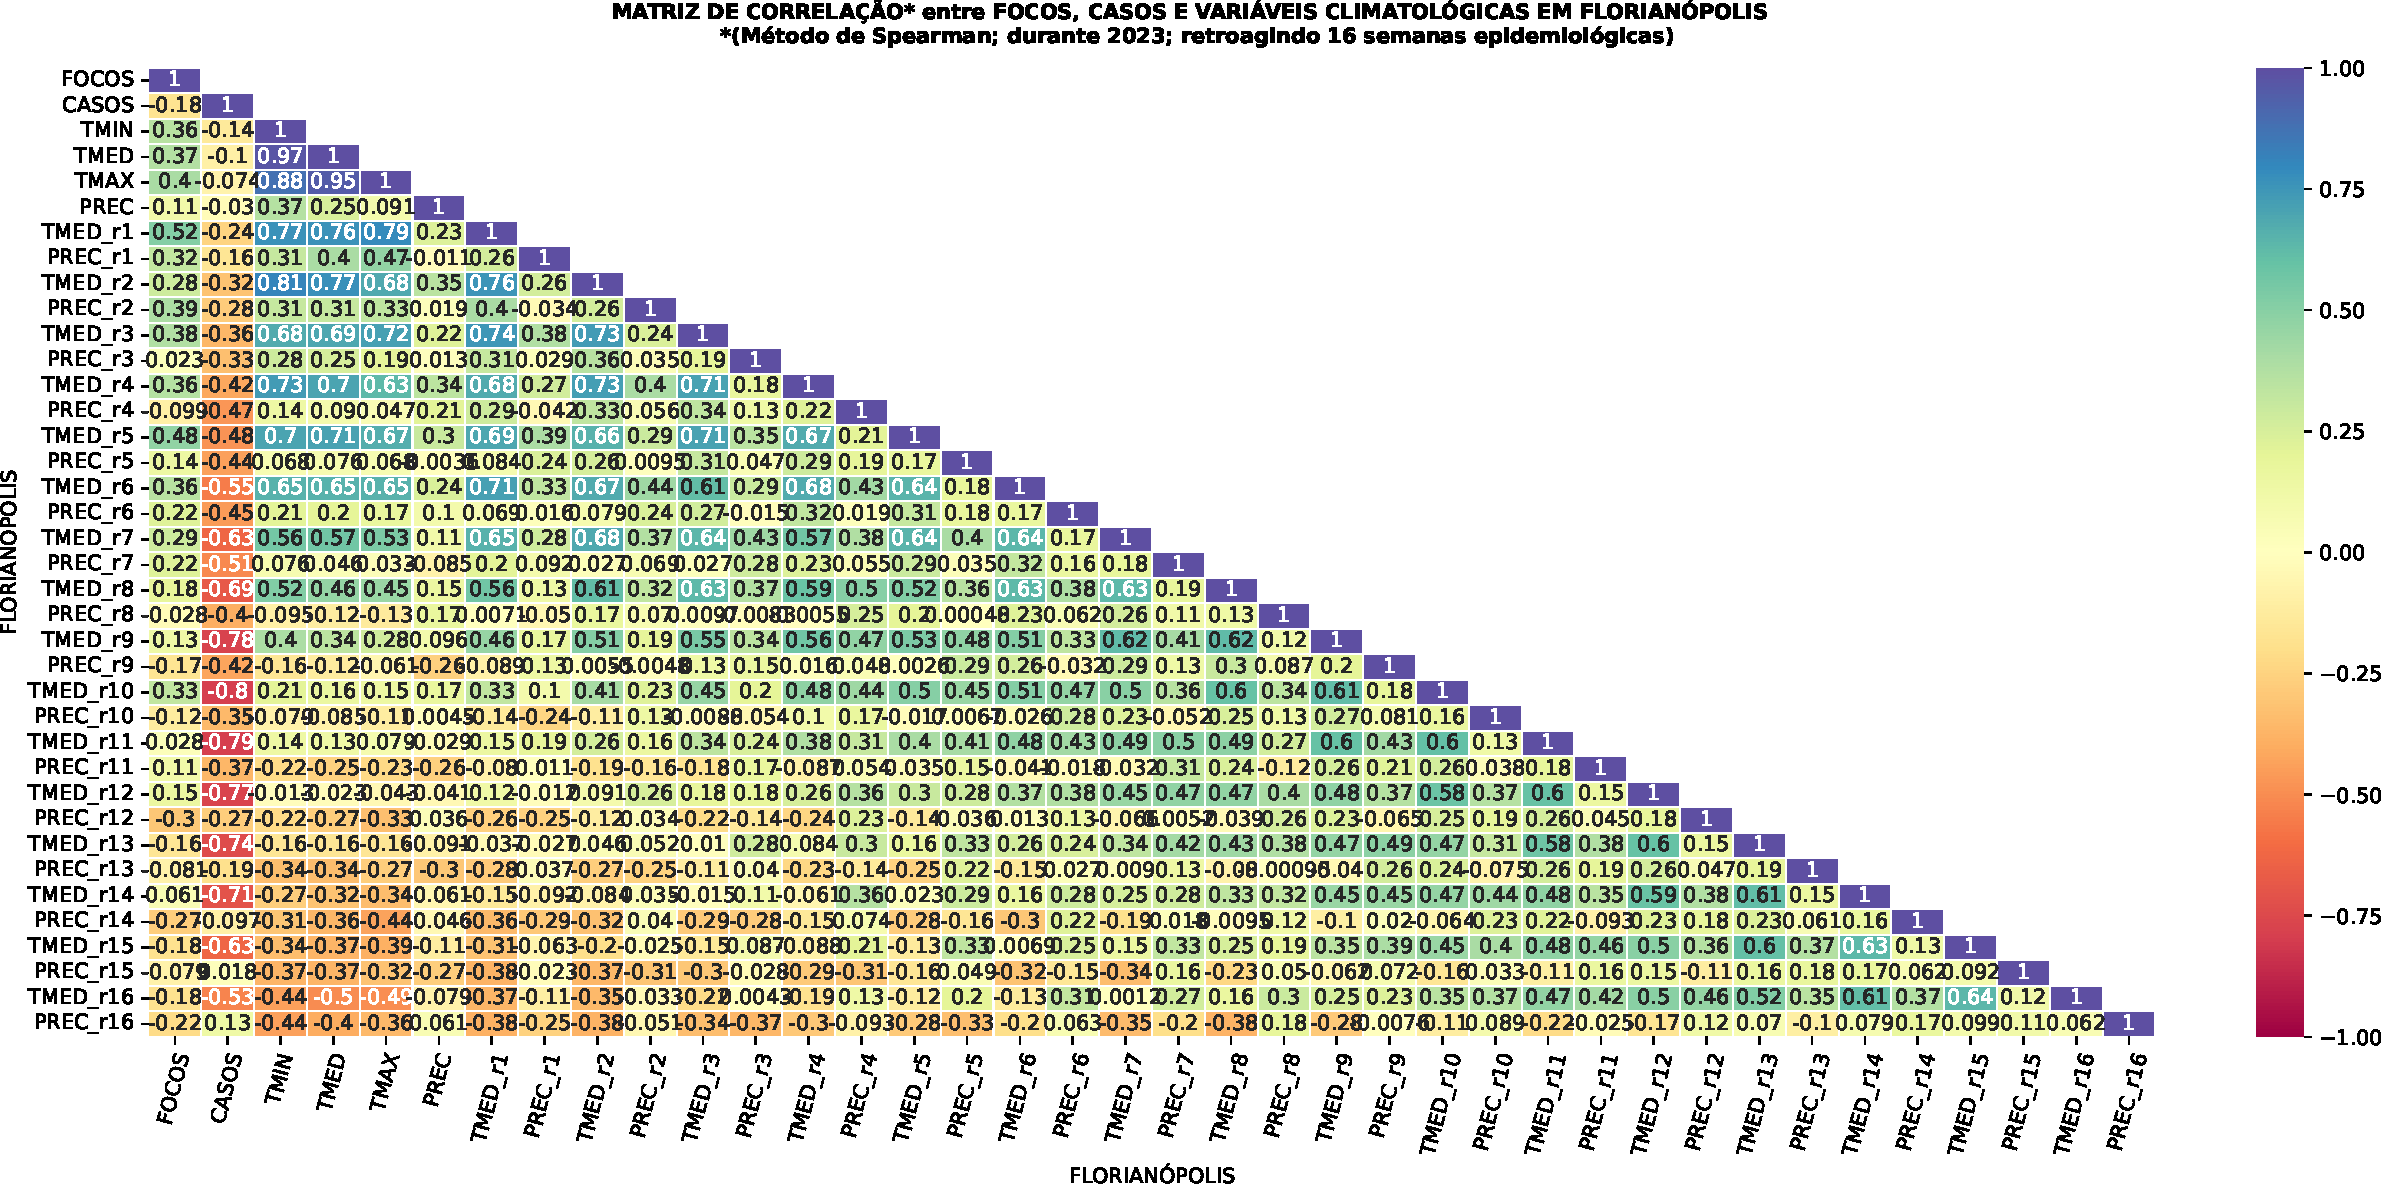
\includegraphics[width=0.47\textwidth]{figuras/matriz_correlacao_spearman_FLORIANOPOLIS_r16s_2023.pdf}
        }
    \subfloat[Itajaí \label{fig: corr_CLI_ITA}]{
        \centering
        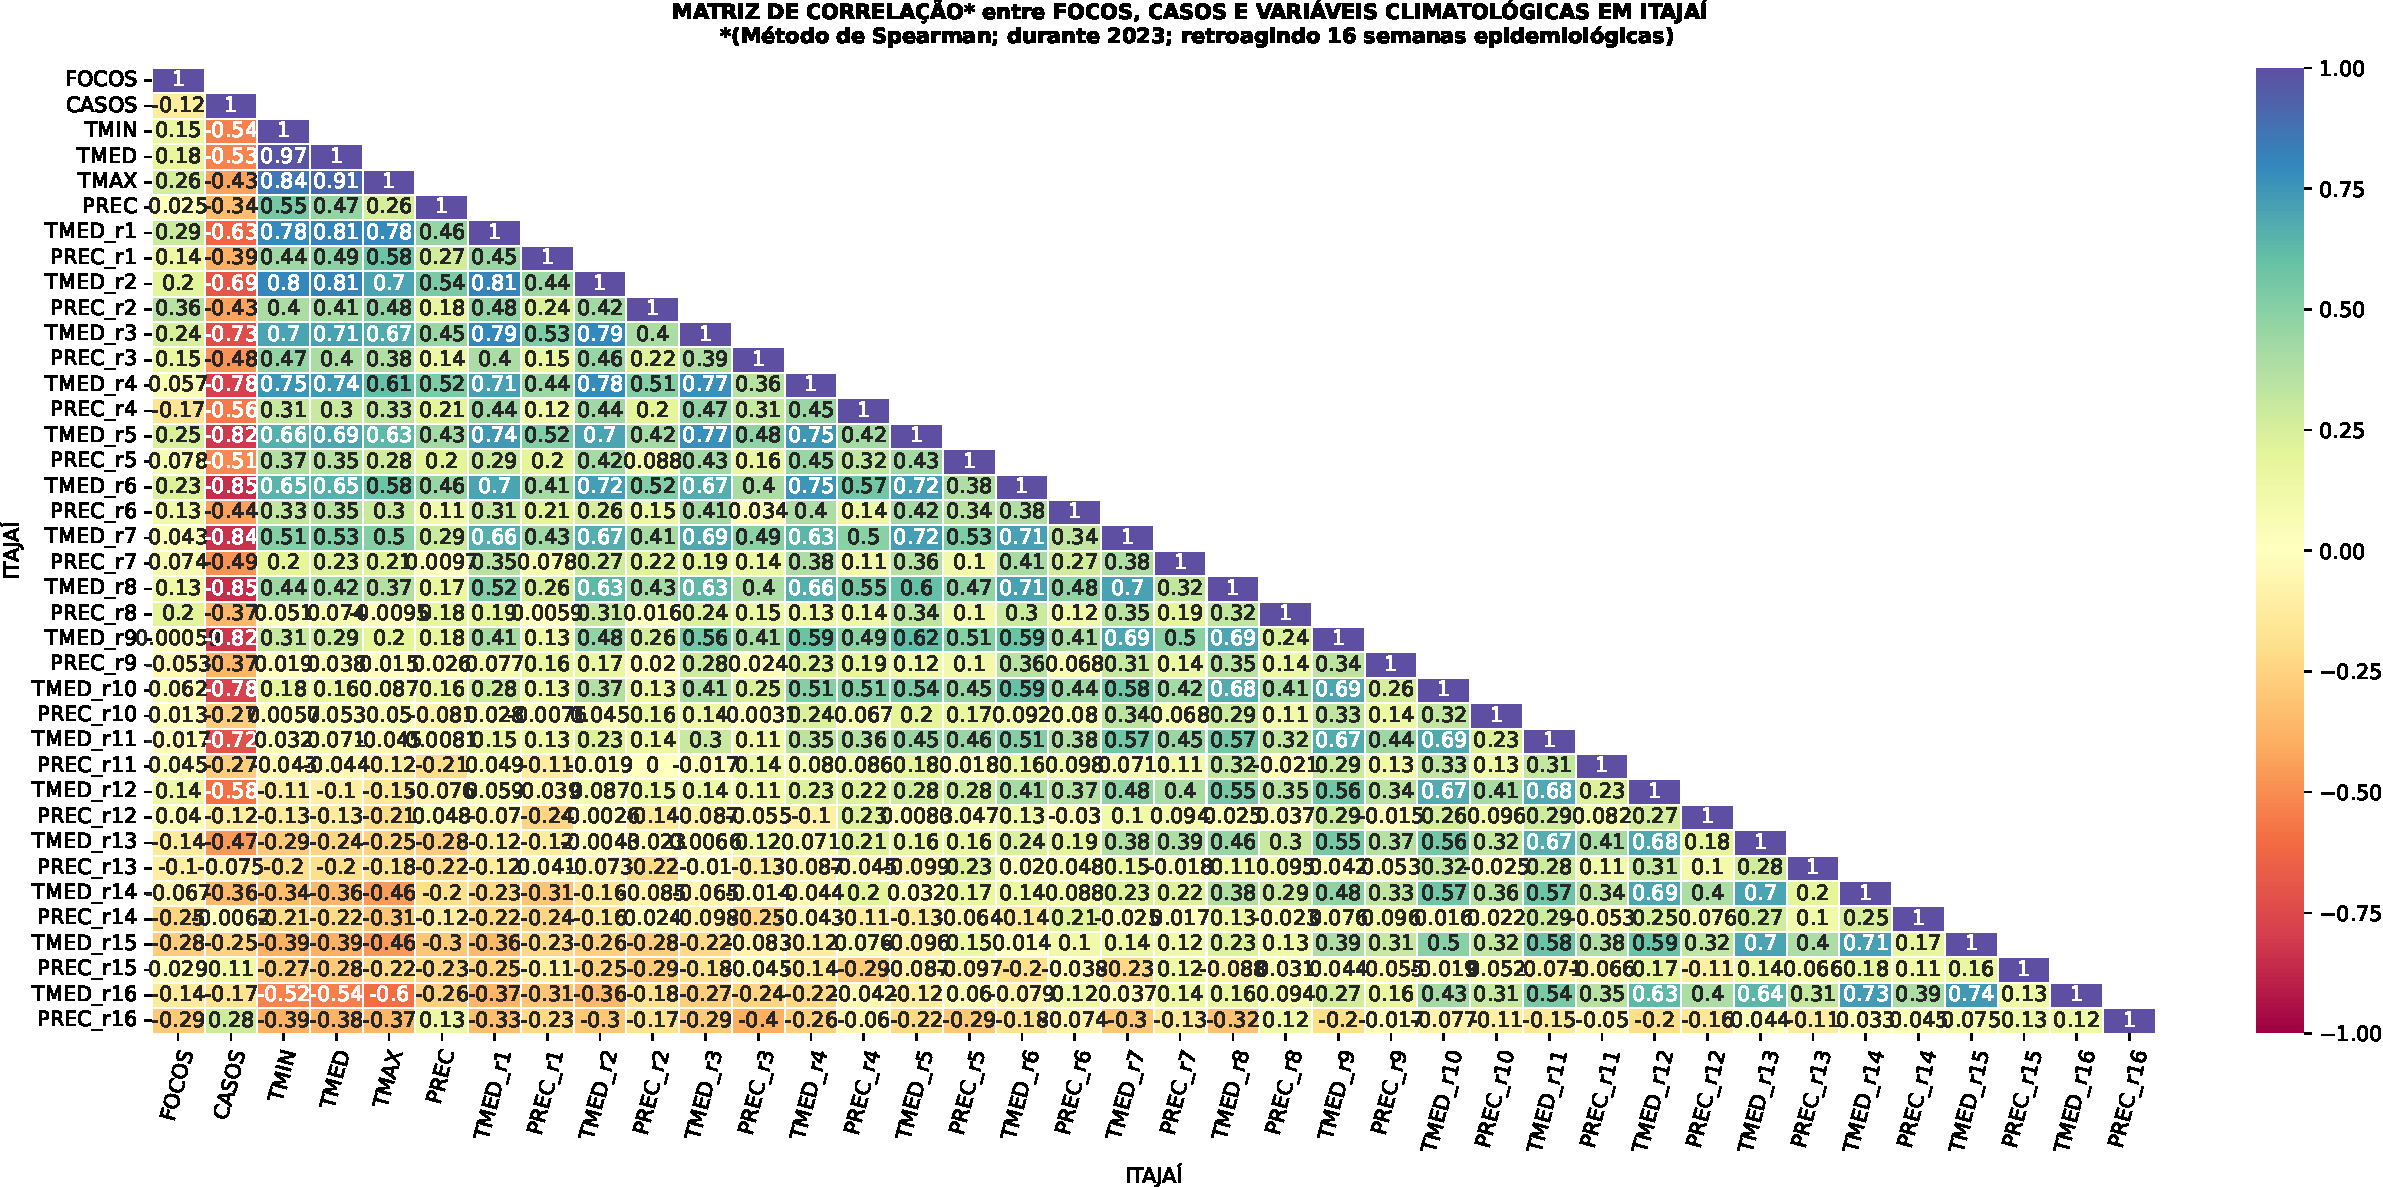
\includegraphics[width=0.47\textwidth]{figuras/matriz_correlacao_spearman_ITAJAI_r16s_2023.pdf}
        }\hfill
    \subfloat[Joinville \label{fig: corr_CLI_JOI}]{
        \centering
        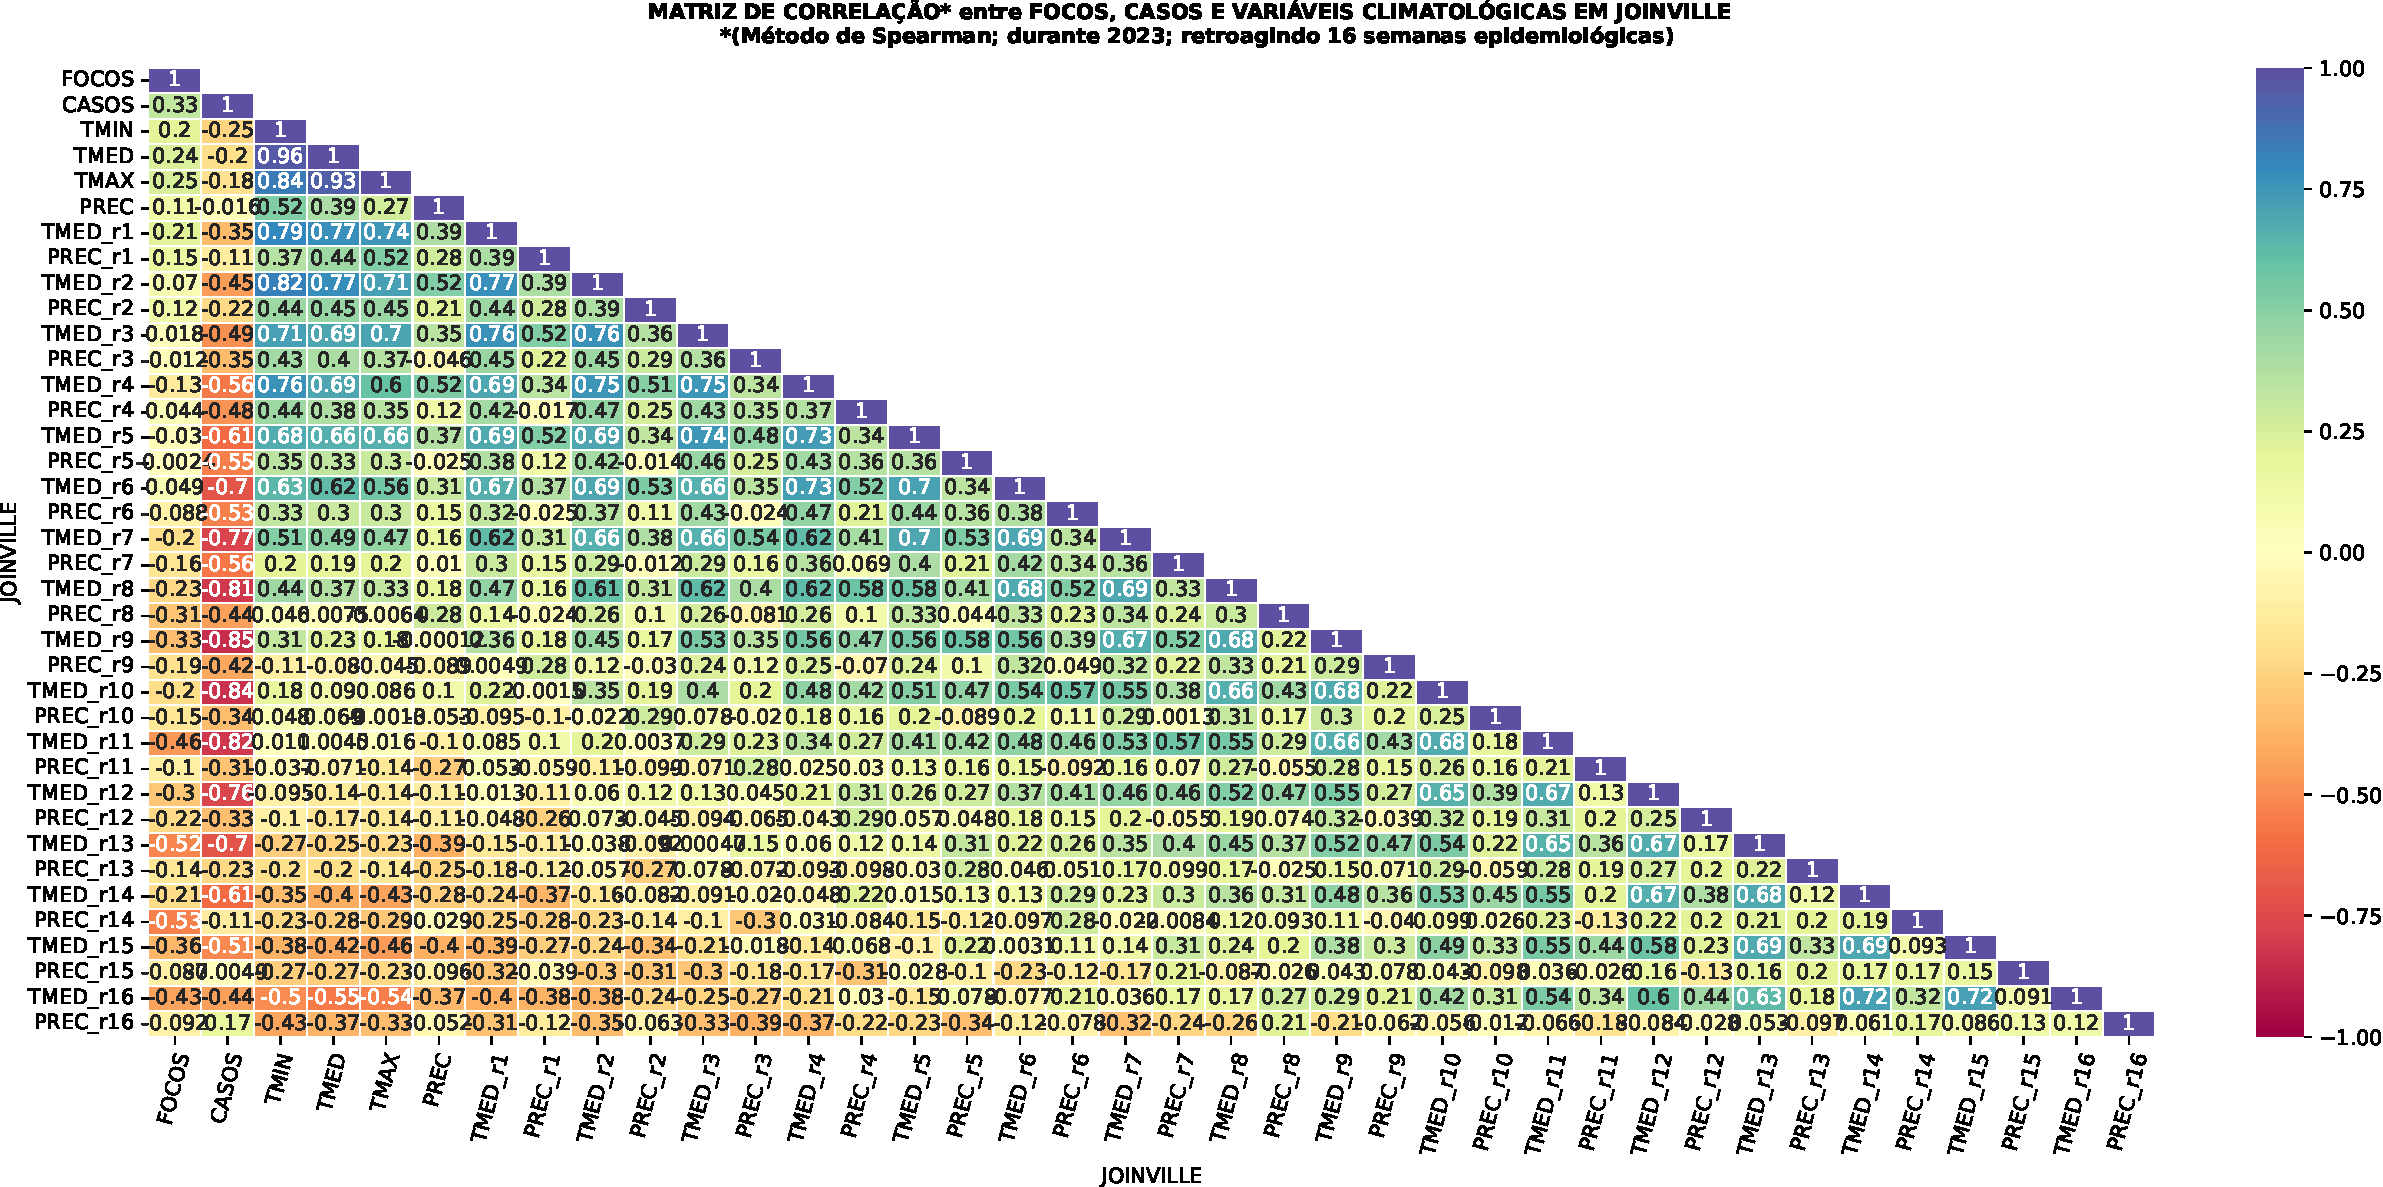
\includegraphics[width=0.47\textwidth]{figuras/matriz_correlacao_spearman_JOINVILLE_r16s_2023.pdf}
        }
    \subfloat[Chapecó \label{fig: corr_CLI_CHA}]{
        \centering
        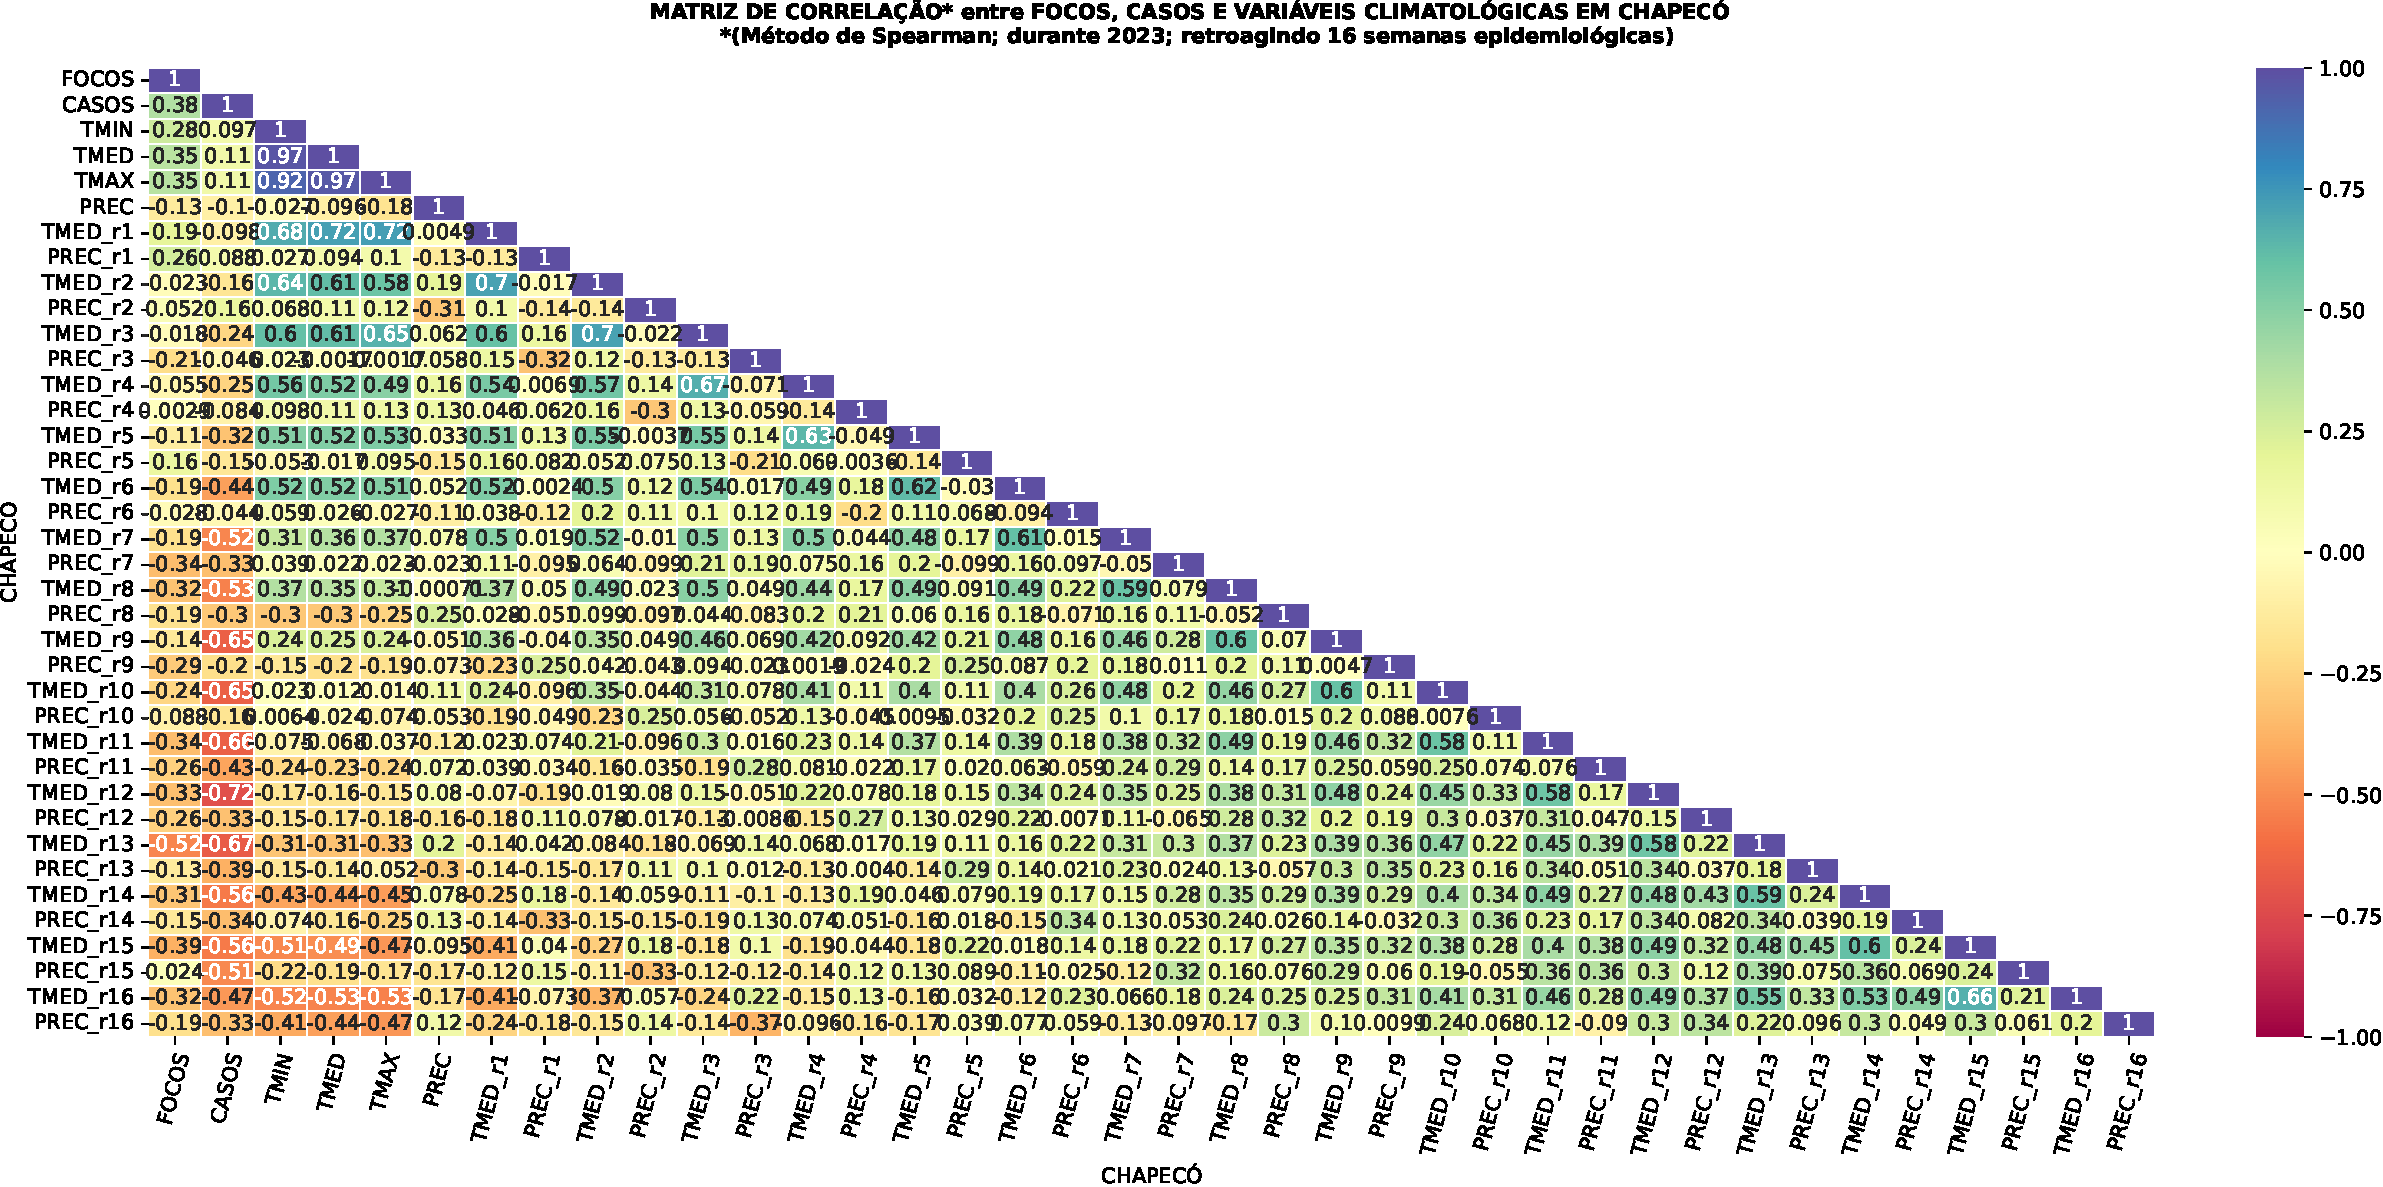
\includegraphics[width=0.47\textwidth]{figuras/matriz_correlacao_spearman_CHAPECO_r16s_2023.pdf}
        }\hfill
    \end{center}
    \small{Fonte: Elaboração própria (2024).}
\end{figure}

Também há flutuação entre os anos, porém ao correlacionar a série temporal integralmente (figura \ref{fig: matriz_corr_CLItotal}). Os municípios de Itajaí (figura \ref{fig: corr_CLI_ITAtotal}) e Chapecó (figura \ref{fig: corr_CLI_CHAtotal}) apresentaram aumento na intensidade da correlação, atingindo correlação média negativa, quando se retrocede a temperatura média com os casos de dengue. \textcolor{red}{Por quê?} O município de Joinville (figura \ref{fig: corr_CLI_JOItotal}) é o único que apresenta correlação média positiva entre a precipitação e as temperaturas, mesmo quando pouco retroagidas. Sugere-se a própria conformação de relevo do município, onde a temperatura aumenta a evaporação, aumentando a precipitação da umidade suspensa represada na Serra do Mar. Em todos os municípios, as variáveis climatológicas entre si, em especial as temperaturas, apresentaram valores médios e altos de correlação. Esse fato sugere certa estabilidade no sistema climatológico catarinense, pouco evidenciado na precipitação por conta do agrupamento semanal.

\begin{figure}[htbp]
    \begin{center}
    \caption{Matriz de correlações entre focos de \latim{Aedes} sp., casos de dengue e variáveis climatológicas de alguns municípios catarinenses durante a série histórica, método de Spearman.}
    \label{fig: matriz_corr_CLItotal}
    \subfloat[Florianópolis \label{fig: corr_CLI_FLOtotal}]{
        \centering
        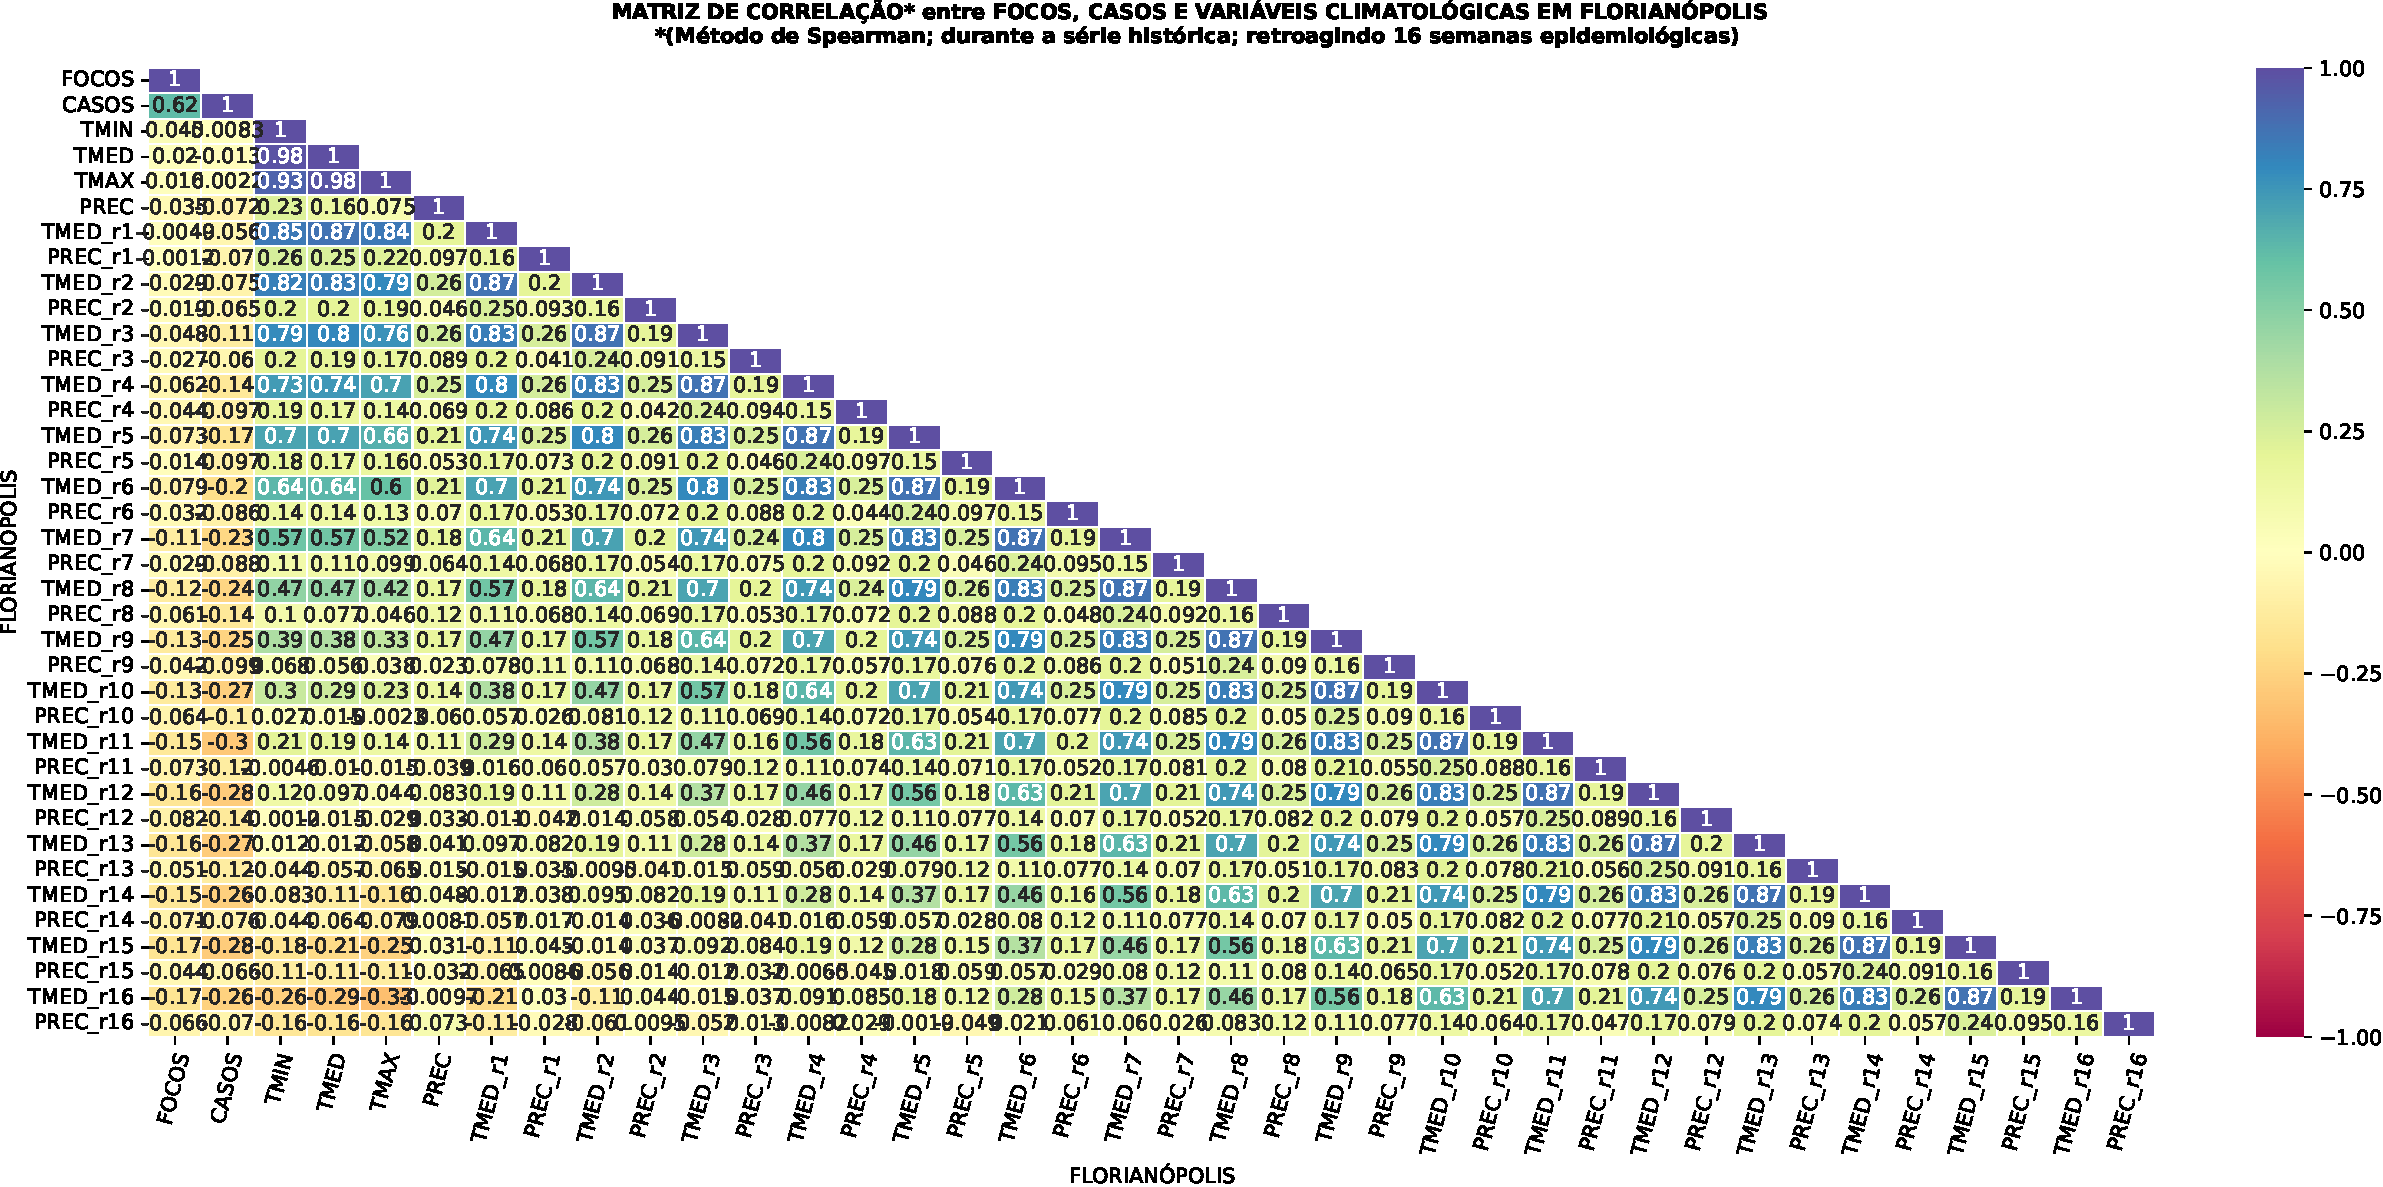
\includegraphics[width=0.47\textwidth]{figuras/matriz_correlacao_spearman_FLORIANOPOLIS_r16s_total.pdf}
        }
    \subfloat[Itajaí \label{fig: corr_CLI_ITAtotal}]{
        \centering
        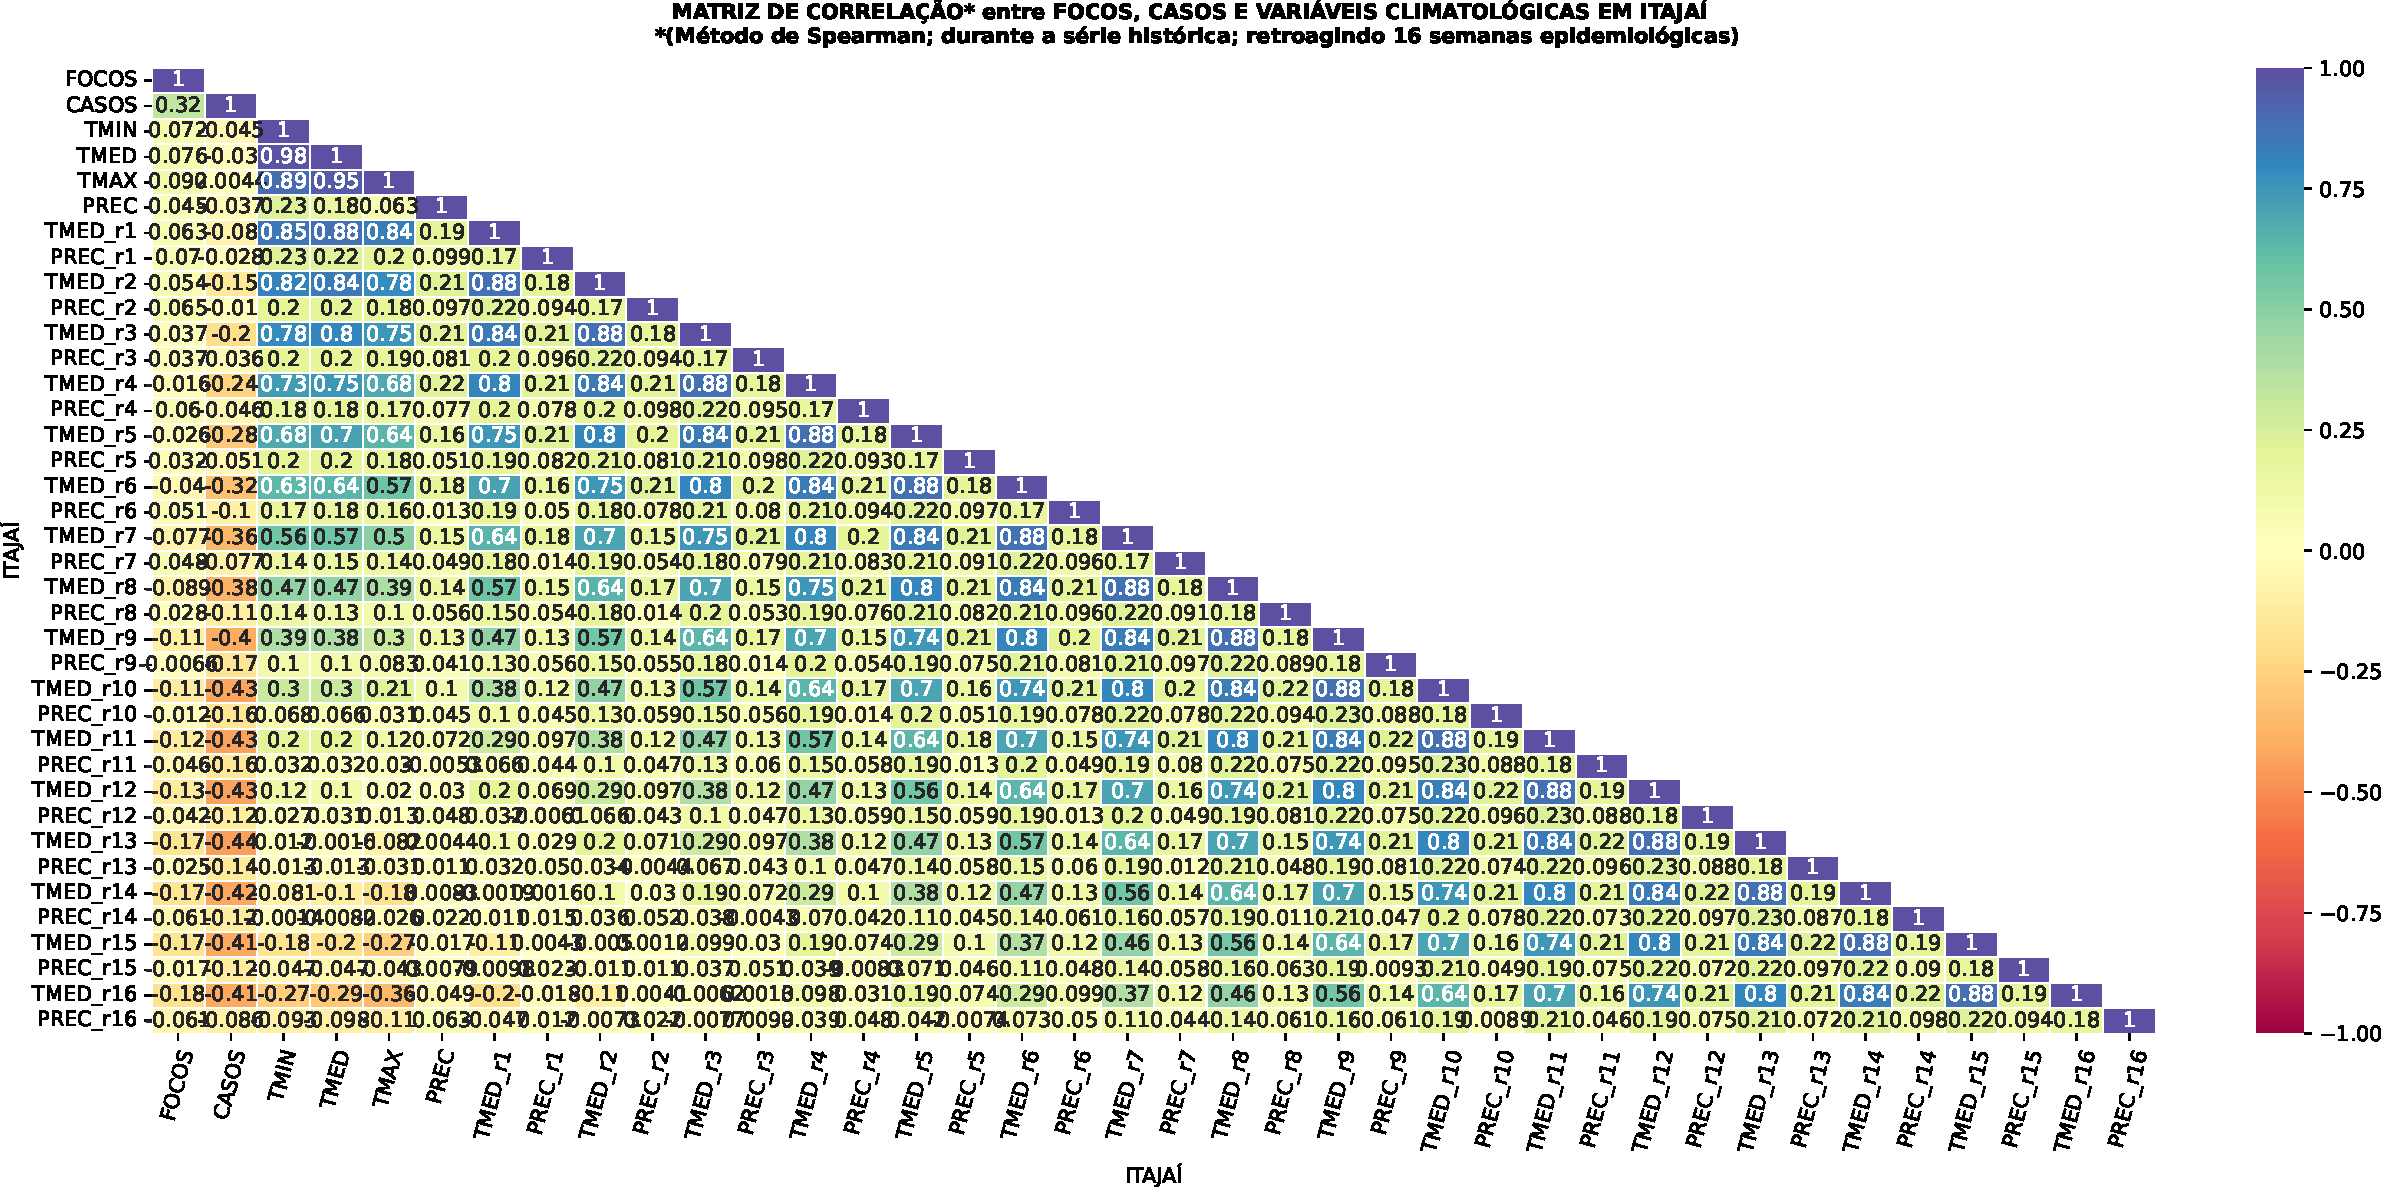
\includegraphics[width=0.47\textwidth]{figuras/matriz_correlacao_spearman_ITAJAI_r16s_total.pdf}
        }\hfill
    \subfloat[Joinville \label{fig: corr_CLI_JOItotal}]{
        \centering
        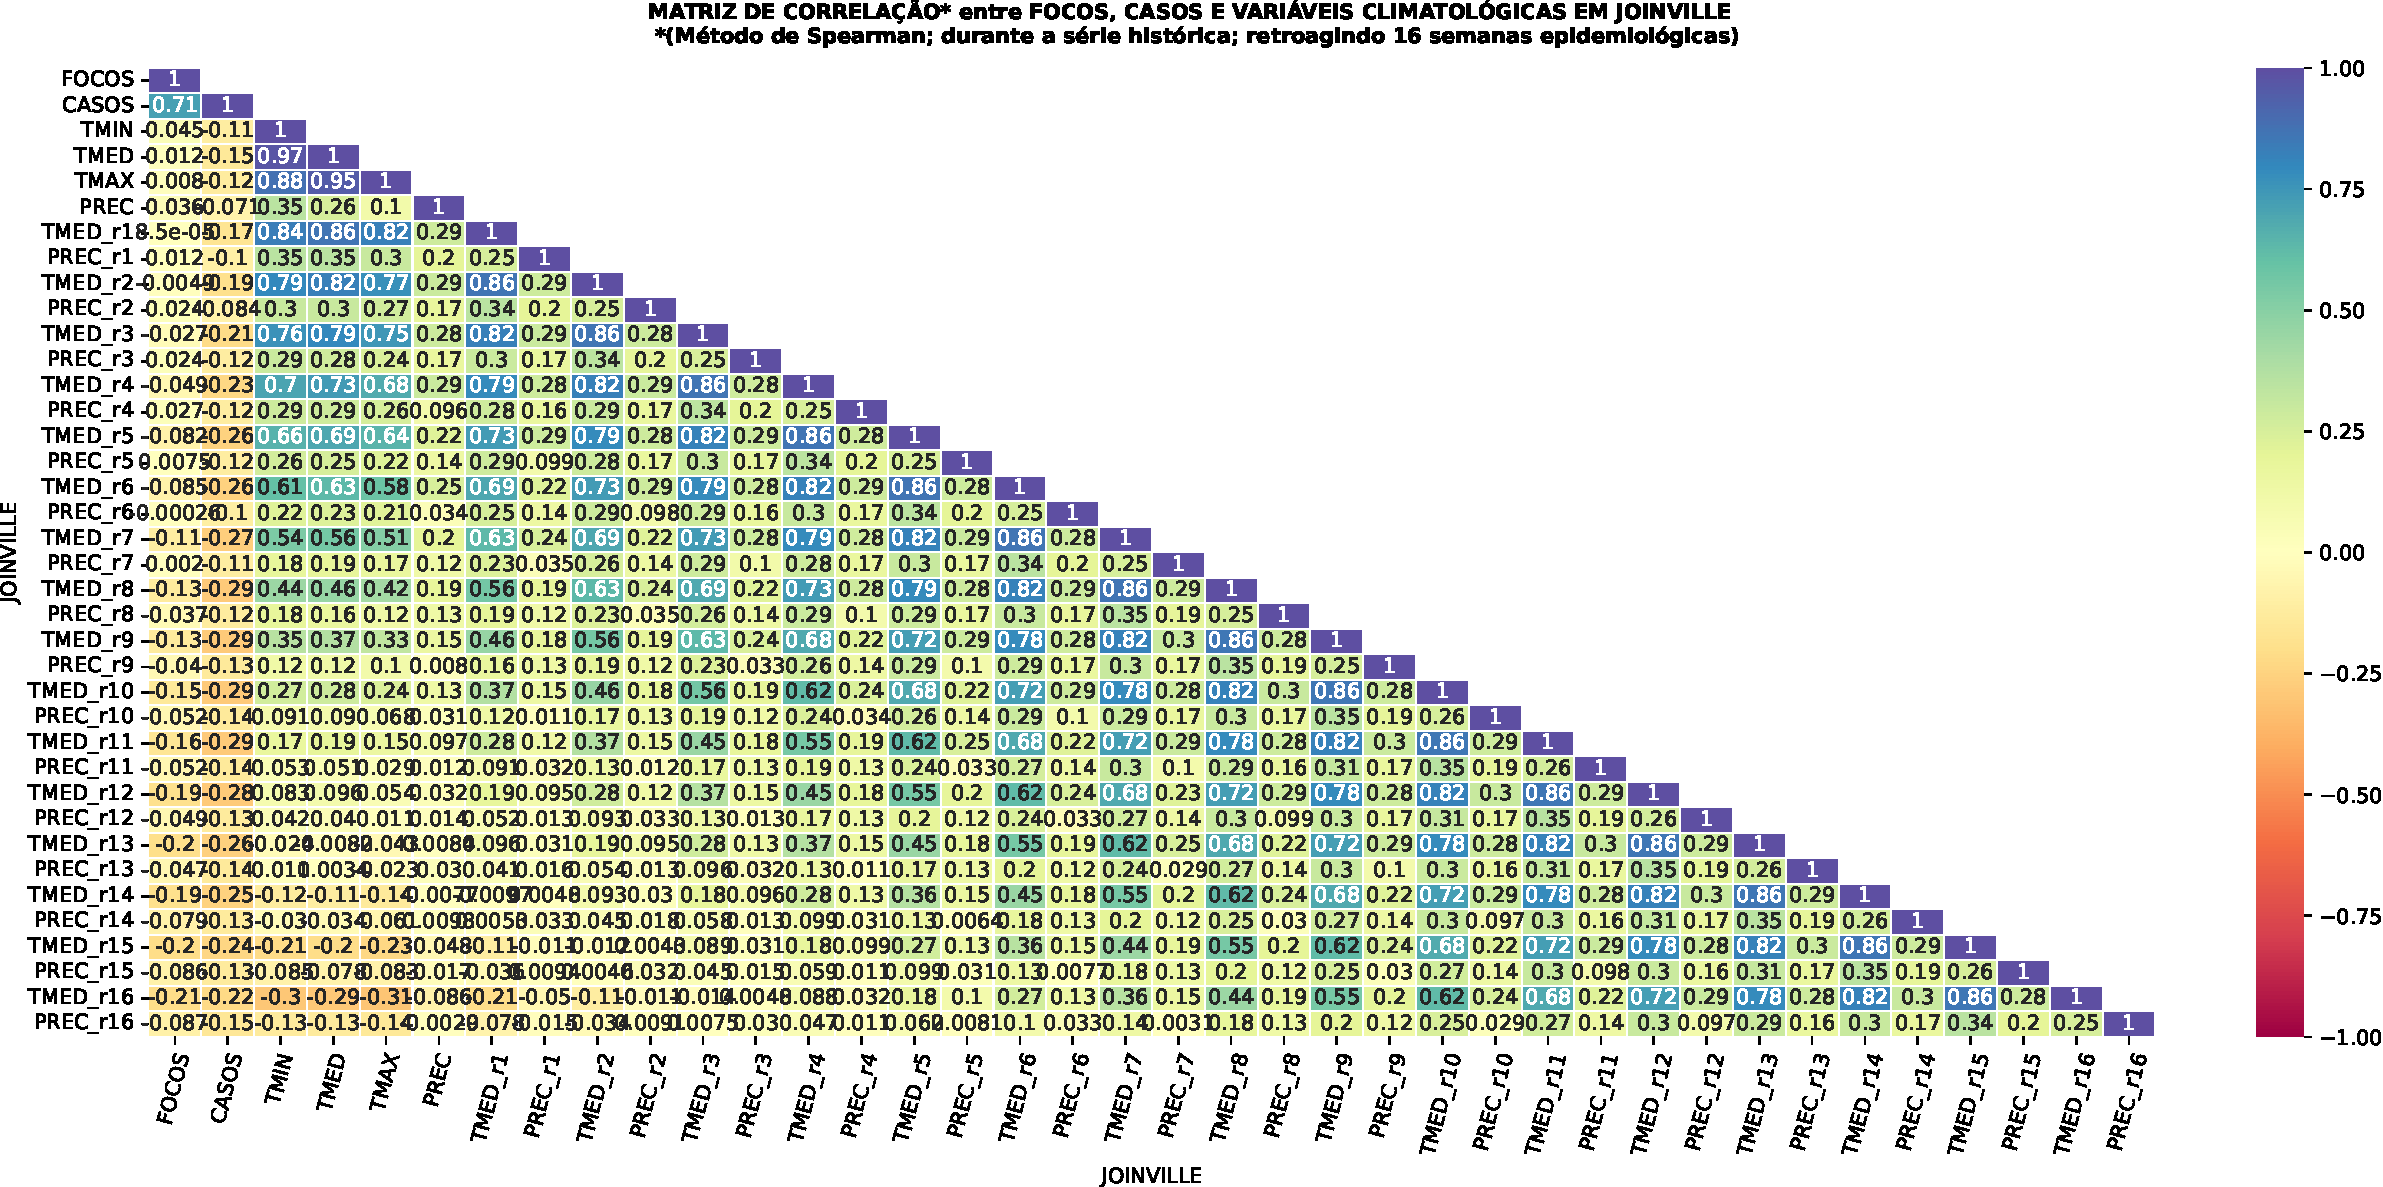
\includegraphics[width=0.47\textwidth]{figuras/matriz_correlacao_spearman_JOINVILLE_r16s_total.pdf}
        }
    \subfloat[Chapecó \label{fig: corr_CLI_CHAtotal}]{
        \centering
        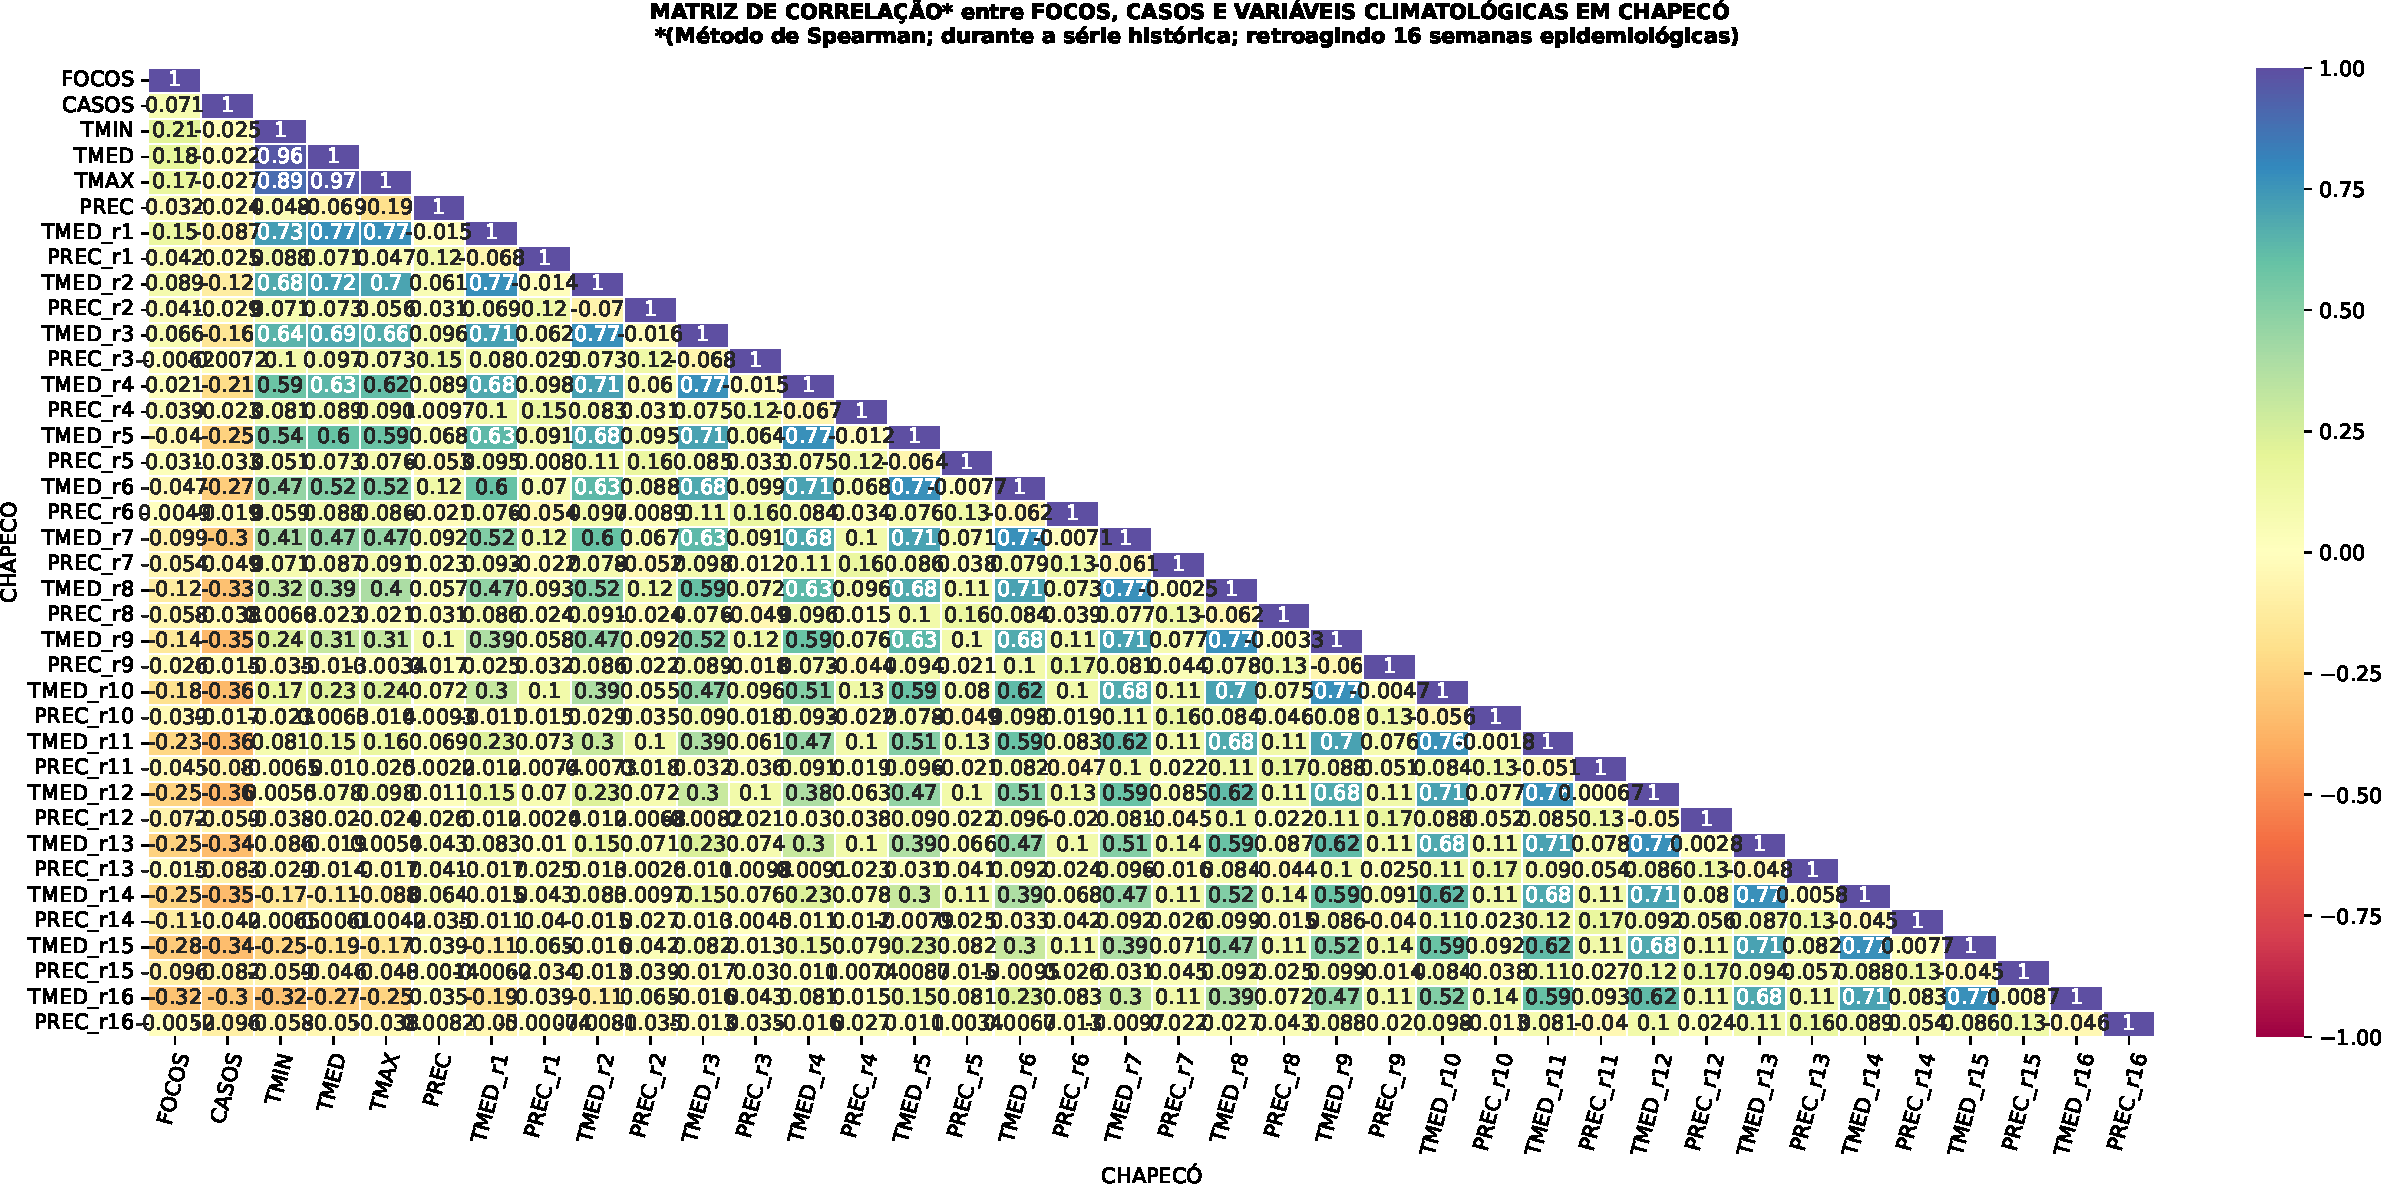
\includegraphics[width=0.47\textwidth]{figuras/matriz_correlacao_spearman_CHAPECO_r16s_total.pdf}
        }\hfill
    \end{center}
    \small{Fonte: Elaboração própria (2024).}
\end{figure}

% E entre os \acrshort{DEE} e limiares dos \acrshort{DEC}.
\indent Para lidar com as correlações de limiares climatológicos, aserá analisado cada cidade separada. Começando pela capital do Estado, Florianópolis (figura \ref{fig: matriz_corr_LIM_FLOretro}), e analisando o ano de 2023, pode-se verificar que as maiores correlações em relação aos focos de \latim{Aedes} sp. ocorreram retrocedendo uma (1) semana epidemiológica (figura \ref{fig: corr_LIM_FLOretro1s}), em temperaturas máximas amenas. \textcolor{red}{Uma possível explicação é essa temperatura máxima amena ser uma faixa de conforto para o pernilongo, como demonstrando em outros estudos.} Enquanto as maiores intensidades de correlações, mesmo nagativas, em relação aos casos de dengue ocorreram retrocedendo oito (8) semanas epidemiológicas (figura \ref{fig: corr_LIM_FLOretro8s}), em temperaturas mínimas e máximas moderadas, diminuindo a intensidade nos extremos. \textcolor{red}{Sugere-se o atraso por conta do tempo de incubação intrínsico. As temperaturas máxima e mínima aparentam faixas de temperaturas ótimas para a biologia do vetor, além de que os extremos para ambas as temperaturas podem estar ligados também ao comportamento humano, como no decréscimo das temperaturas, diminuir atividades ao ar livre e utilizar roupas que cubram mais o corpo.}

\begin{figure}[htbp]
    \begin{center}
    \caption{Matriz de correlações entre focos de \latim{Aedes} sp., casos de dengue e limiares de variáveis climatológicas em Florianópolis, durante o ano de 2023 retrocedendo semanas epidemiológicas, método de Spearman.}
    \label{fig: matriz_corr_LIM_FLOretro}
    \subfloat[Uma semana epidemiológica \label{fig: corr_LIM_FLOretro1s}]{
        \centering
        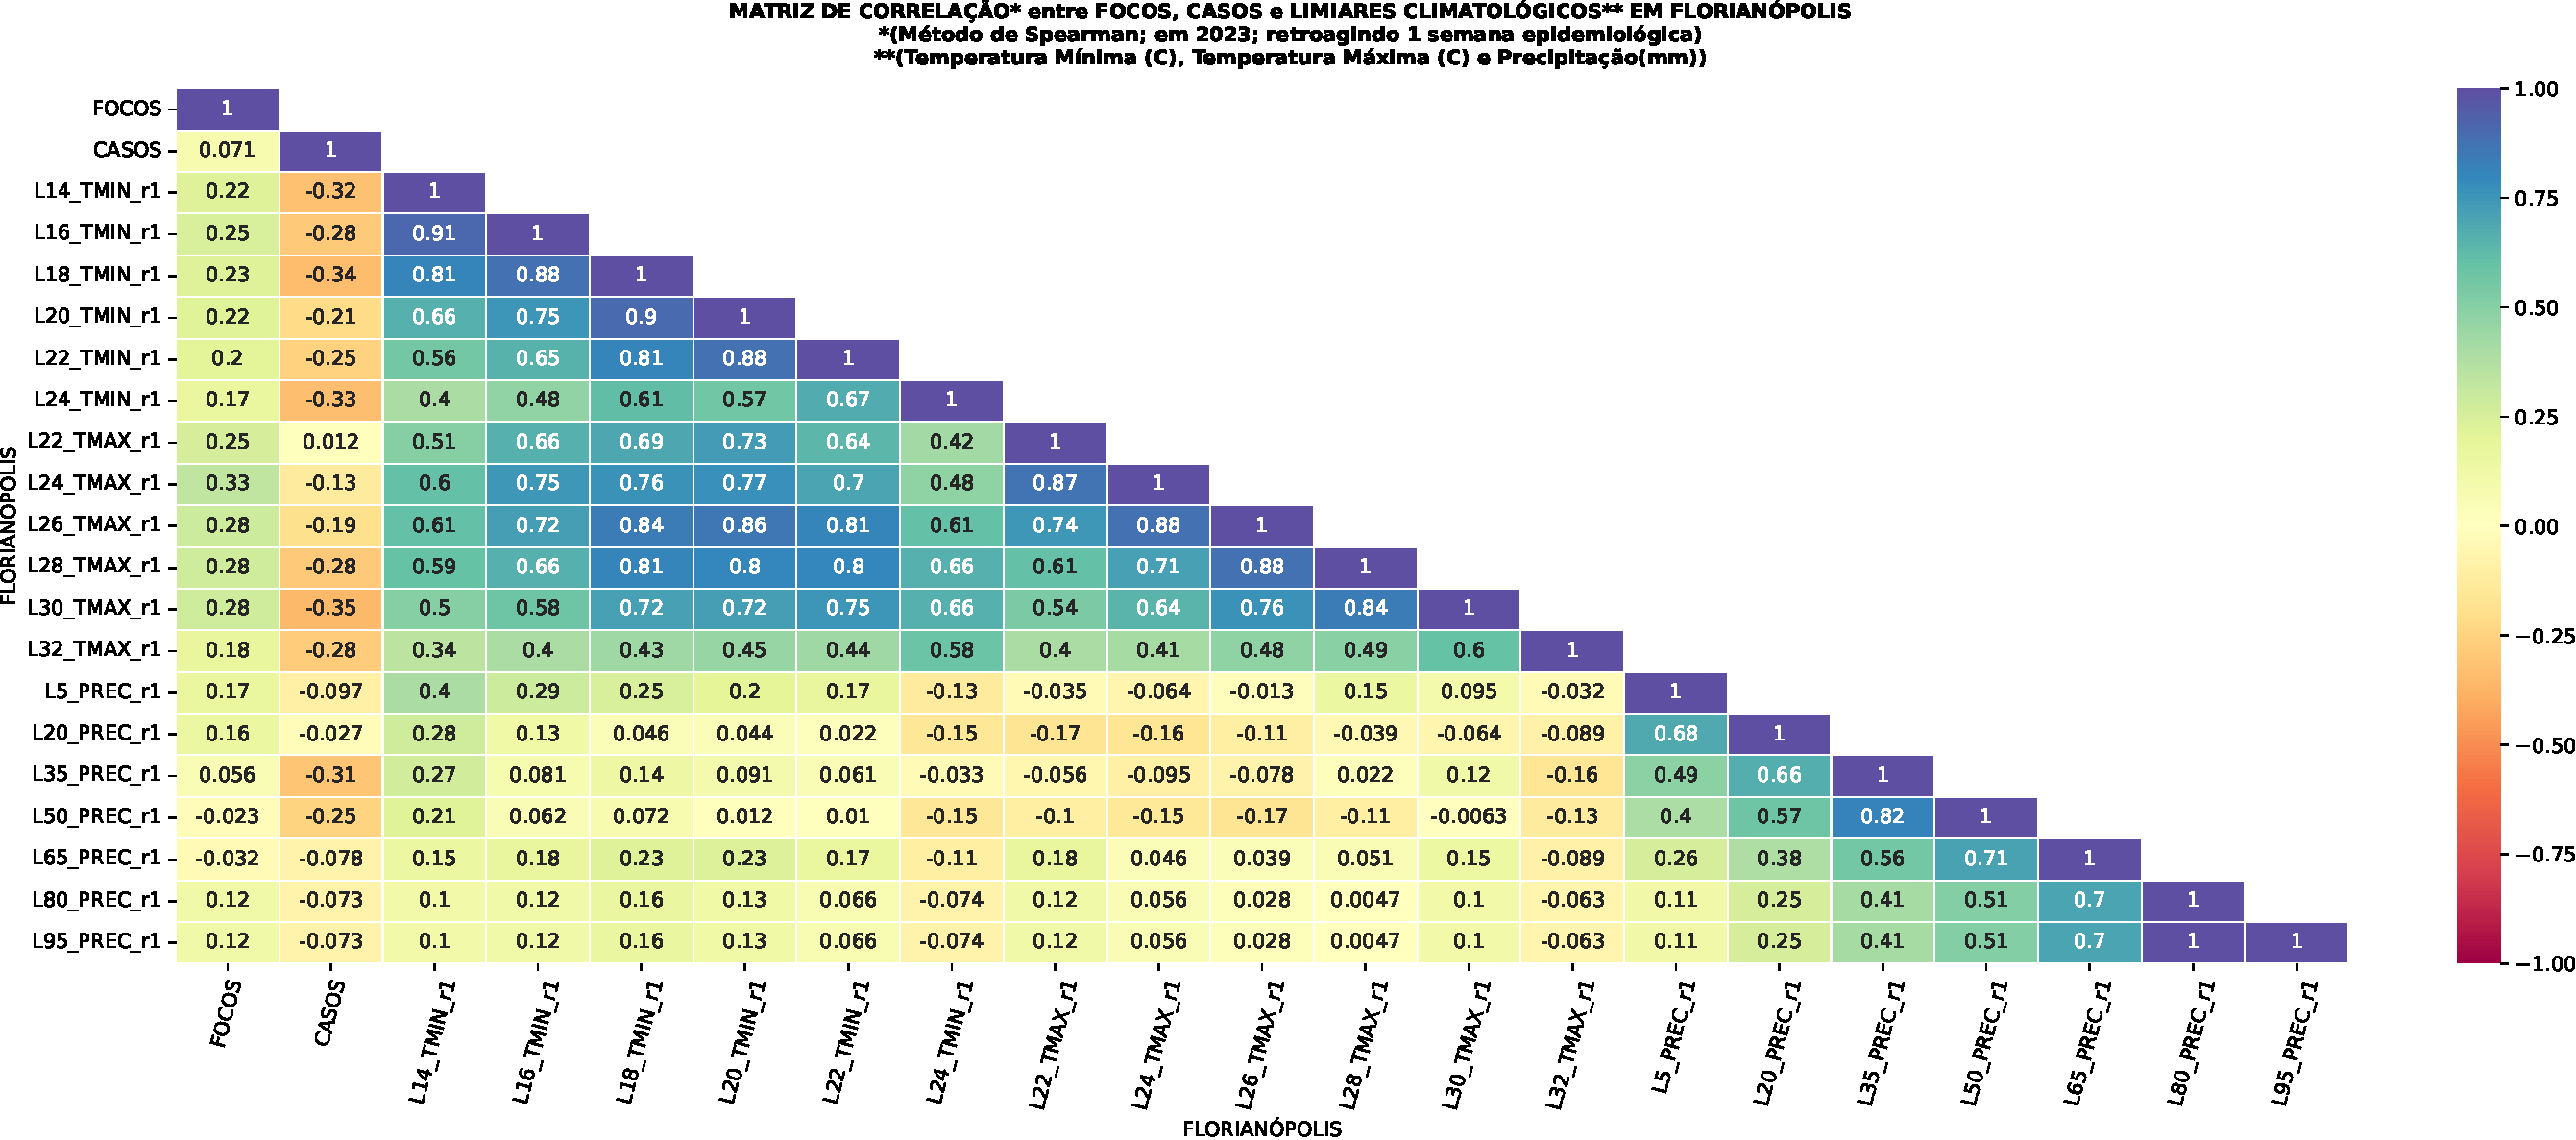
\includegraphics[width=0.47\textwidth]{figuras/matriz_correlacao_spearman_retrolimiar_FLORIANOPOLIS_2023_r1s.pdf}
        }
    \subfloat[Oito semanas epidemiológicas \label{fig: corr_LIM_FLOretro8s}]{
        \centering
        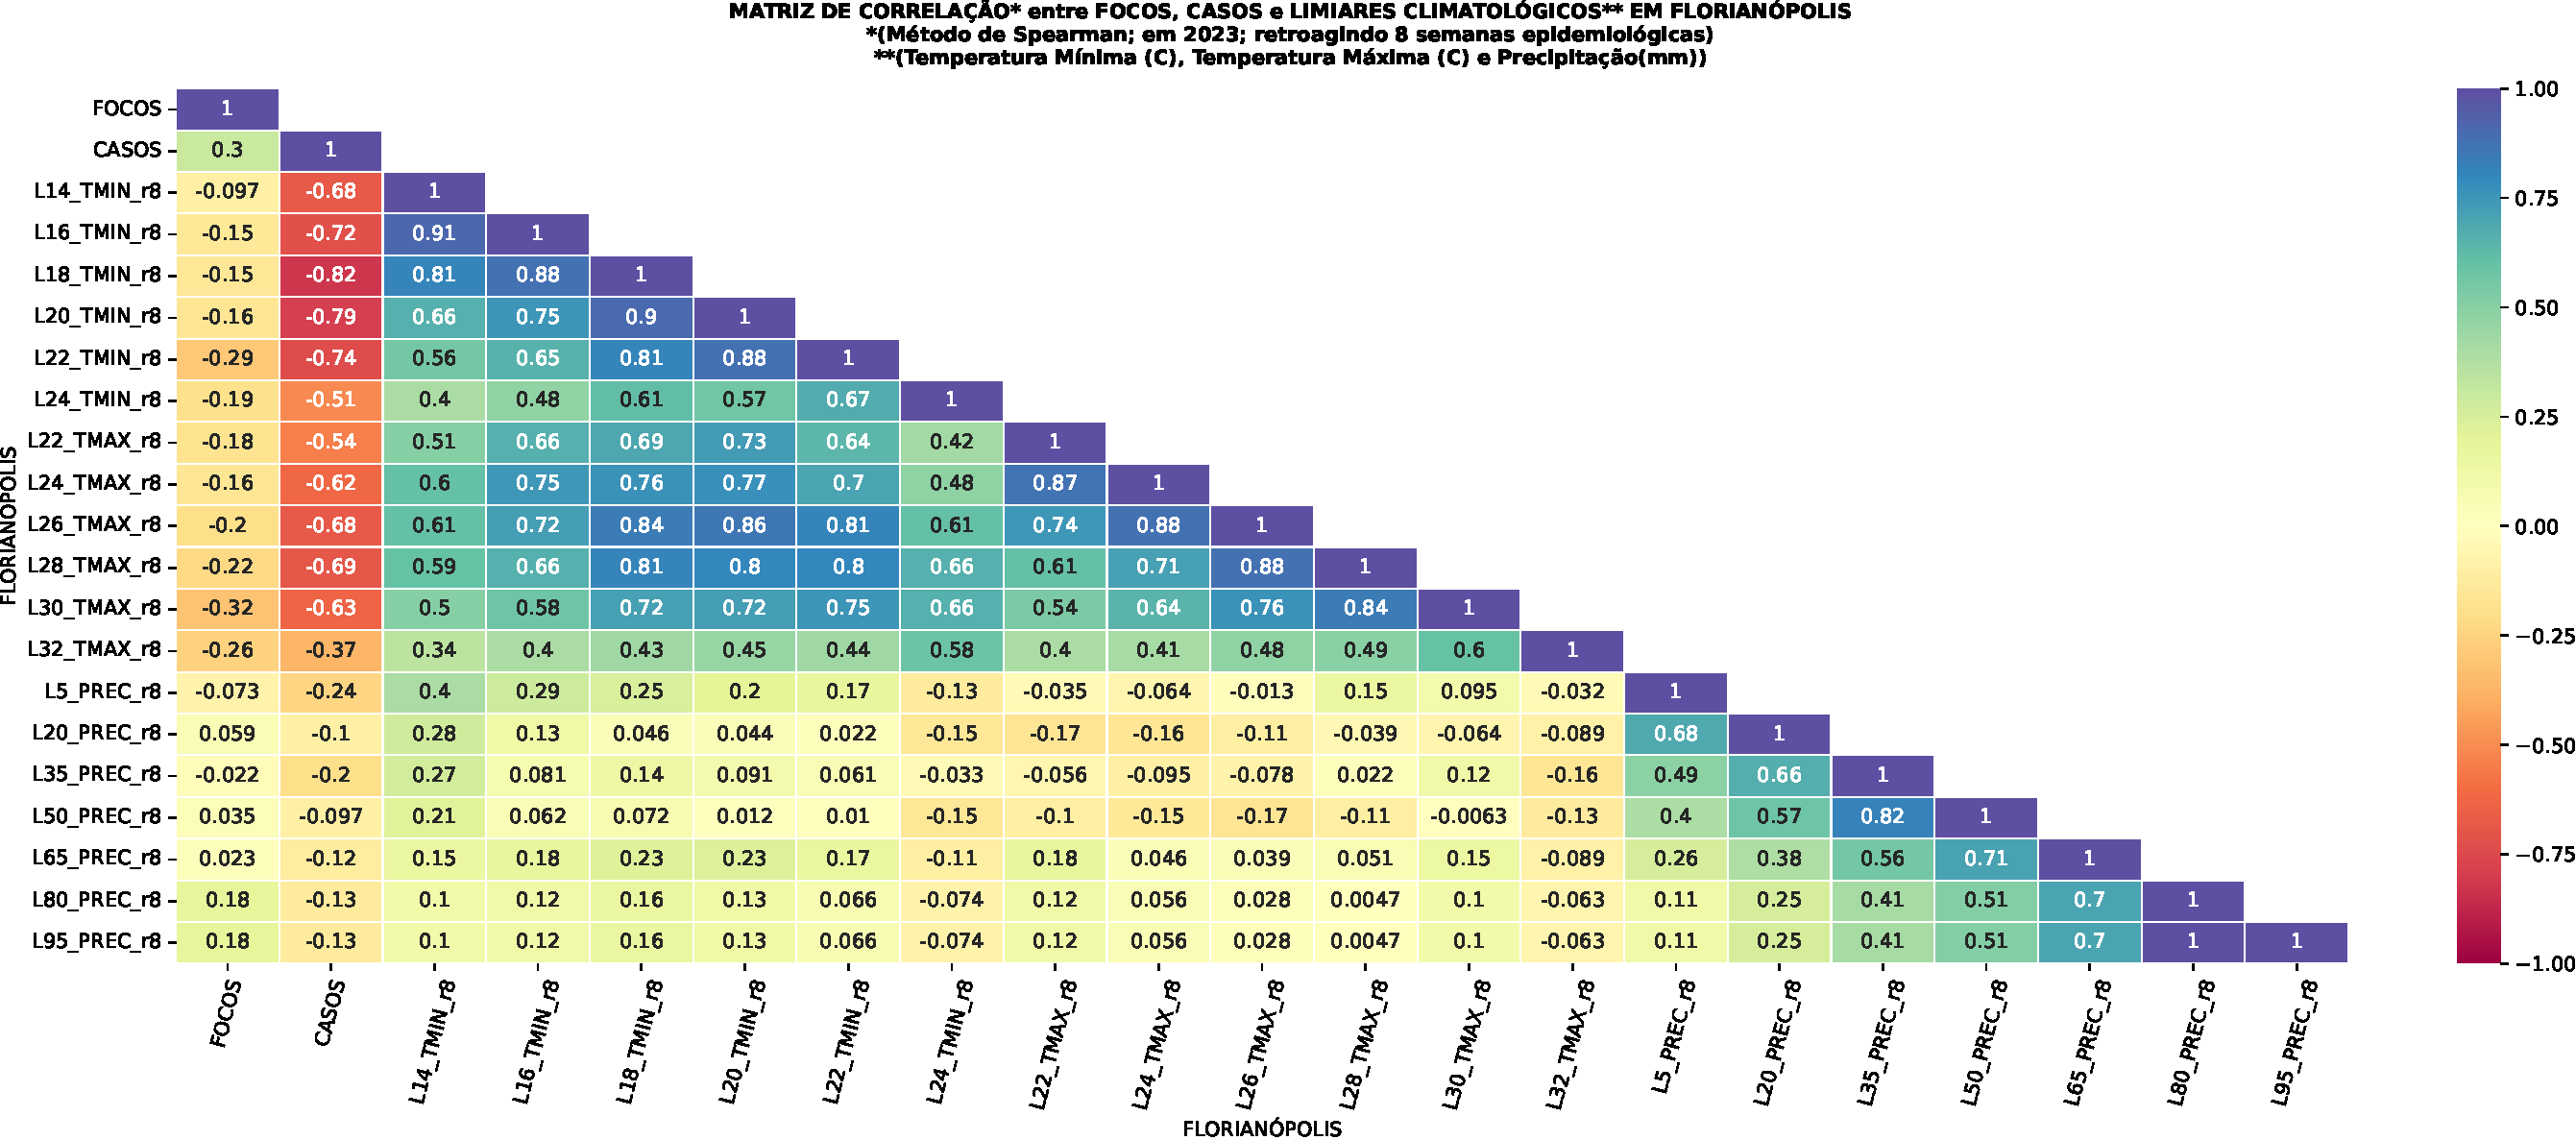
\includegraphics[width=0.47\textwidth]{figuras/matriz_correlacao_spearman_retrolimiar_FLORIANOPOLIS_2023_r8s.pdf}
        }
        \hfill
    \end{center}
    \small{Fonte: Elaboração própria (2024).}
\end{figure}

Ainda, analisando as correlações entre focos de \latim{Aedes} sp. e precipitação a partir de limiares em Florianópolis (figura \ref{fig: matriz_corr_LIMprec_FLO}), pode-se verificar correlação média positiva acima do limiar de 5 mm quando retrocedido duas (2) semanas epidemiológicas (figura \ref{fig: corr_LIMprec_FLO5lim}). Quando não se retrocede ou apenas retrocede uma (1) semana epidemiológica, verifica-se correlações baixas positivas nesse mesmo limiar. Essas correlações ficam oscilando entre limiares e essas mesmas semanas retroagidas, até atingirem o valor maior no limiar de 30 mm, quando se verifica correlação média positiva retrocedendo uma (1) semana epidemiológica nesse limiar (figura \ref{fig: corr_LIMprec_FLO30lim}). Após o limiar de 35 mm, as correlações reduzem para baixas ou inexistentes. \textcolor{red}{Biologia do vetor que tende a baixos volumes de precipitação e não muito retroativo.}

\begin{figure}[htbp]
    \begin{center}
    \caption{Matriz de correlações entre focos de \latim{Aedes} sp., casos de dengue e limiares de precipitação (mm) em Florianópolis, durante o ano de 2023 retrocedendo semanas epidemiológicas, método de Spearman.}
    \label{fig: matriz_corr_LIMprec_FLO}
    \subfloat[Limiar - 5 mm \label{fig: corr_LIMprec_FLO5lim}]{
        \centering
        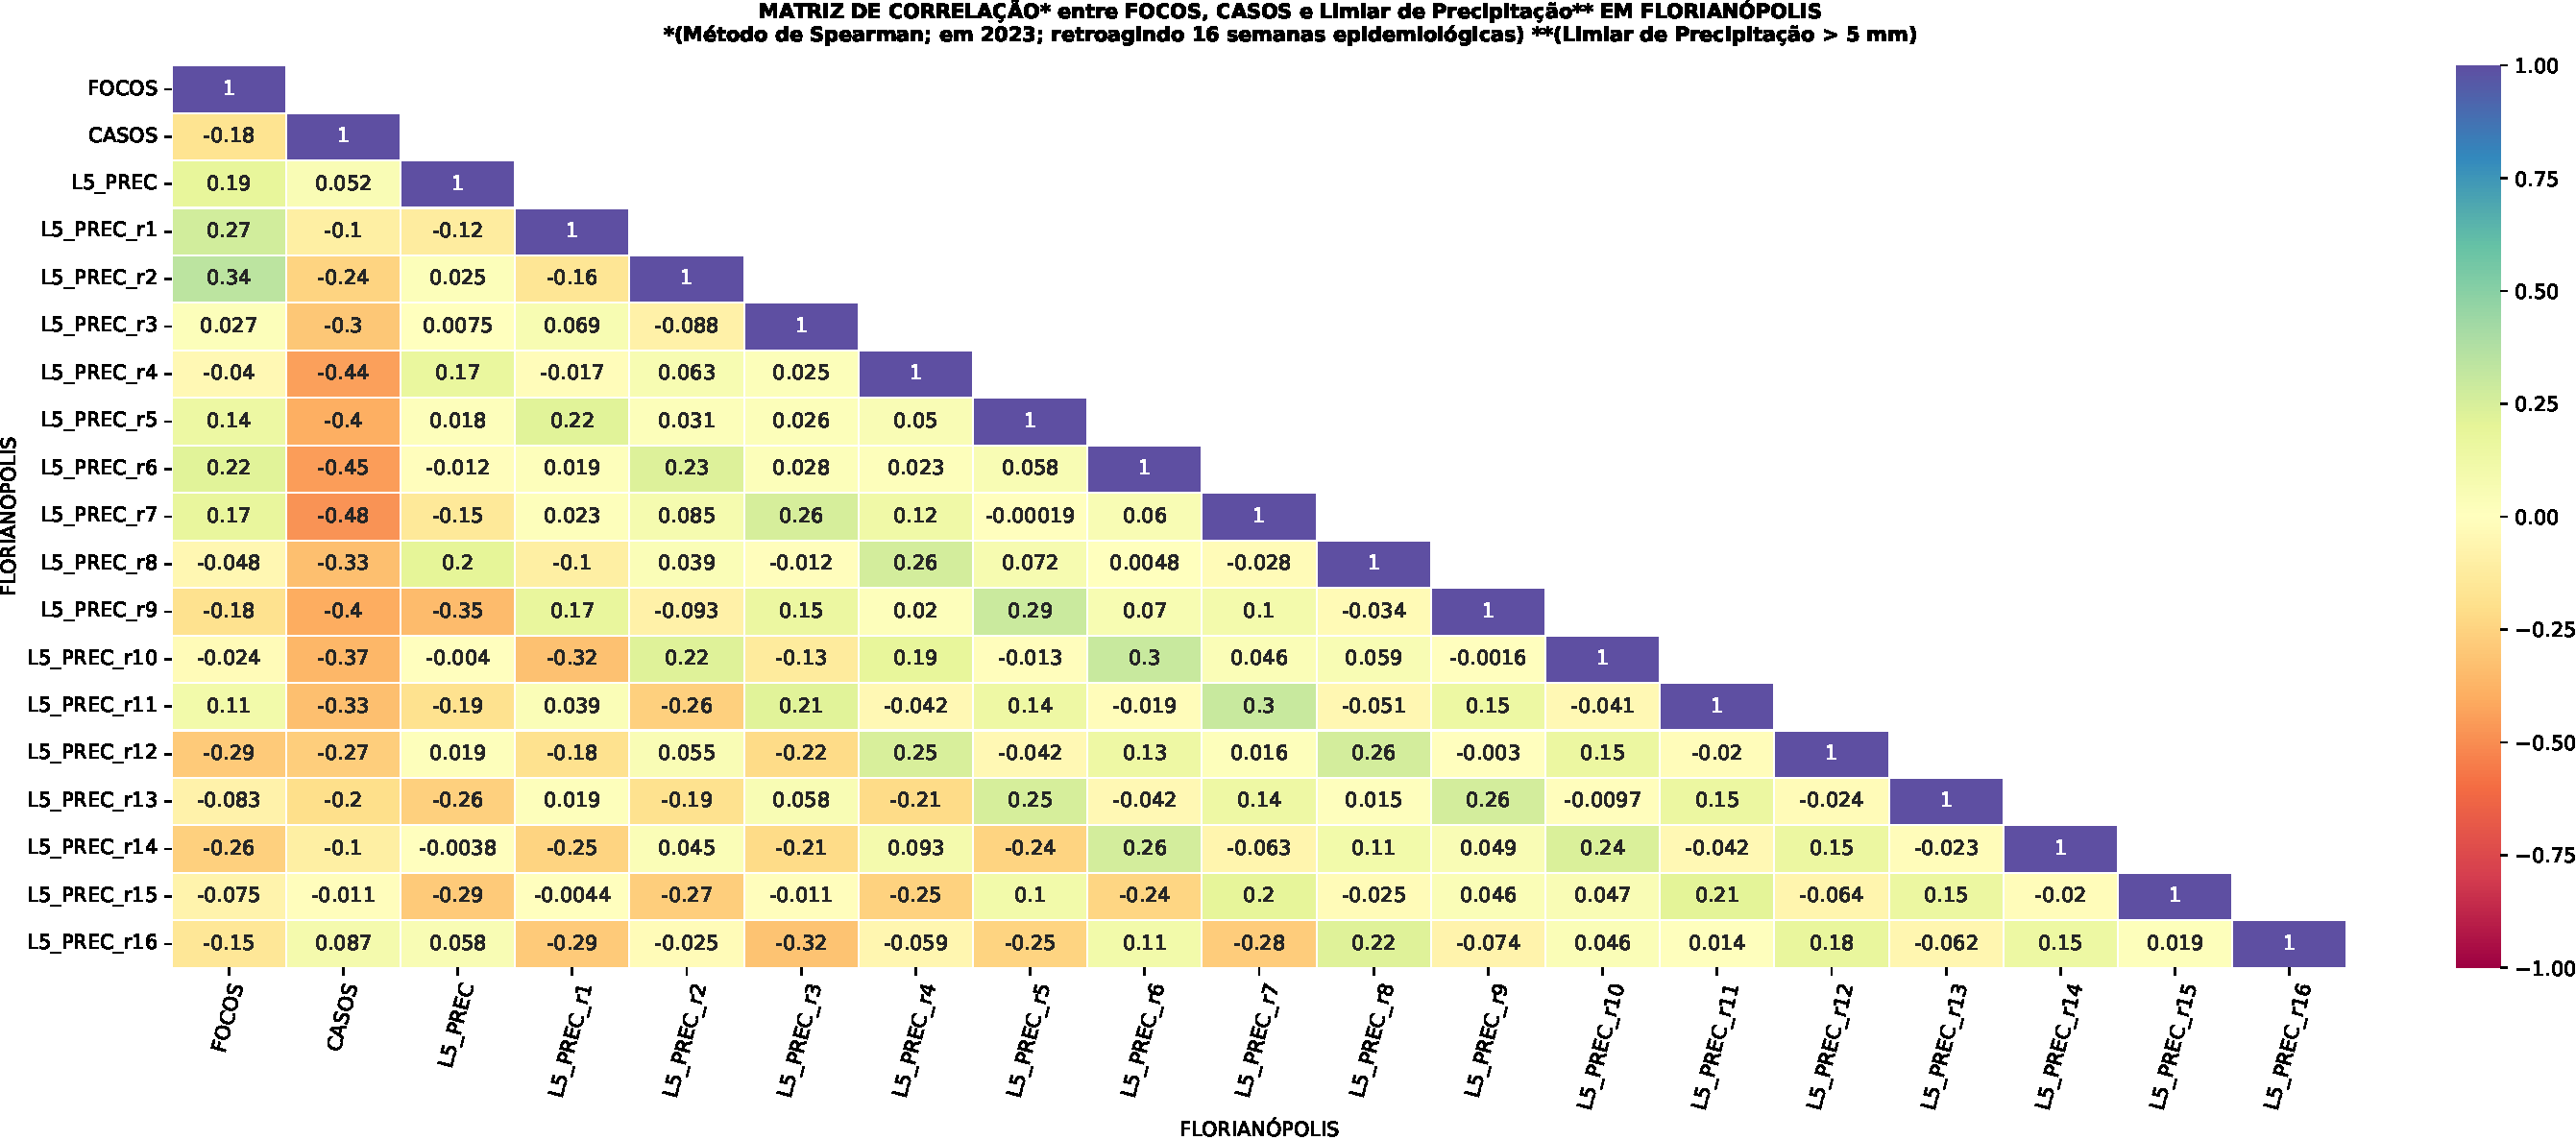
\includegraphics[width=0.47\textwidth]{figuras/matriz_correlacao_spearman_prec_FLORIANOPOLIS_r16s_2023_LIMIAR5.pdf}
        }
    \subfloat[Limiar - 30 mm \label{fig: corr_LIMprec_FLO30lim}]{
        \centering
        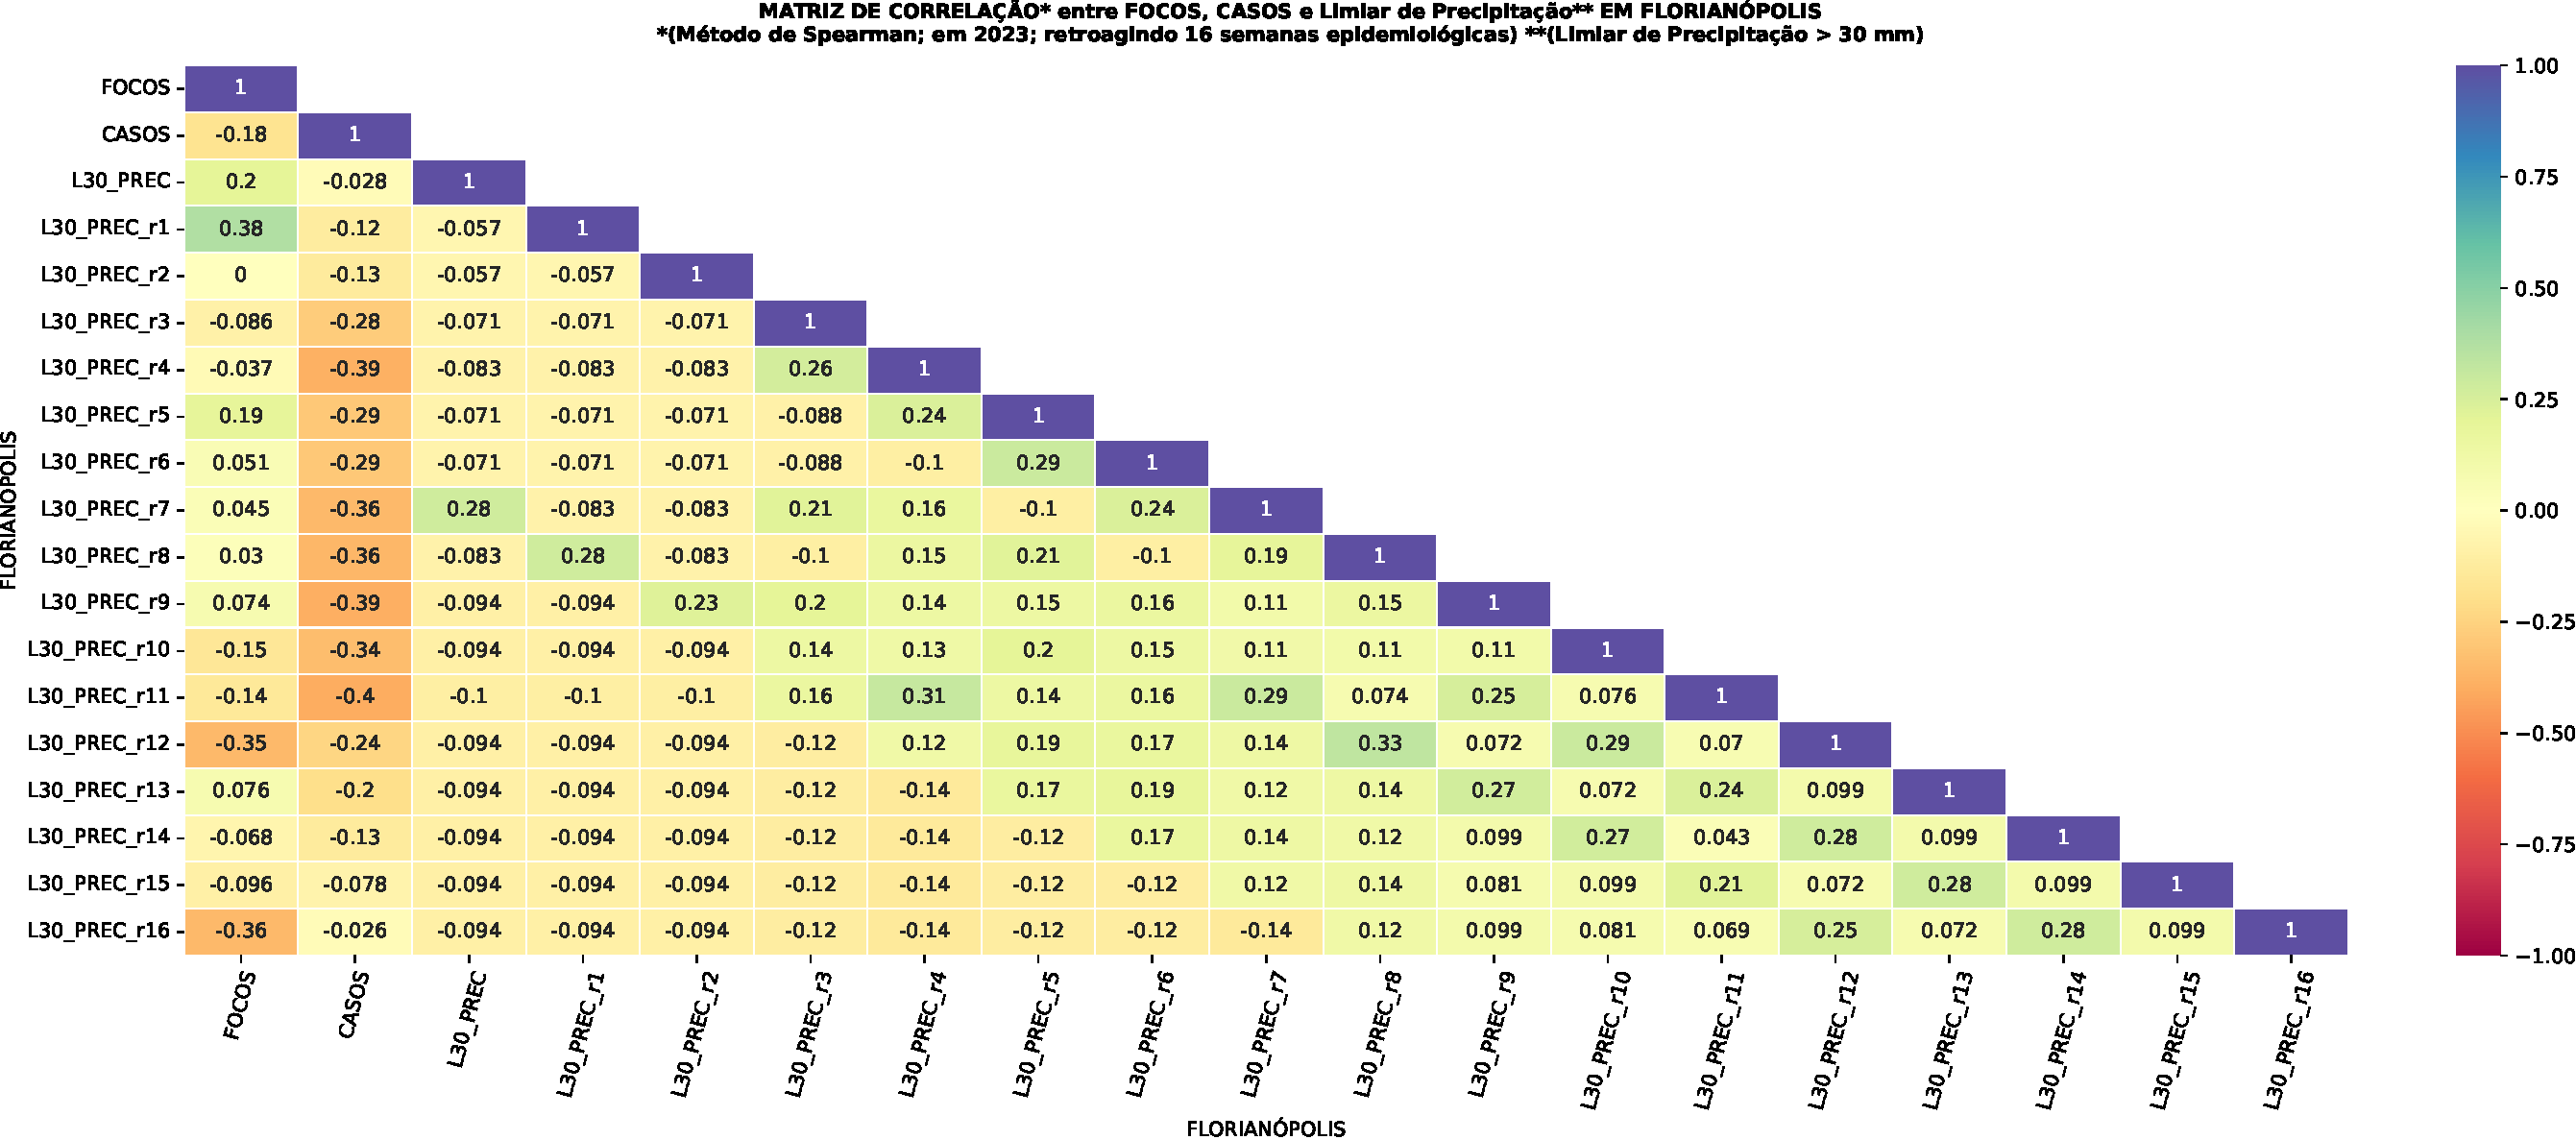
\includegraphics[width=0.47\textwidth]{figuras/matriz_correlacao_spearman_prec_FLORIANOPOLIS_r16s_2023_LIMIAR30.pdf}
        }
        \hfill
    \end{center}
    \small{Fonte: Elaboração própria (2024).}
\end{figure}

\indent Adicionalmente, analisando as correlações entre temperatura mínima e variáveis entomo-epidemiológicas em Florianópolis (figura \ref{fig: matriz_corr_LIMtmin_FLO}), percebe-se alguns padrões. Ao se analisar temperaturas acima do limiar de 14 C (figura \ref{fig: corr_LIMtmin_FLO14lim}), tem-se correlações que intensificam entre os casos de dengue, negativamente, quando retroagidos até certo tempo e perdem intensidade ao prosseguir a retroação. Além de que, correlacionando limiar de 14 C da temperatura mínima e focos de \latim{Aedes} sp., tem-se correlação média positiva ao retroceder uma (1) e cinco (5) semanas epidemiológicas, entre esses períodos as correlações perdem intensidade. \textcolor{red}{Discutir.} Em relação ao limiar de 24 C na temperatura mínima (figura \ref{fig: corr_LIMtmin_FLO24lim}), tem-se padrão de oscilação das correlações entre focos de \latim{Aedes} sp., que variam entre média positiva a ausente ao passo que o tempo retrocede. Temperatura acima desse mesmo limiar, 24 C, correlacionada entre os casos dengue não apresentou grande oscilação, mantendo-se em correlação média negativa praticamente todos as semanas epidemiológicas. \textcolor{red}{Discutir.}

\begin{figure}[htbp]
    \begin{center}
    \caption{Matriz de correlações entre focos de \latim{Aedes} sp., casos de dengue e limiares de temperatura mínima (C) em Florianópolis, durante o ano de 2023 retrocedendo semanas epidemiológicas, método de Spearman.}
    \label{fig: matriz_corr_LIMtmin_FLO}
    \subfloat[Limiar - 14 C \label{fig: corr_LIMtmin_FLO14lim}]{
        \centering
        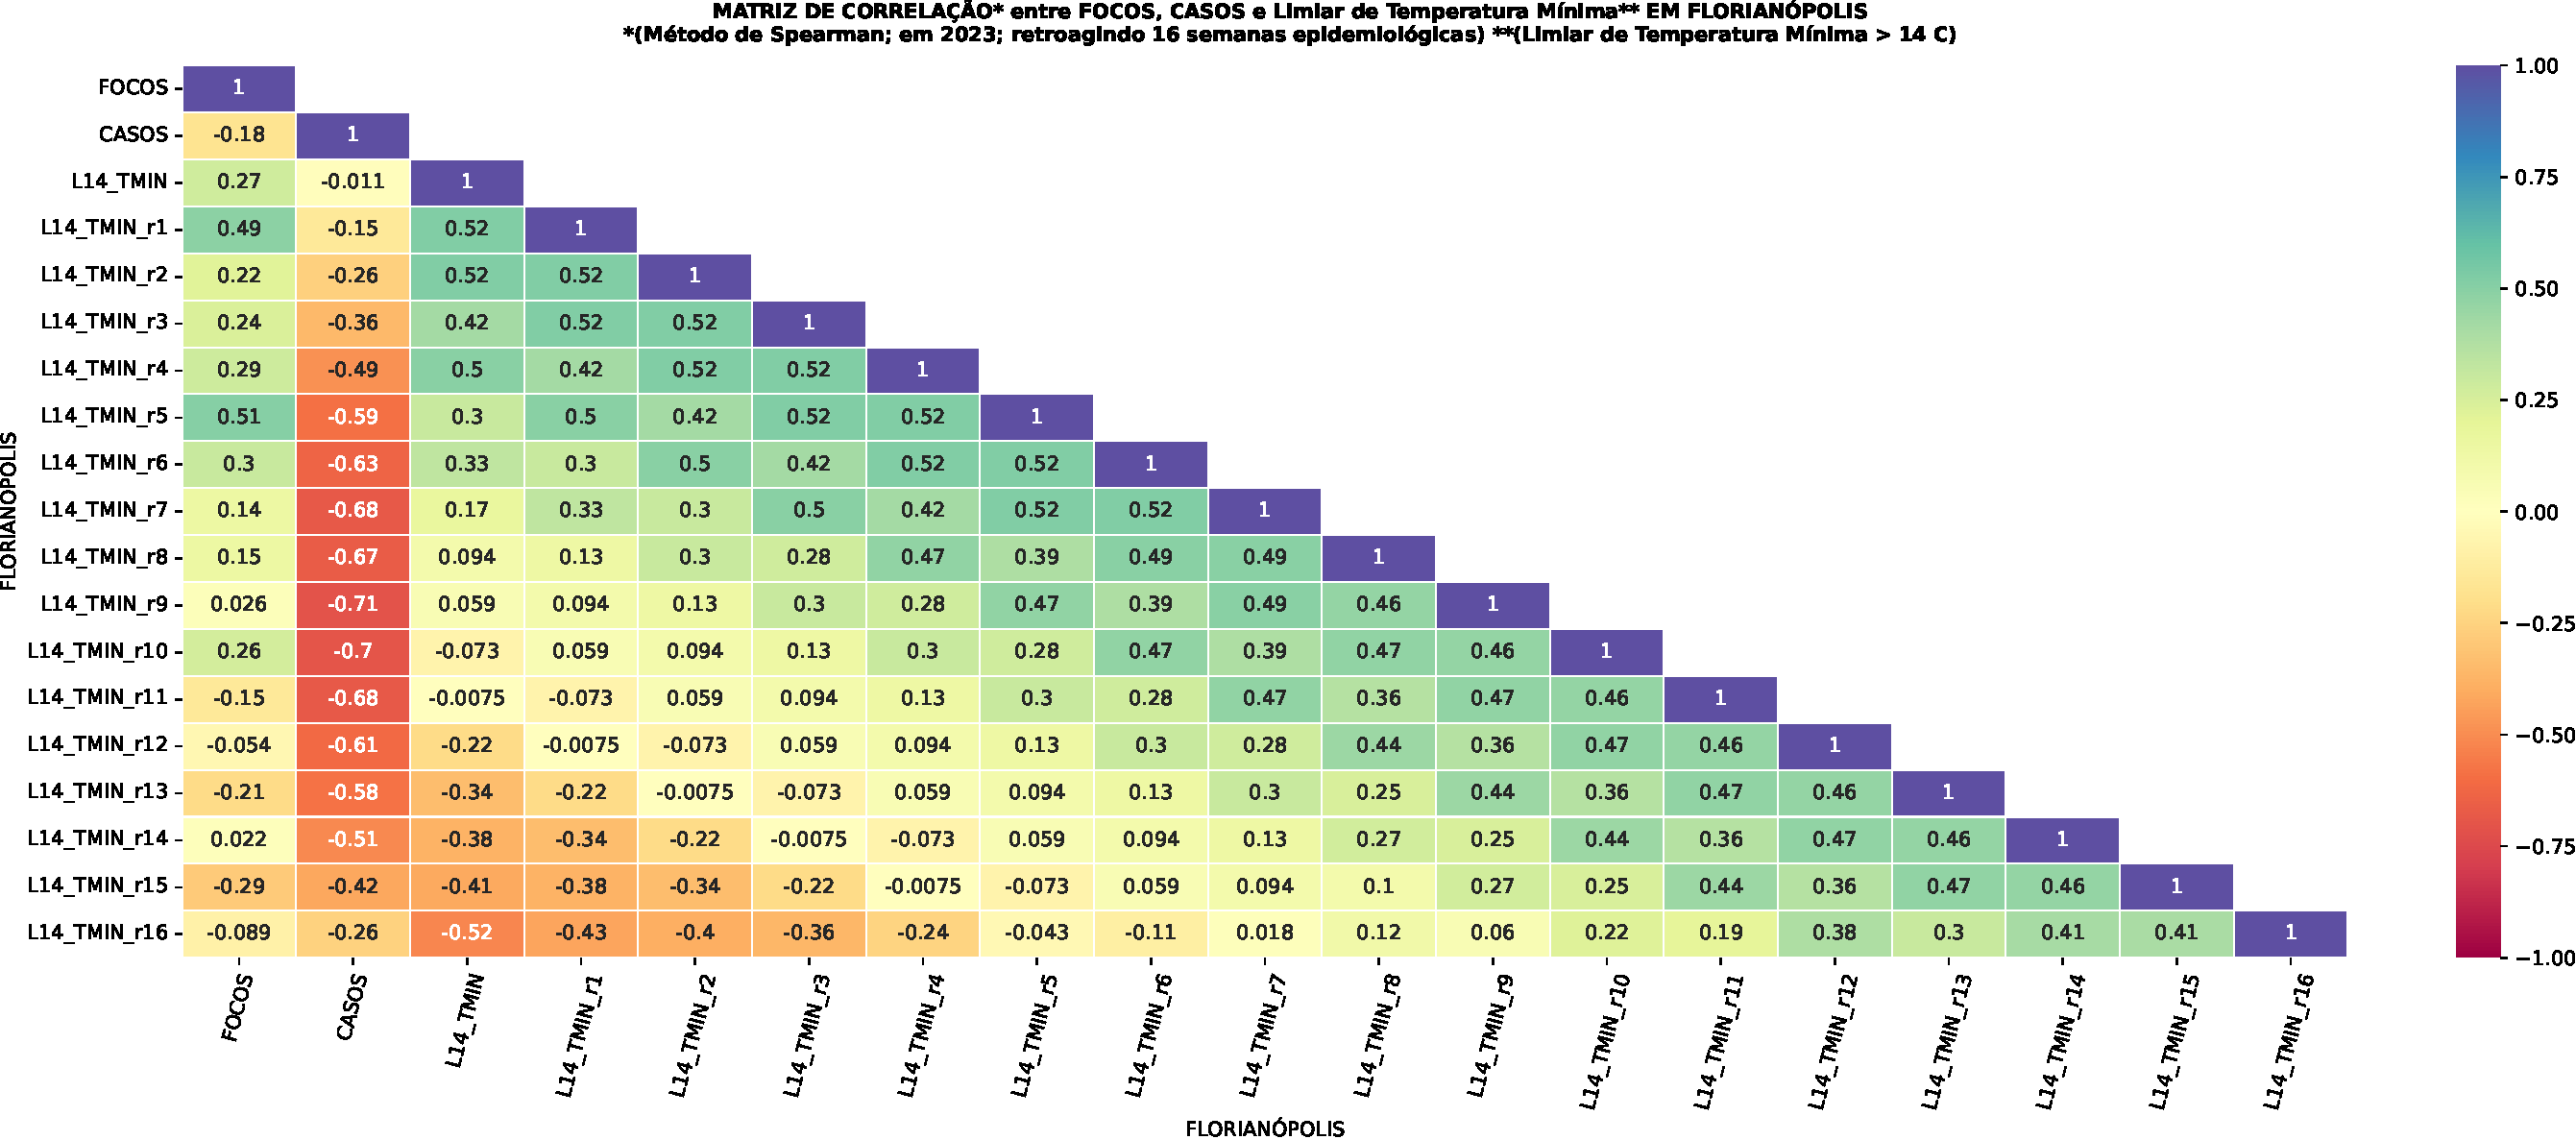
\includegraphics[width=0.47\textwidth]{figuras/matriz_correlacao_spearman_tmin_FLORIANOPOLIS_r16s_2023_LIMIAR14.pdf}
        }
    \subfloat[Limiar - 24 C \label{fig: corr_LIMtmin_FLO24lim}]{
        \centering
        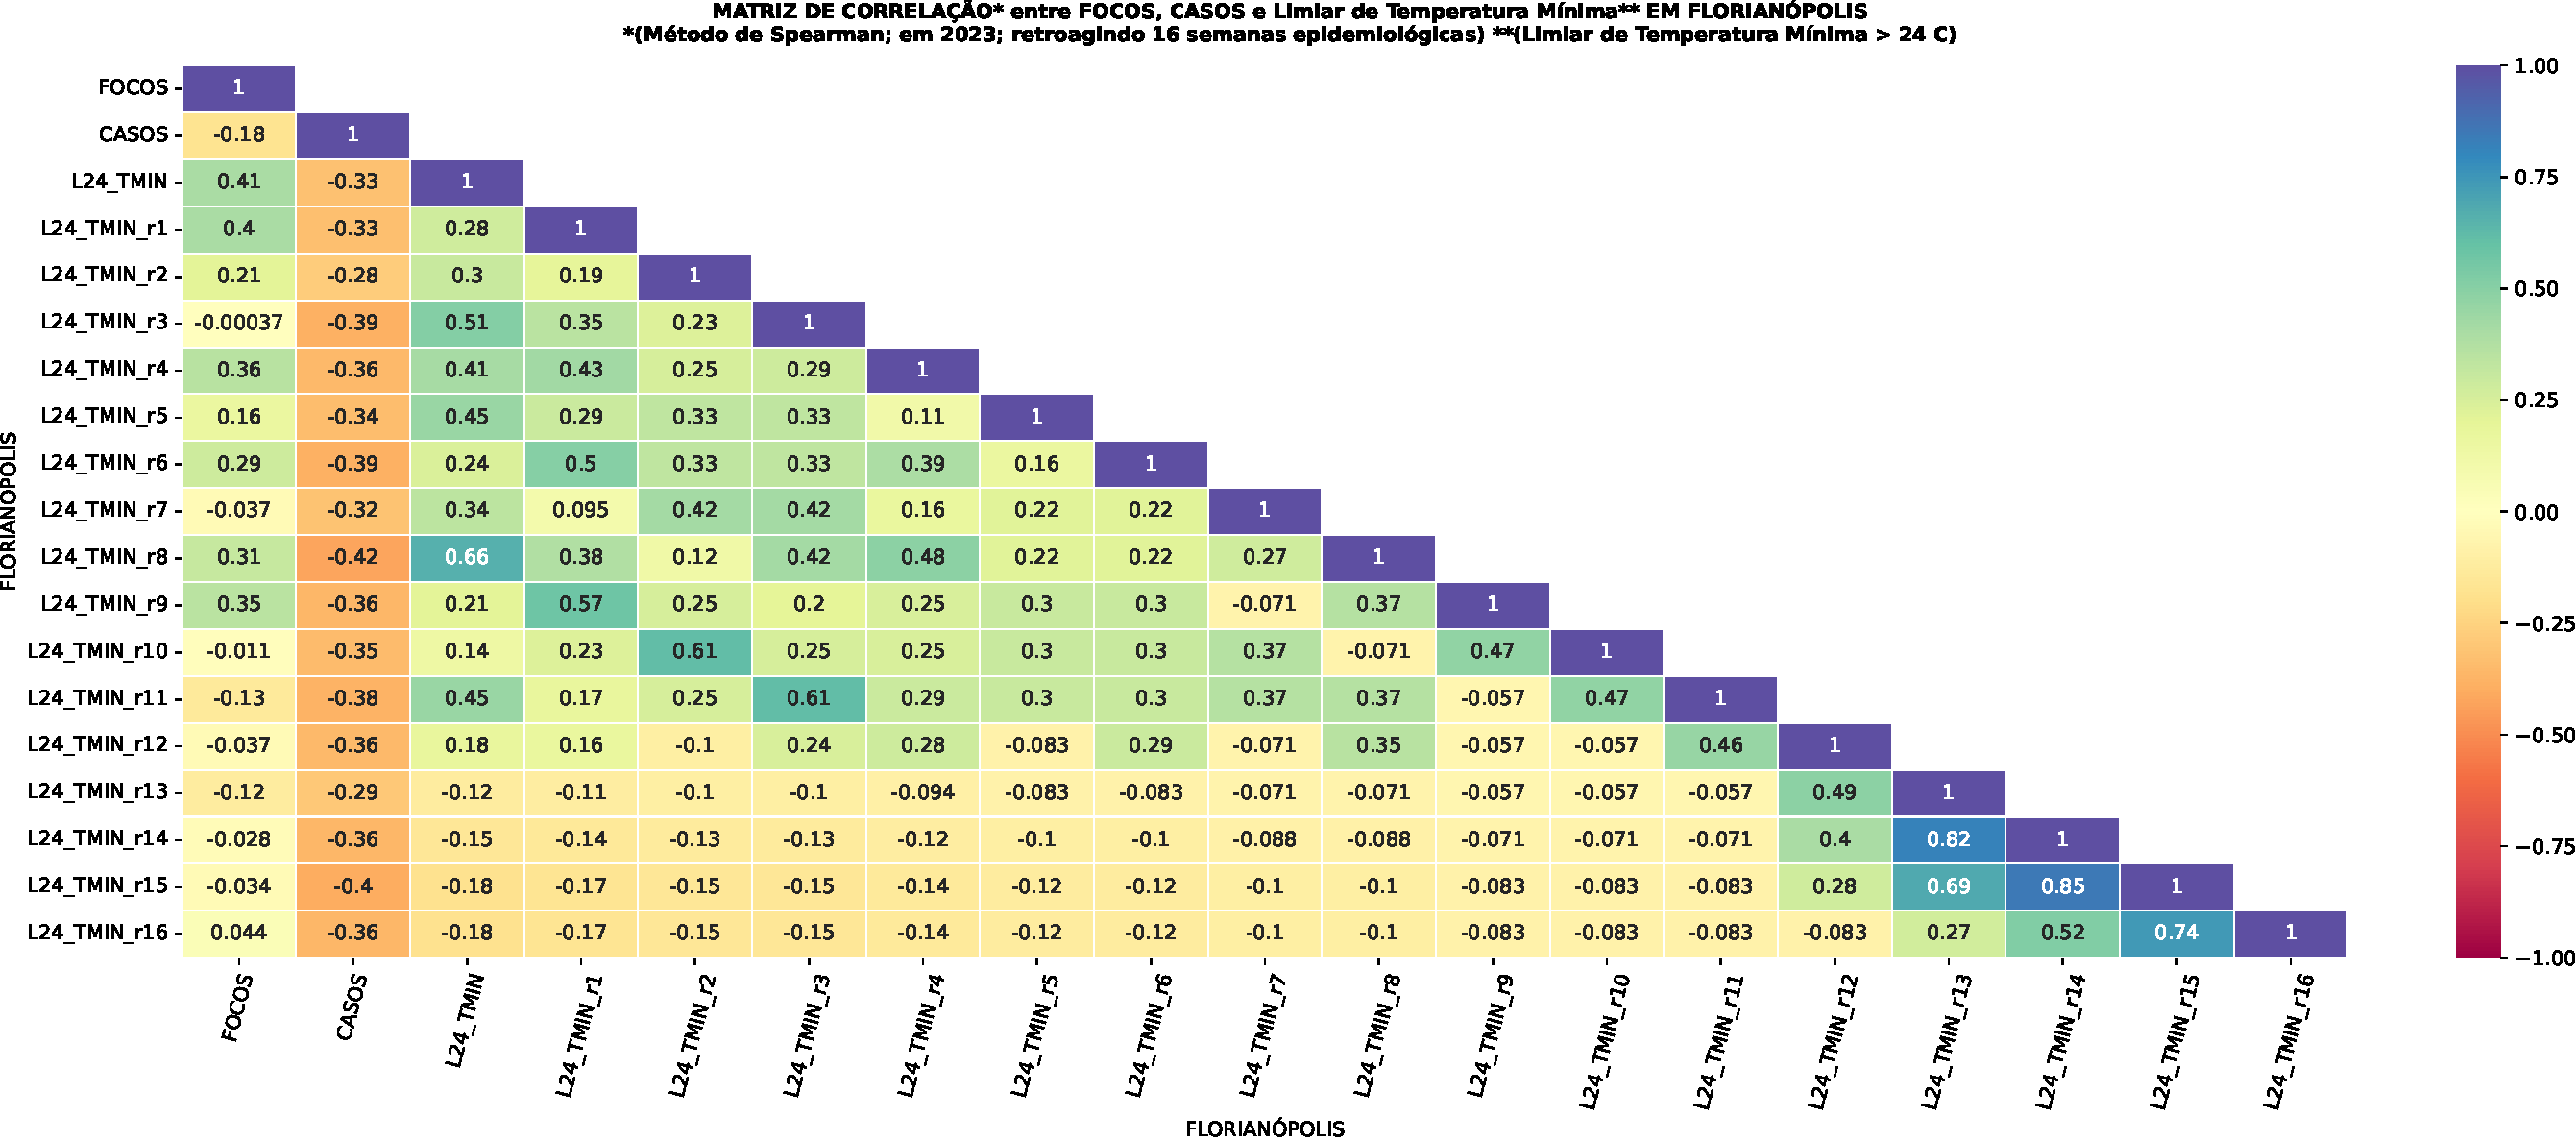
\includegraphics[width=0.47\textwidth]{figuras/matriz_correlacao_spearman_tmin_FLORIANOPOLIS_r16s_2023_LIMIAR24.pdf}
        }
        \hfill
    \end{center}
    \small{Fonte: Elaboração própria (2024).}
\end{figure}

\indent Igualmente, analisando as correlações entre temperatura máxima e variáveis entomo-epidemiológicas em Florianópolis (figura \ref{fig: matriz_corr_LIMtmax_FLO}), percebe-se que temperaturas abaixo do limiar de 22 C (figura \ref{fig: corr_LIMtmax_FLO22lim}), tem-se correlações que intensificam entre os casos de dengue, negativamente, quando retroagidos até certo tempo e perdem intensidade ao prosseguir a retroação. Além de que, correlacionando esse mesmo limiar da temperatura máxima, 22 C, e focos de \latim{Aedes} sp., tem-se correlações médias positivas oscilando entre baixas ou ausentes ao retroceder no tempo. Esses padrões de correlações, observados em focos de \latim{Aedes} sp. e casos de dengue no limiar de 22 C da temperatura máxima, são semelhantes aos observados no limiar de 14 C da temperatura mínima. \textcolor{red}{Discutir.} Sobre o limiar de 30 C da temperatura máxima (figura \ref{fig: corr_LIMtmax_FLO30lim}), correlações entre focos de \latim{Aedes} sp. apresentam intensidade média positiva na própria semana e retrocedendo uma (1) semana epidemiológica, perdendo intensidade enquanto retrocede. Correlacionando esse limiar e casos de dengue, correlações médias negativas são encontradas ao retroceder pouco no tempo, perdendo intensidade em tempos mais pretéritos. \textcolor{red}{Discutir.}

\begin{figure}[htbp]
    \begin{center}
    \caption{Matriz de correlações entre focos de \latim{Aedes} sp., casos de dengue e limiares de temperatura máxima (C) em Florianópolis, durante o ano de 2023 retrocedendo semanas epidemiológicas, método de Spearman.}
    \label{fig: matriz_corr_LIMtmax_FLO}
    \subfloat[Limiar - 22 C \label{fig: corr_LIMtmax_FLO22lim}]{
        \centering
        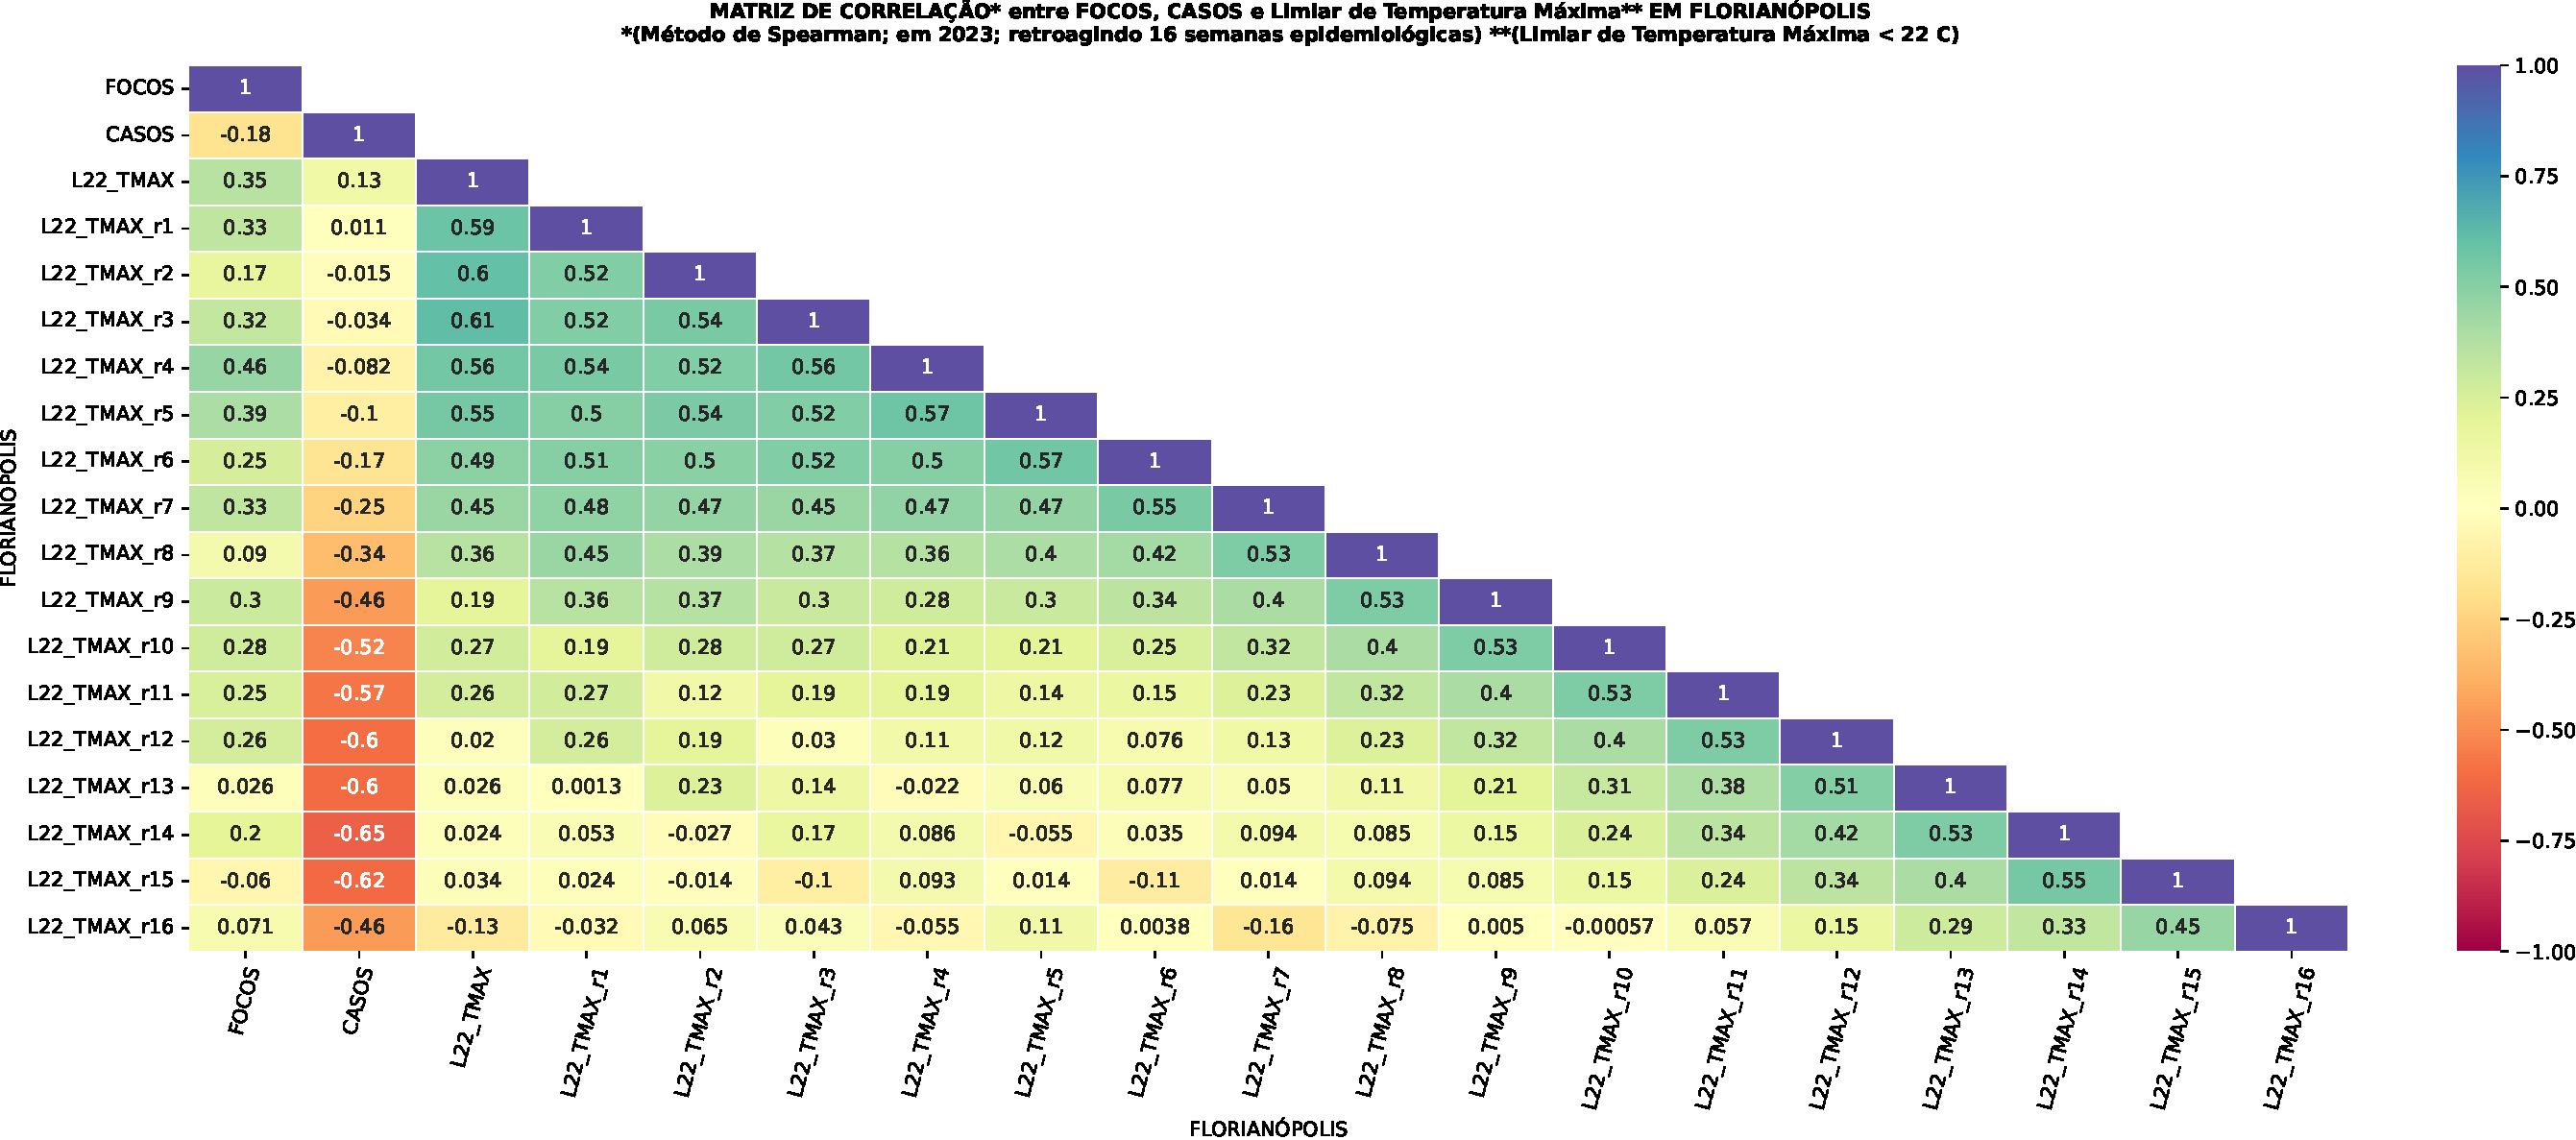
\includegraphics[width=0.47\textwidth]{figuras/matriz_correlacao_spearman_tmax_FLORIANOPOLIS_r16s_2023_LIMIAR22.pdf}
        }
    \subfloat[Limiar - 30 C \label{fig: corr_LIMtmax_FLO30lim}]{
        \centering
        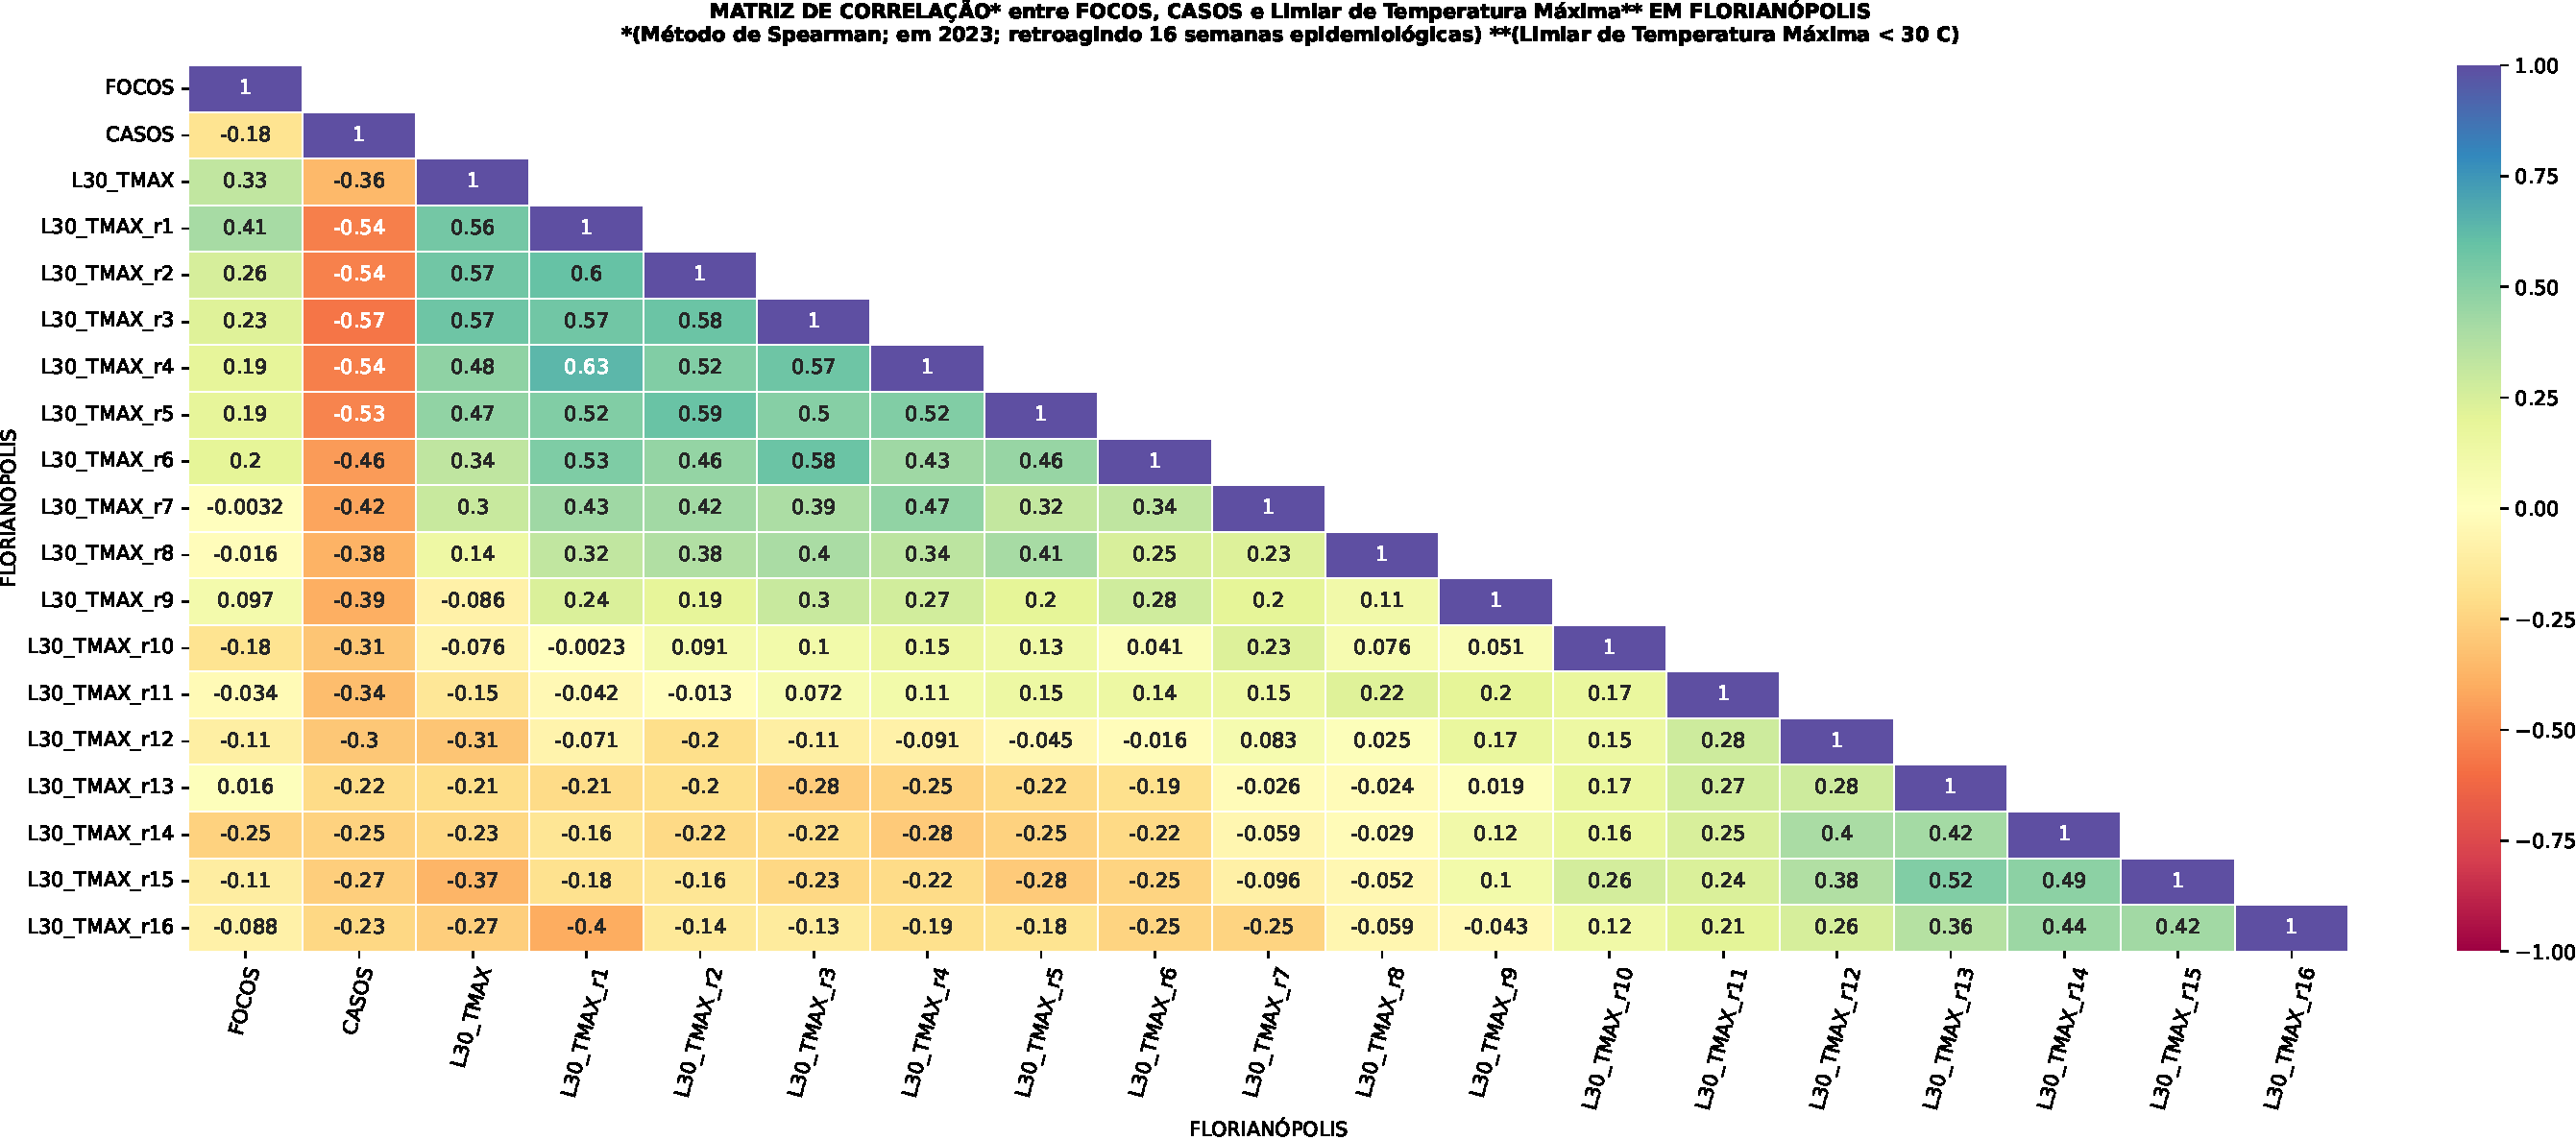
\includegraphics[width=0.47\textwidth]{figuras/matriz_correlacao_spearman_tmax_FLORIANOPOLIS_r16s_2023_LIMIAR30.pdf}
        }
        \hfill
    \end{center}
    \small{Fonte: Elaboração própria (2024).}
\end{figure}

Na sequência, analisar-se-á correlações dos limiares climatológicos obtidos no município de Itajaí (figura \ref{fig: matriz_corr_LIM_ITAretro}). Pode-se verificar correlação baixa positiva entre focos de \latim{Aedes} sp. e temperatura mínima acima do limiar de 16 C, reduzindo intensidade após limiar de 20 C, quando retrocedido três (3) semanas epidemiológicas (figura \ref{fig: corr_LIM_ITAretro3s}). A maior correlação entre focos e temperatura máxima ocorreu abaixo do limiar de 30 C, ainda assim como correlação baixa positiva. Sobre a precipitação, retrocedendo três (3) semanas apidemiológicas, obteve correlação baixa positiva entre focos de \latim{Aedes} sp. nos limiares acima de 35 mm.
É interessante observar que esses mesmo limiares apresentaram correlação baixa positiva, tendendo a média, entre o limiar de temperatura máxima de 32 C. Além de que o limiar de precipitação acima de cinco (5) mm apresentou correlação média positiva entre a temperatura mínima acima de 18 C. Em relação aos casos de dengue, nessas três (3) semanas retrocedidas, as maiores correlações, altas e negativas, ocorreram com os limiares de temperatura mínima acima de 16 C. \textcolor{red}{Discutir tudo isso.} A quinta (5ª) semana epidemiológica retrocedida também é digna de nota em Itajaí (figura \ref{fig: corr_LIM_ITAretro5s}), as correlações entre limiares de temperatura mínima e casos de dengue, nessas cinco (5) semanas retrocedidas, apresentaram maiores valores, altas e negativas, e ocorreram com os limiares de 16 C, 18 C e 20 C. Em relação aos focos de \latim{Aedes} sp., o maior valor, mesmo que uma correlação baixa positiva, ocorreu entre o limiar de temperatura máxima abaixo de 24C. \textcolor{red}{Discutir.}

\begin{figure}[htbp]
    \begin{center}
    \caption{Matriz de correlações entre focos de \latim{Aedes} sp., casos de dengue e limiares de variáveis climatológicas em Itajaí, durante o ano de 2023 retrocedendo semanas epidemiológicas, método de Spearman.}
    \label{fig: matriz_corr_LIM_ITAretro}
    \subfloat[Três semanas epidemiológicas \label{fig: corr_LIM_ITAretro3s}]{
        \centering
        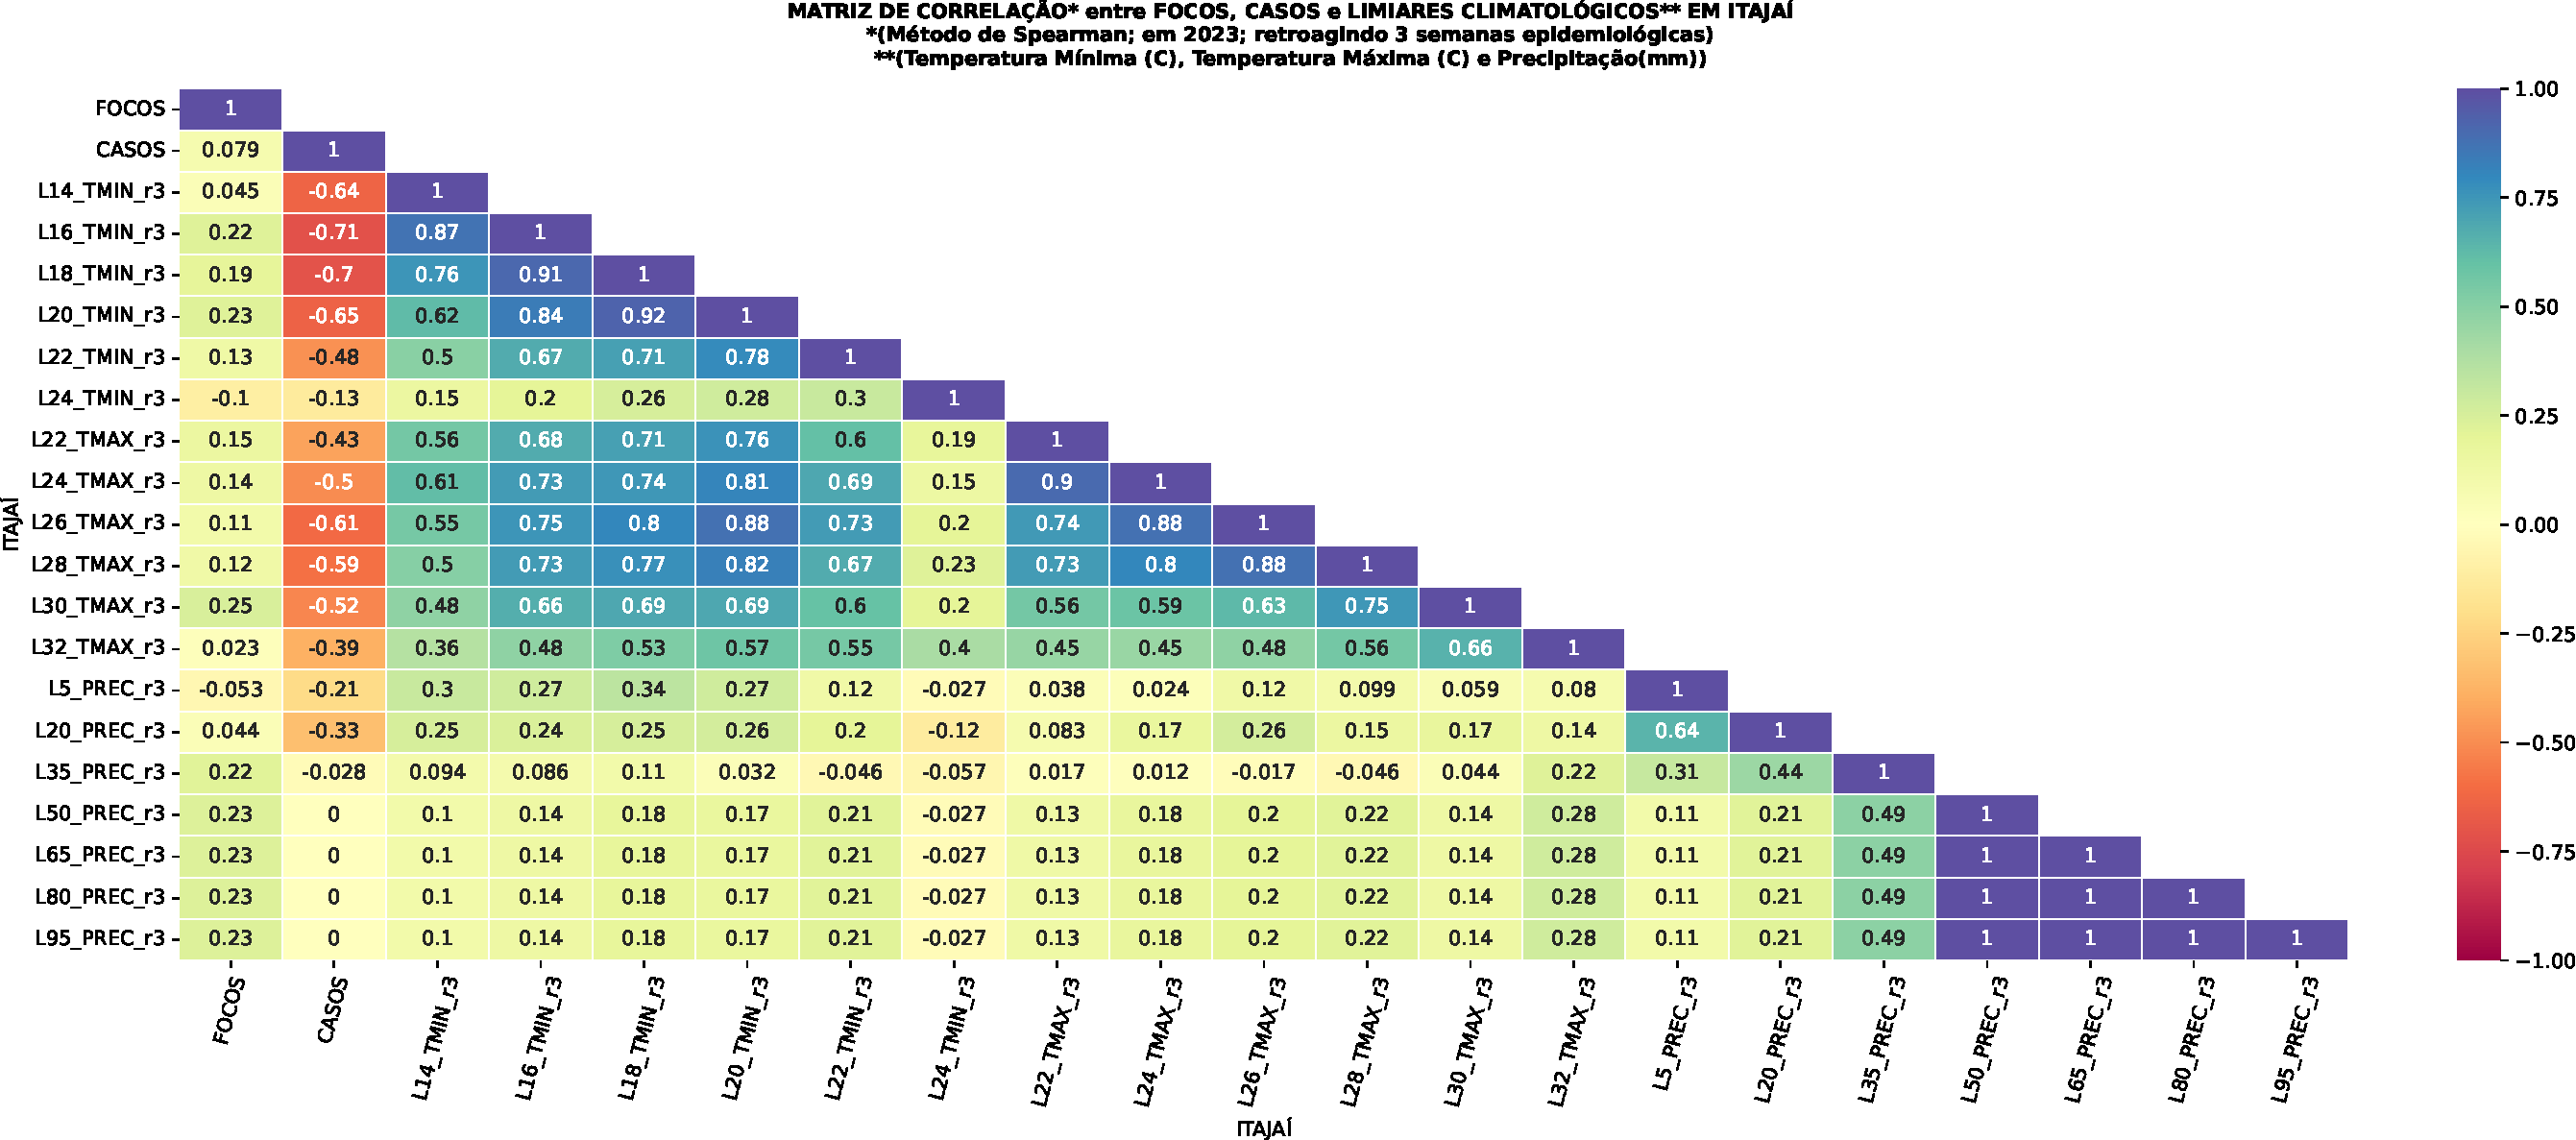
\includegraphics[width=0.47\textwidth]{figuras/matriz_correlacao_spearman_retrolimiar_ITAJAI_2023_r3s.pdf}
        }
    \subfloat[Cinco semanas epidemiológicas \label{fig: corr_LIM_ITAretro5s}]{
        \centering
        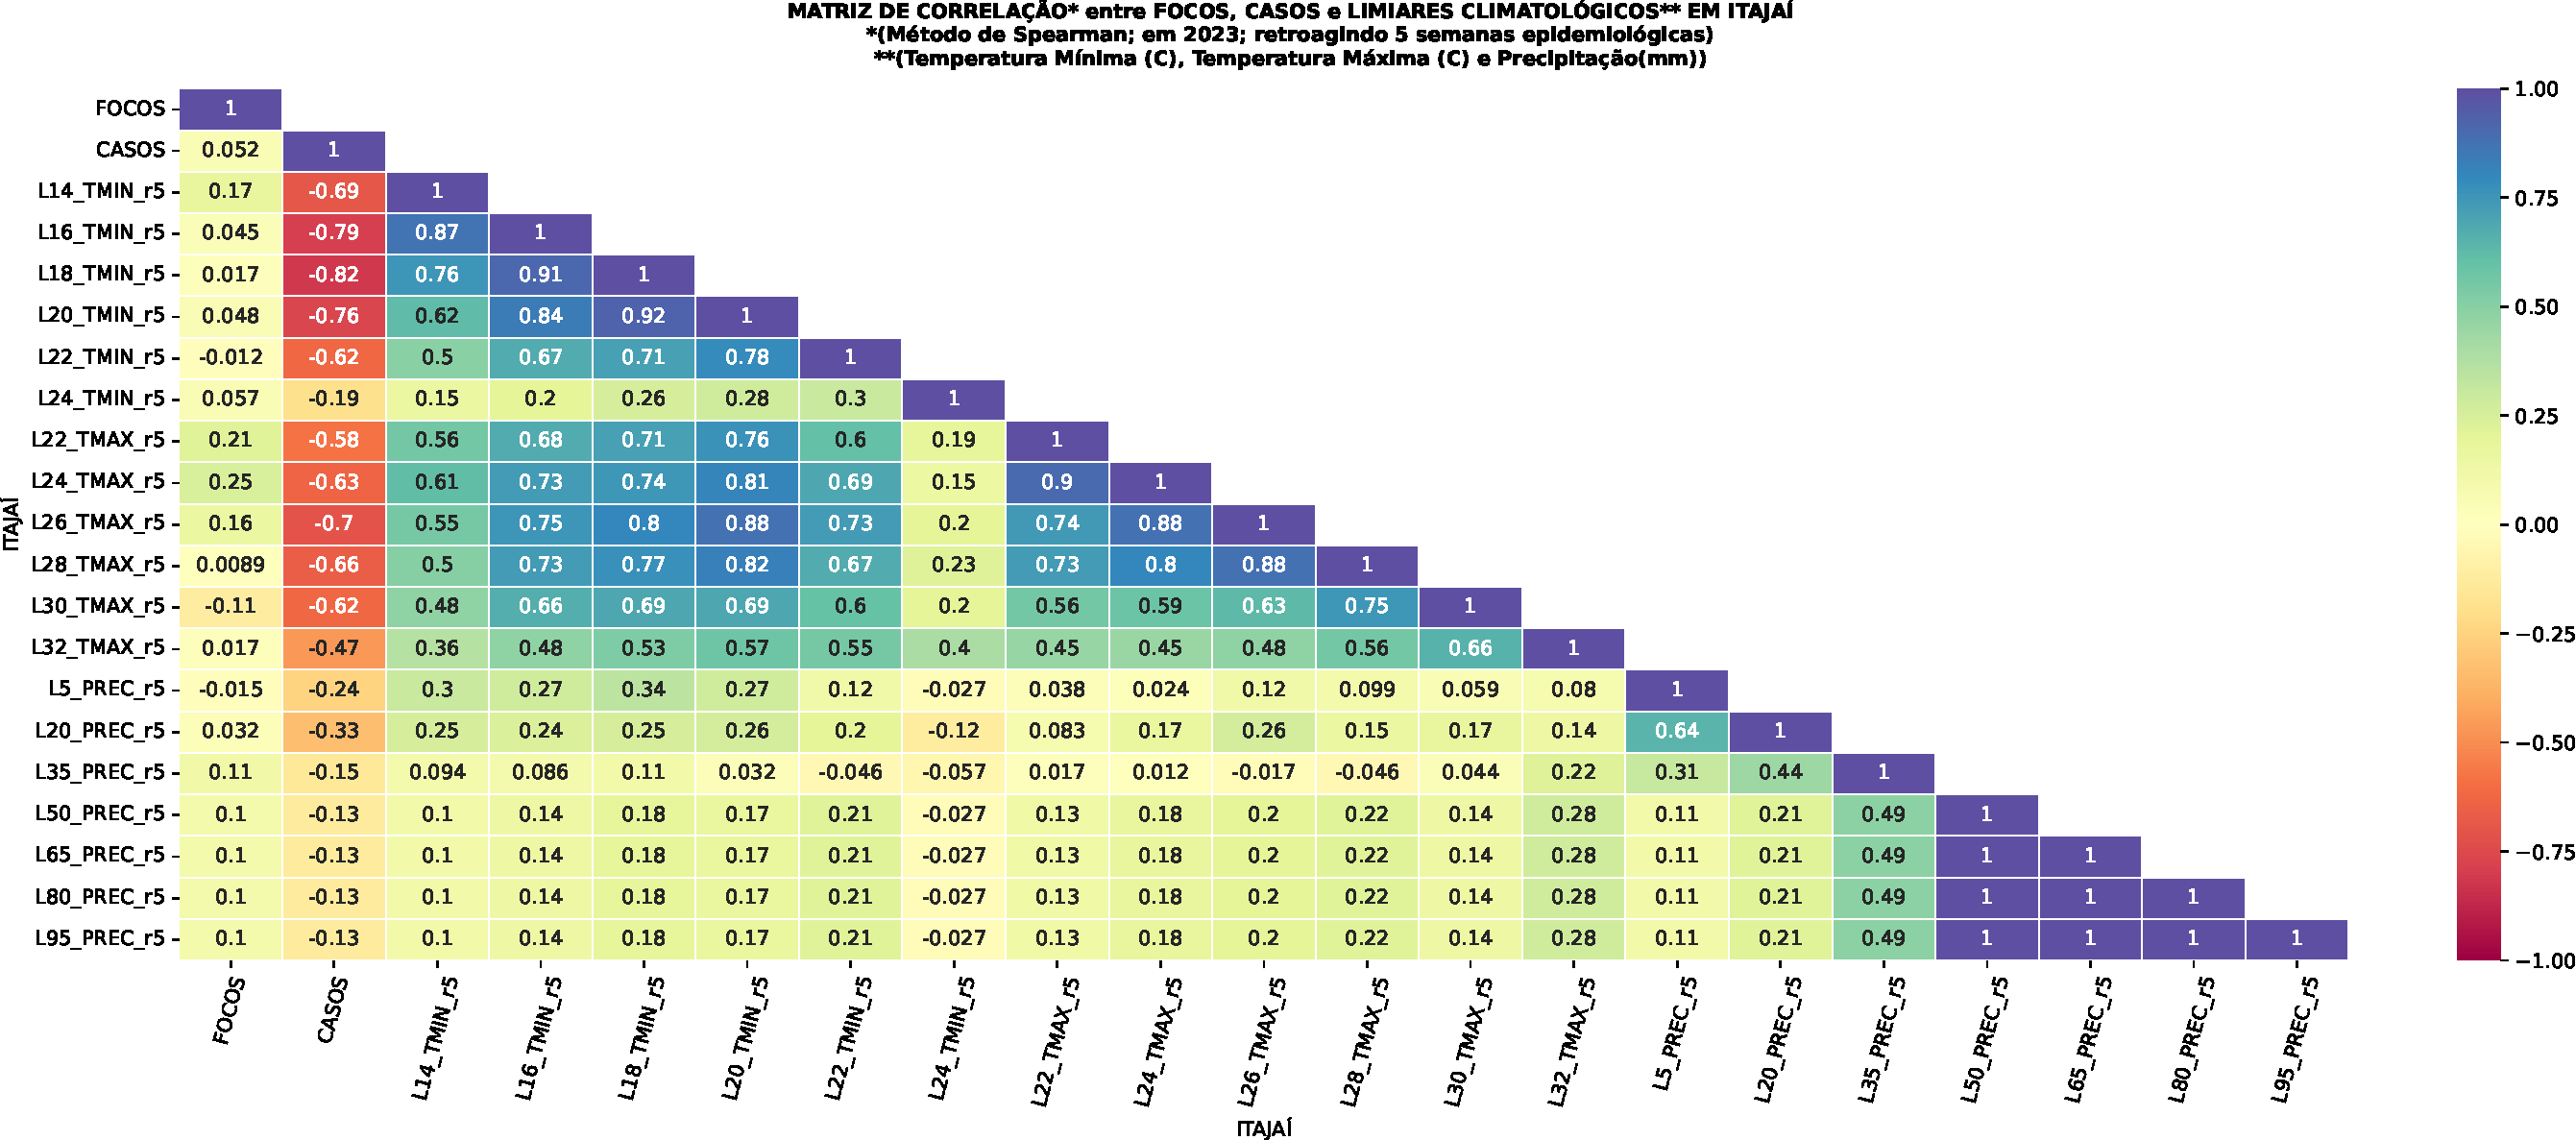
\includegraphics[width=0.47\textwidth]{figuras/matriz_correlacao_spearman_retrolimiar_ITAJAI_2023_r5s.pdf}
        }
        \hfill
    \end{center}
    \small{Fonte: Elaboração própria (2024).}
\end{figure}

\indent Também se analisará os limiares de precipitação em Itajaí de forma mais detalhada (figura \ref{fig: matriz_corr_LIMprec_ITA}). Em relação a focos de \latim{Aedes} sp., observa-se correlação média positiva, quando precipita acima do limiar de dez (10) mm ao retroceder duas (2) semanas epidemiológicas (figura \ref{fig: corr_LIMprec_ITA10lim}) e, também, quando precipita acima de 35 mm ao retroceder três (3) semanas epidemiológicas (figura \ref{fig: corr_LIMprec_ITA35lim}). E relação aos casos de dengue, as maiores correlações, médias negativas, ocorreram no limiar de dez (10) mm ao retroceder três (3), quatro (4) e cinco (5) semanas epidemiológicas. É interessante observar que nesses mesmos períodos de recuo, como comentado em análises anteriores (figura \ref{fig: matriz_corr_LIM_ITAretro}), apresentam-se correlações médias positivas entre temperatura mínima acima de 18 C e limiar de precipitação acima de cinco (5) mm. \textcolor{red}{Discutir.}

\begin{figure}[htbp]
    \begin{center}
    \caption{Matriz de correlações entre focos de \latim{Aedes} sp., casos de dengue e limiares de precipitação (mm) em Itajaí, durante o ano de 2023 retrocedendo semanas epidemiológicas, método de Spearman.}
    \label{fig: matriz_corr_LIMprec_ITA}
    \subfloat[Limiar - 10 mm \label{fig: corr_LIMprec_ITA10lim}]{
        \centering
        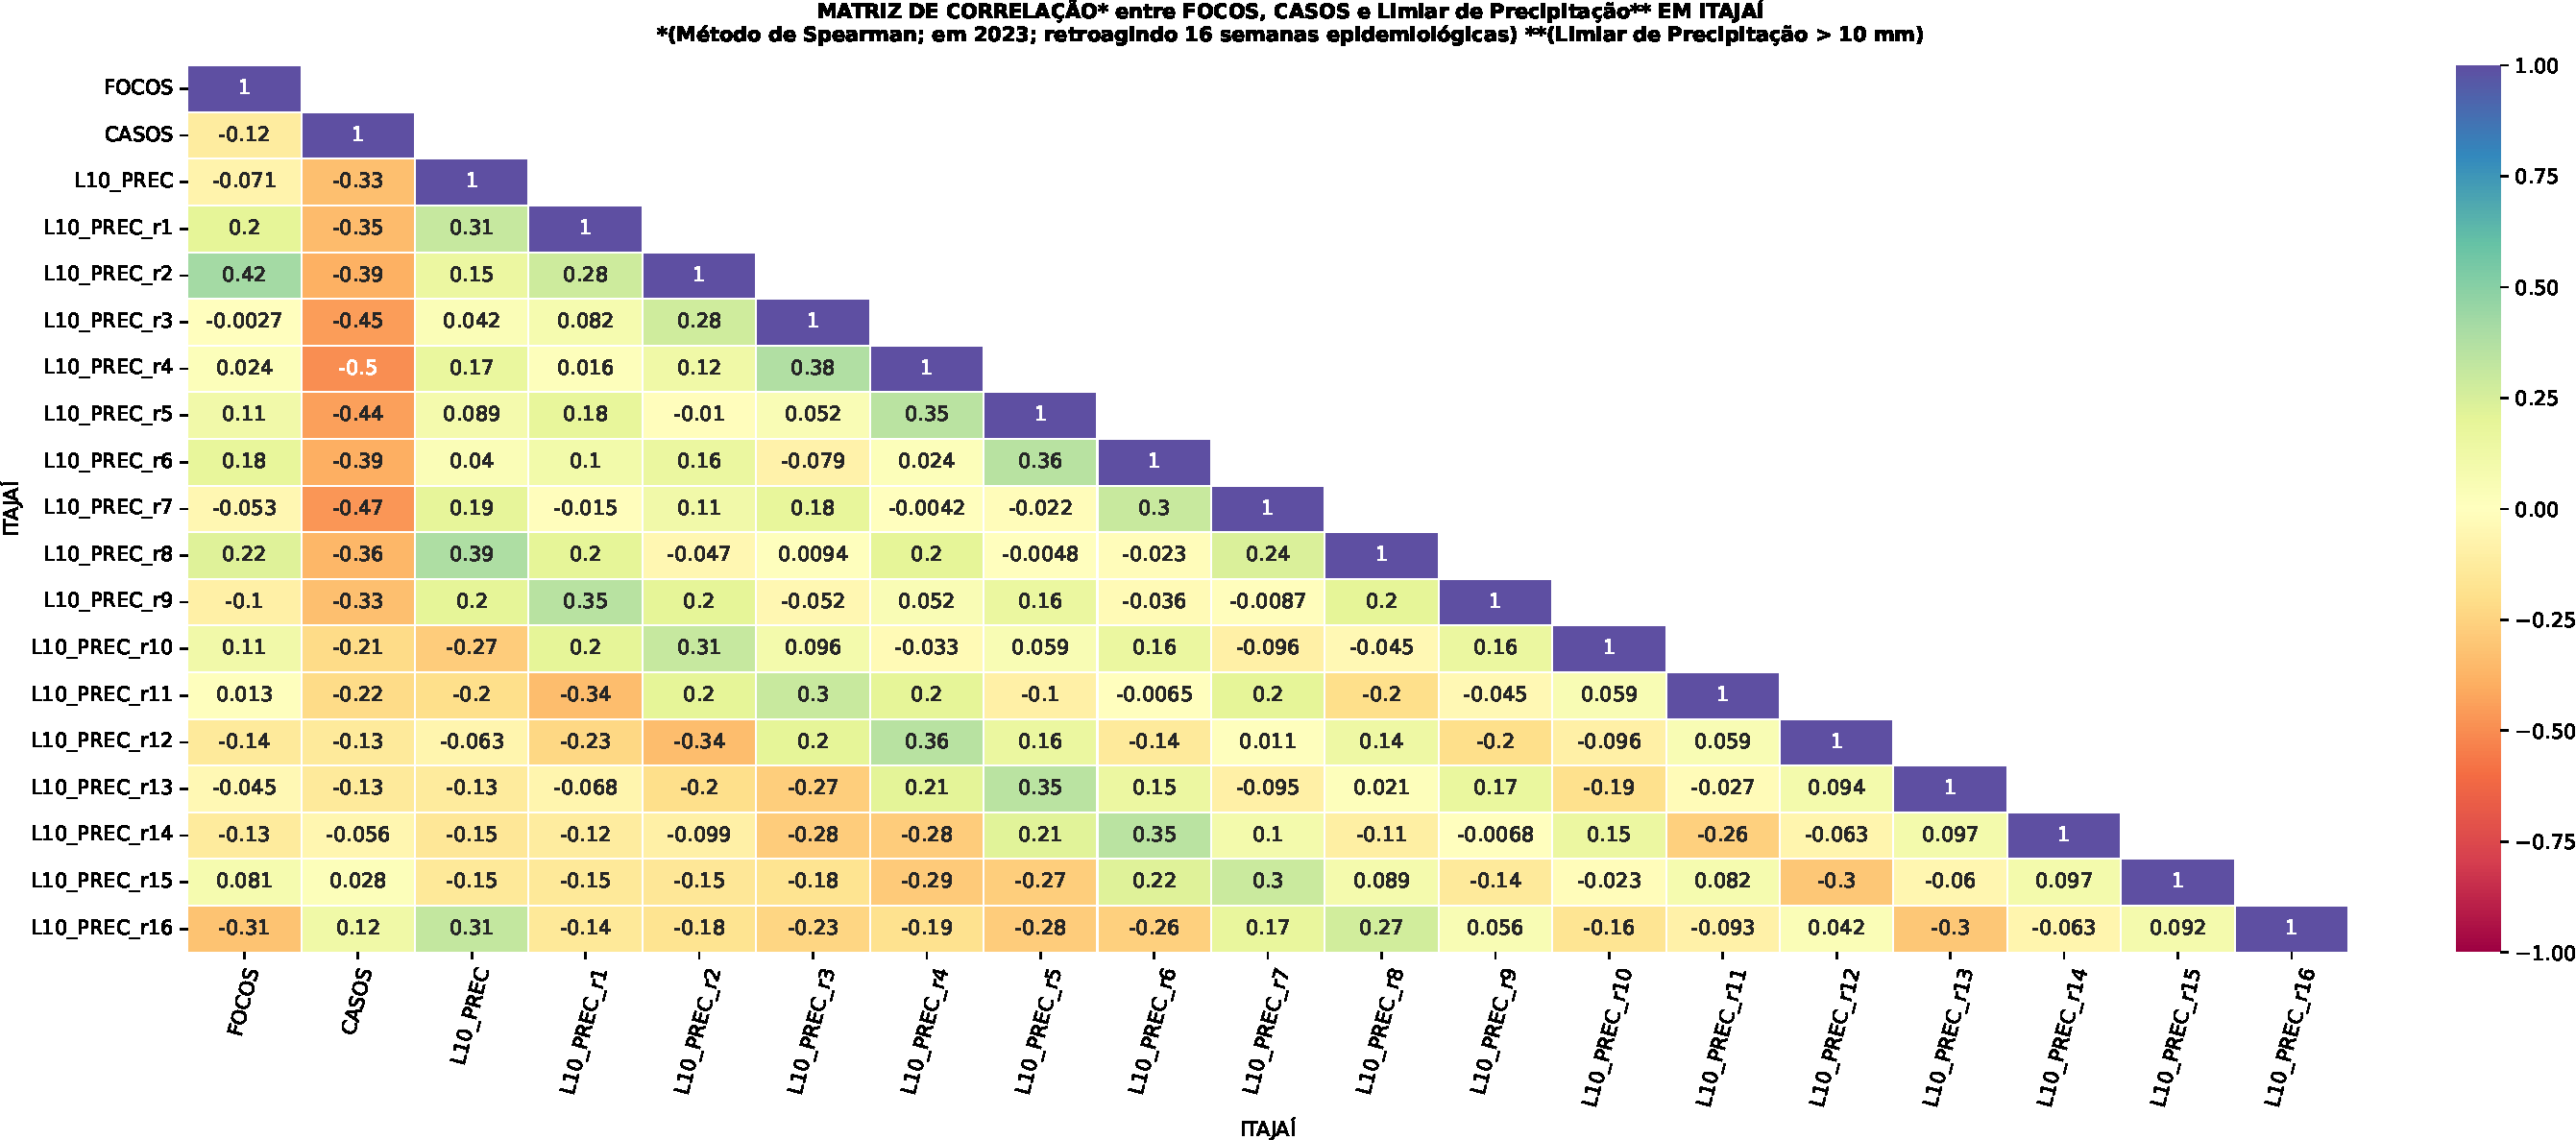
\includegraphics[width=0.47\textwidth]{figuras/matriz_correlacao_spearman_prec_ITAJAI_r16s_2023_LIMIAR10.pdf}
        }
    \subfloat[Limiar - 35 mm \label{fig: corr_LIMprec_ITA35lim}]{
        \centering
        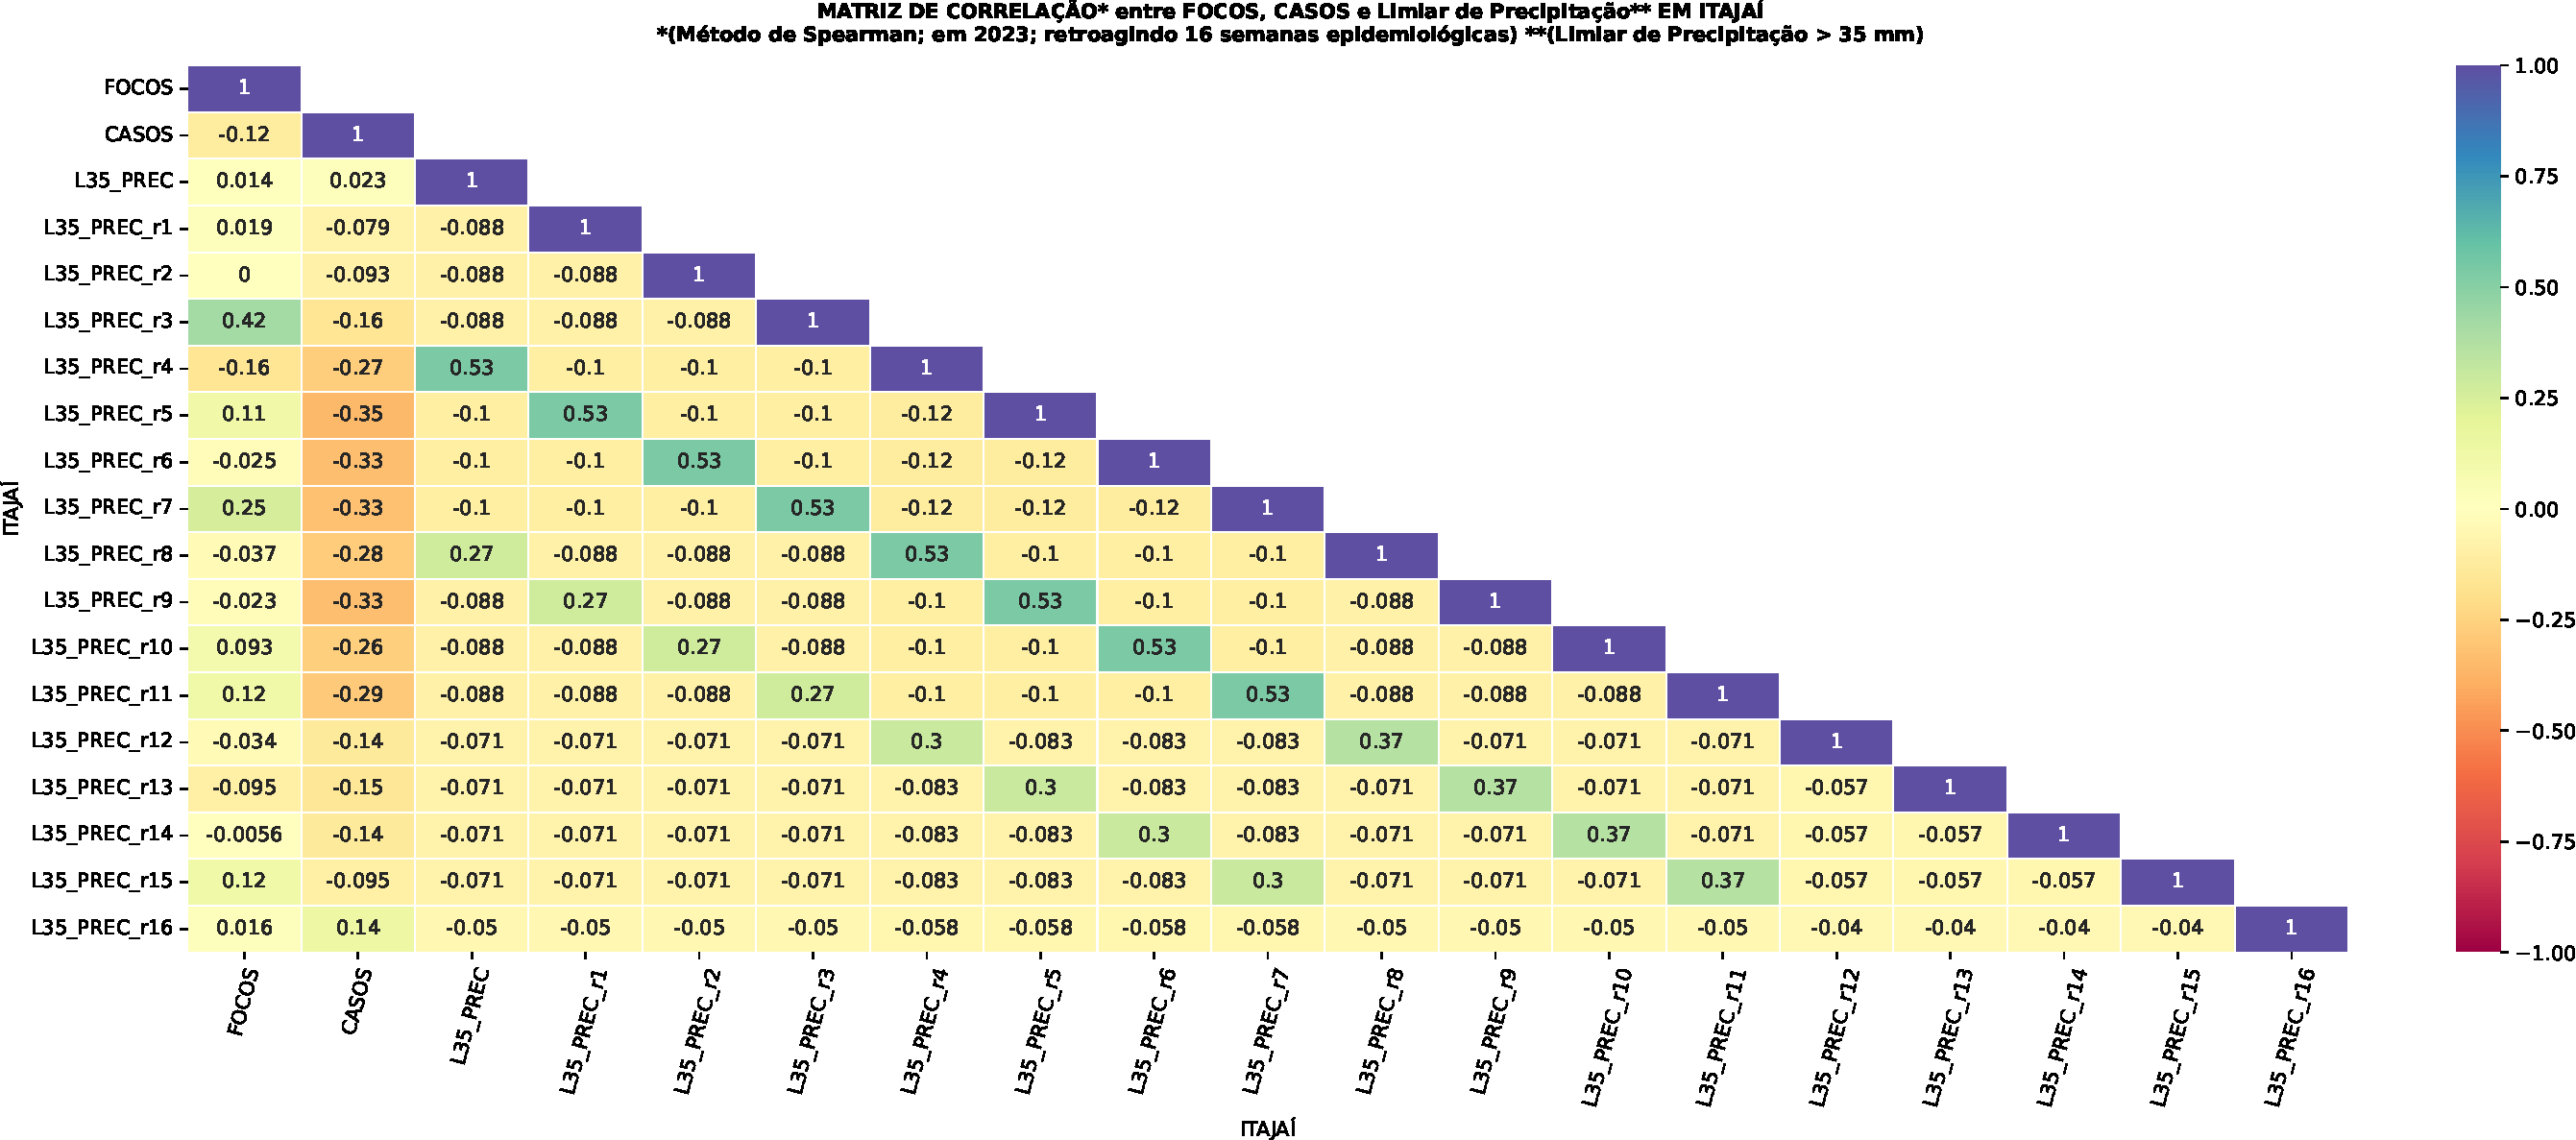
\includegraphics[width=0.47\textwidth]{figuras/matriz_correlacao_spearman_prec_ITAJAI_r16s_2023_LIMIAR35.pdf}
        }
        \hfill
    \end{center}
    \small{Fonte: Elaboração própria (2024).}
\end{figure}

\indent Ademais, ao se analisar as correlações entre temperatura mínima e variáveis entomo-epidemiológicas em Itajaí (figura \ref{fig: matriz_corr_LIMtmin_ITA}), observa-se correlações médias positivas entre os focos de \latim{Aedes} sp. e temperaturas acima do limiar de 14 C (figura \ref{fig: corr_LIMtmin_ITA14lim}) ao recuar uma (1) e cinco (5) semanas epidemiológicas, entre esses períodos as correlações perdem intensidade. Em se tratando de casos de dengue, ganham intensidade nas correlações, médias negativas, quando retroagidos até certo tempo e perdem intensidade ao prosseguir a retroação. \textcolor{red}{Discutir. Semelhança com Floripa.} Em relação ao limiar de 20 C na temperatura mínima (figura \ref{fig: corr_LIMtmin_ITA20lim}), observa-se correlação média positiva entre focos de \latim{Aedes} sp. ao recuar três (3) semanas epidemiológicas. Temperaturas acima desse mesmo limiar, 20 C, correlacionadas entre os casos dengue ganham intensidade nas correlações, médias e altas negativas, quando retroagidos até certo tempo e perdem intensidade ao prosseguir a retroação. \textcolor{red}{Discutir.}

\begin{figure}[htbp]
    \begin{center}
    \caption{Matriz de correlações entre focos de \latim{Aedes} sp., casos de dengue e limiares de temperatura mínima (C) em Itajaí, durante o ano de 2023 retrocedendo semanas epidemiológicas, método de Spearman.}
    \label{fig: matriz_corr_LIMtmin_ITA}
    \subfloat[Limiar - 14 C \label{fig: corr_LIMtmin_ITA14lim}]{
        \centering
        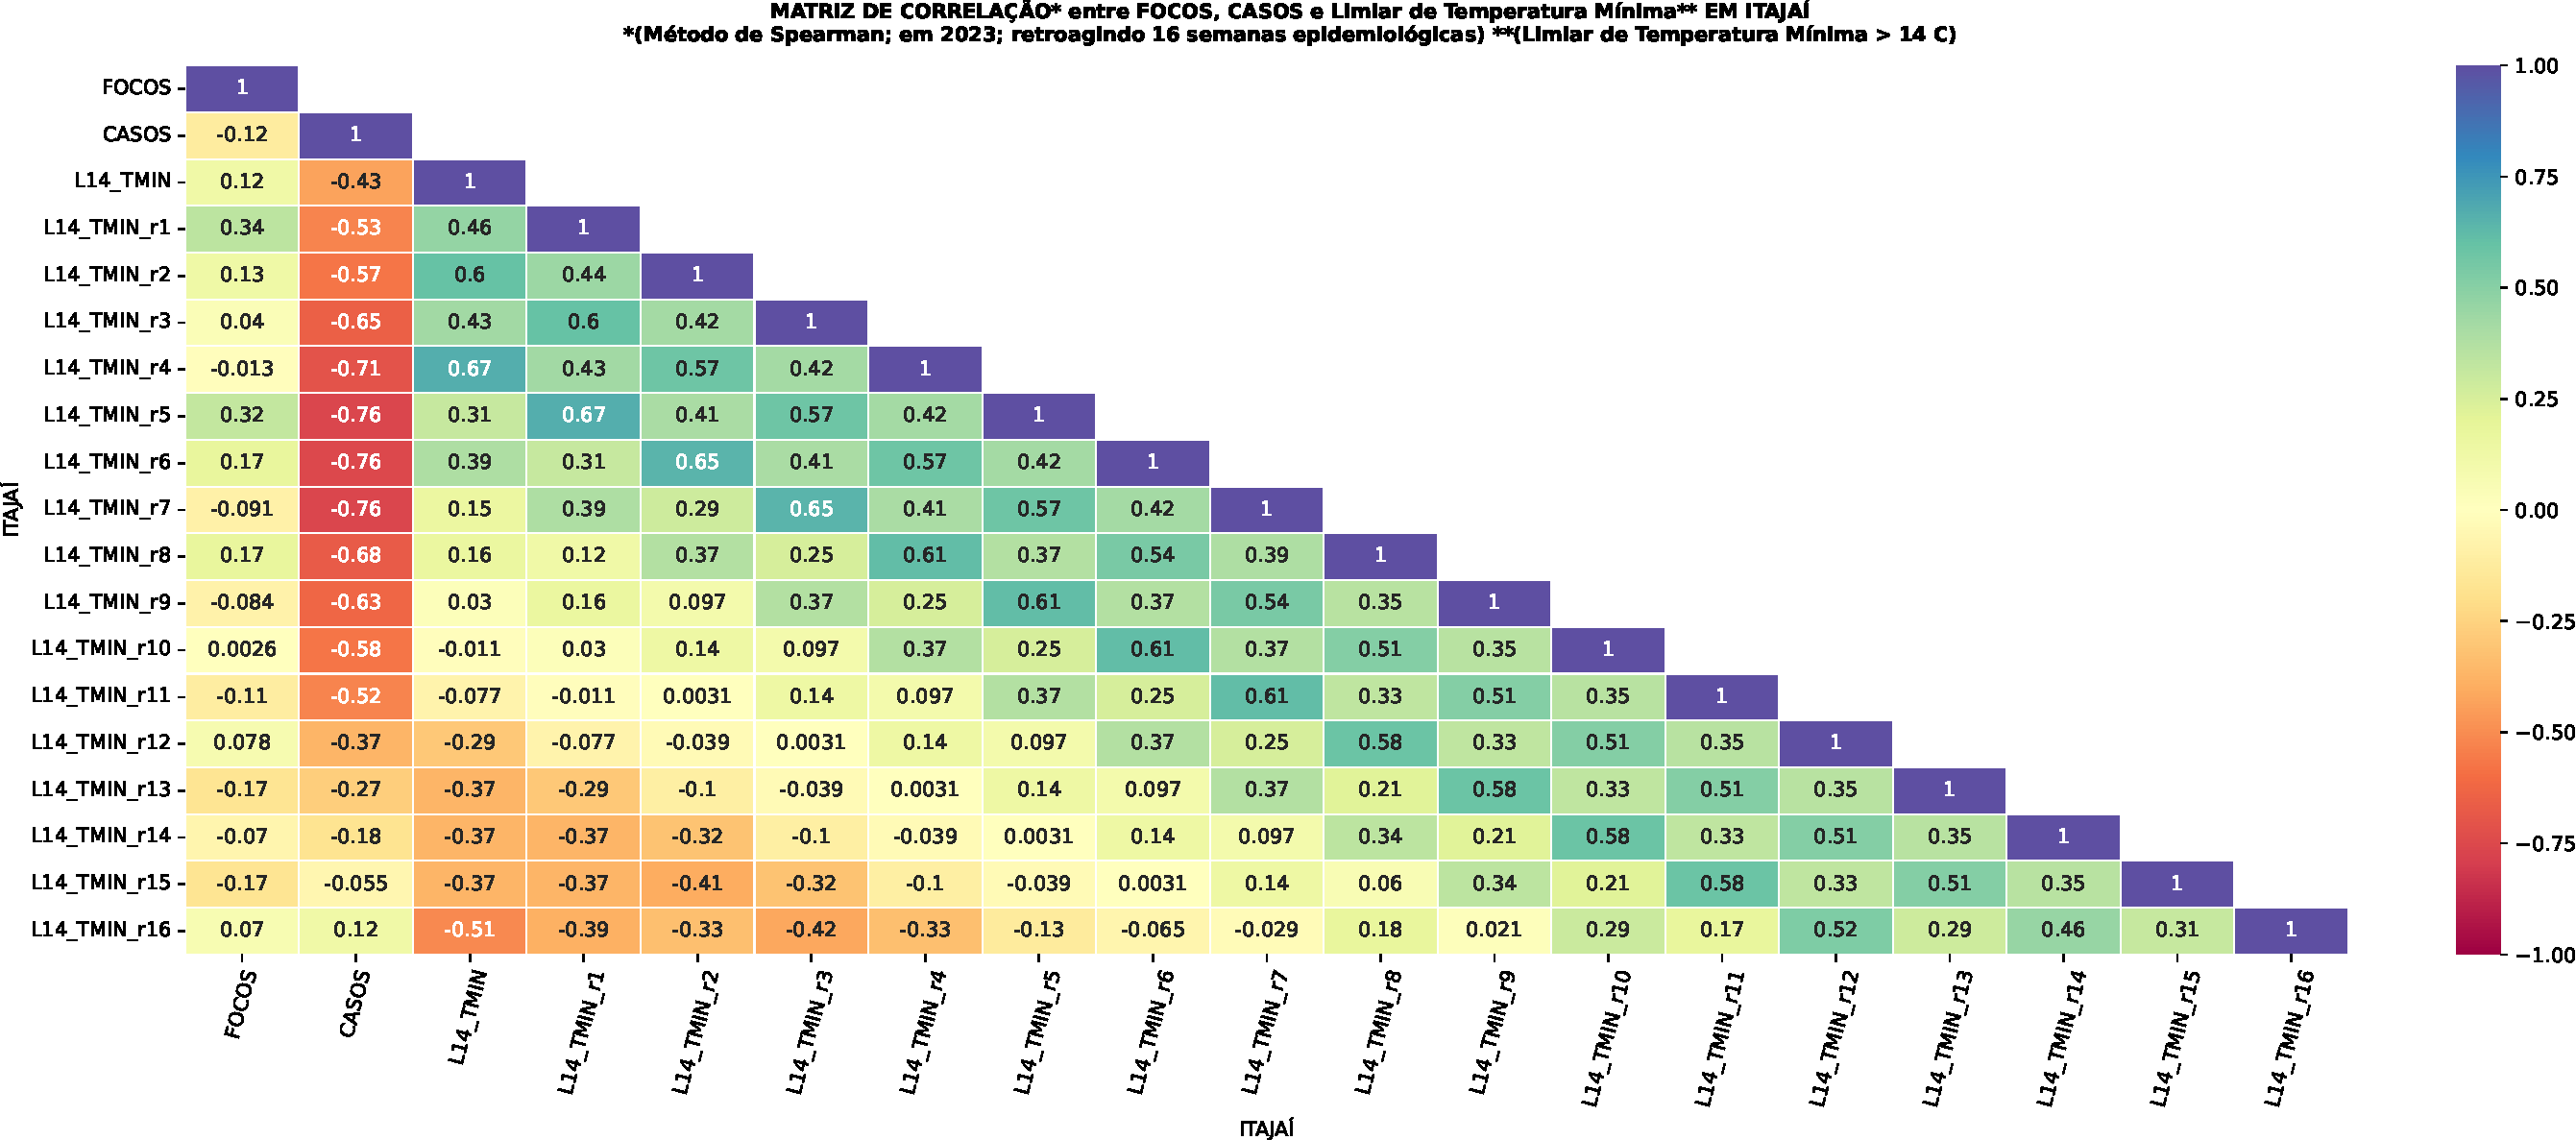
\includegraphics[width=0.47\textwidth]{figuras/matriz_correlacao_spearman_tmin_ITAJAI_r16s_2023_LIMIAR14.pdf}
        }
    \subfloat[Limiar - 20 C \label{fig: corr_LIMtmin_ITA20lim}]{
        \centering
        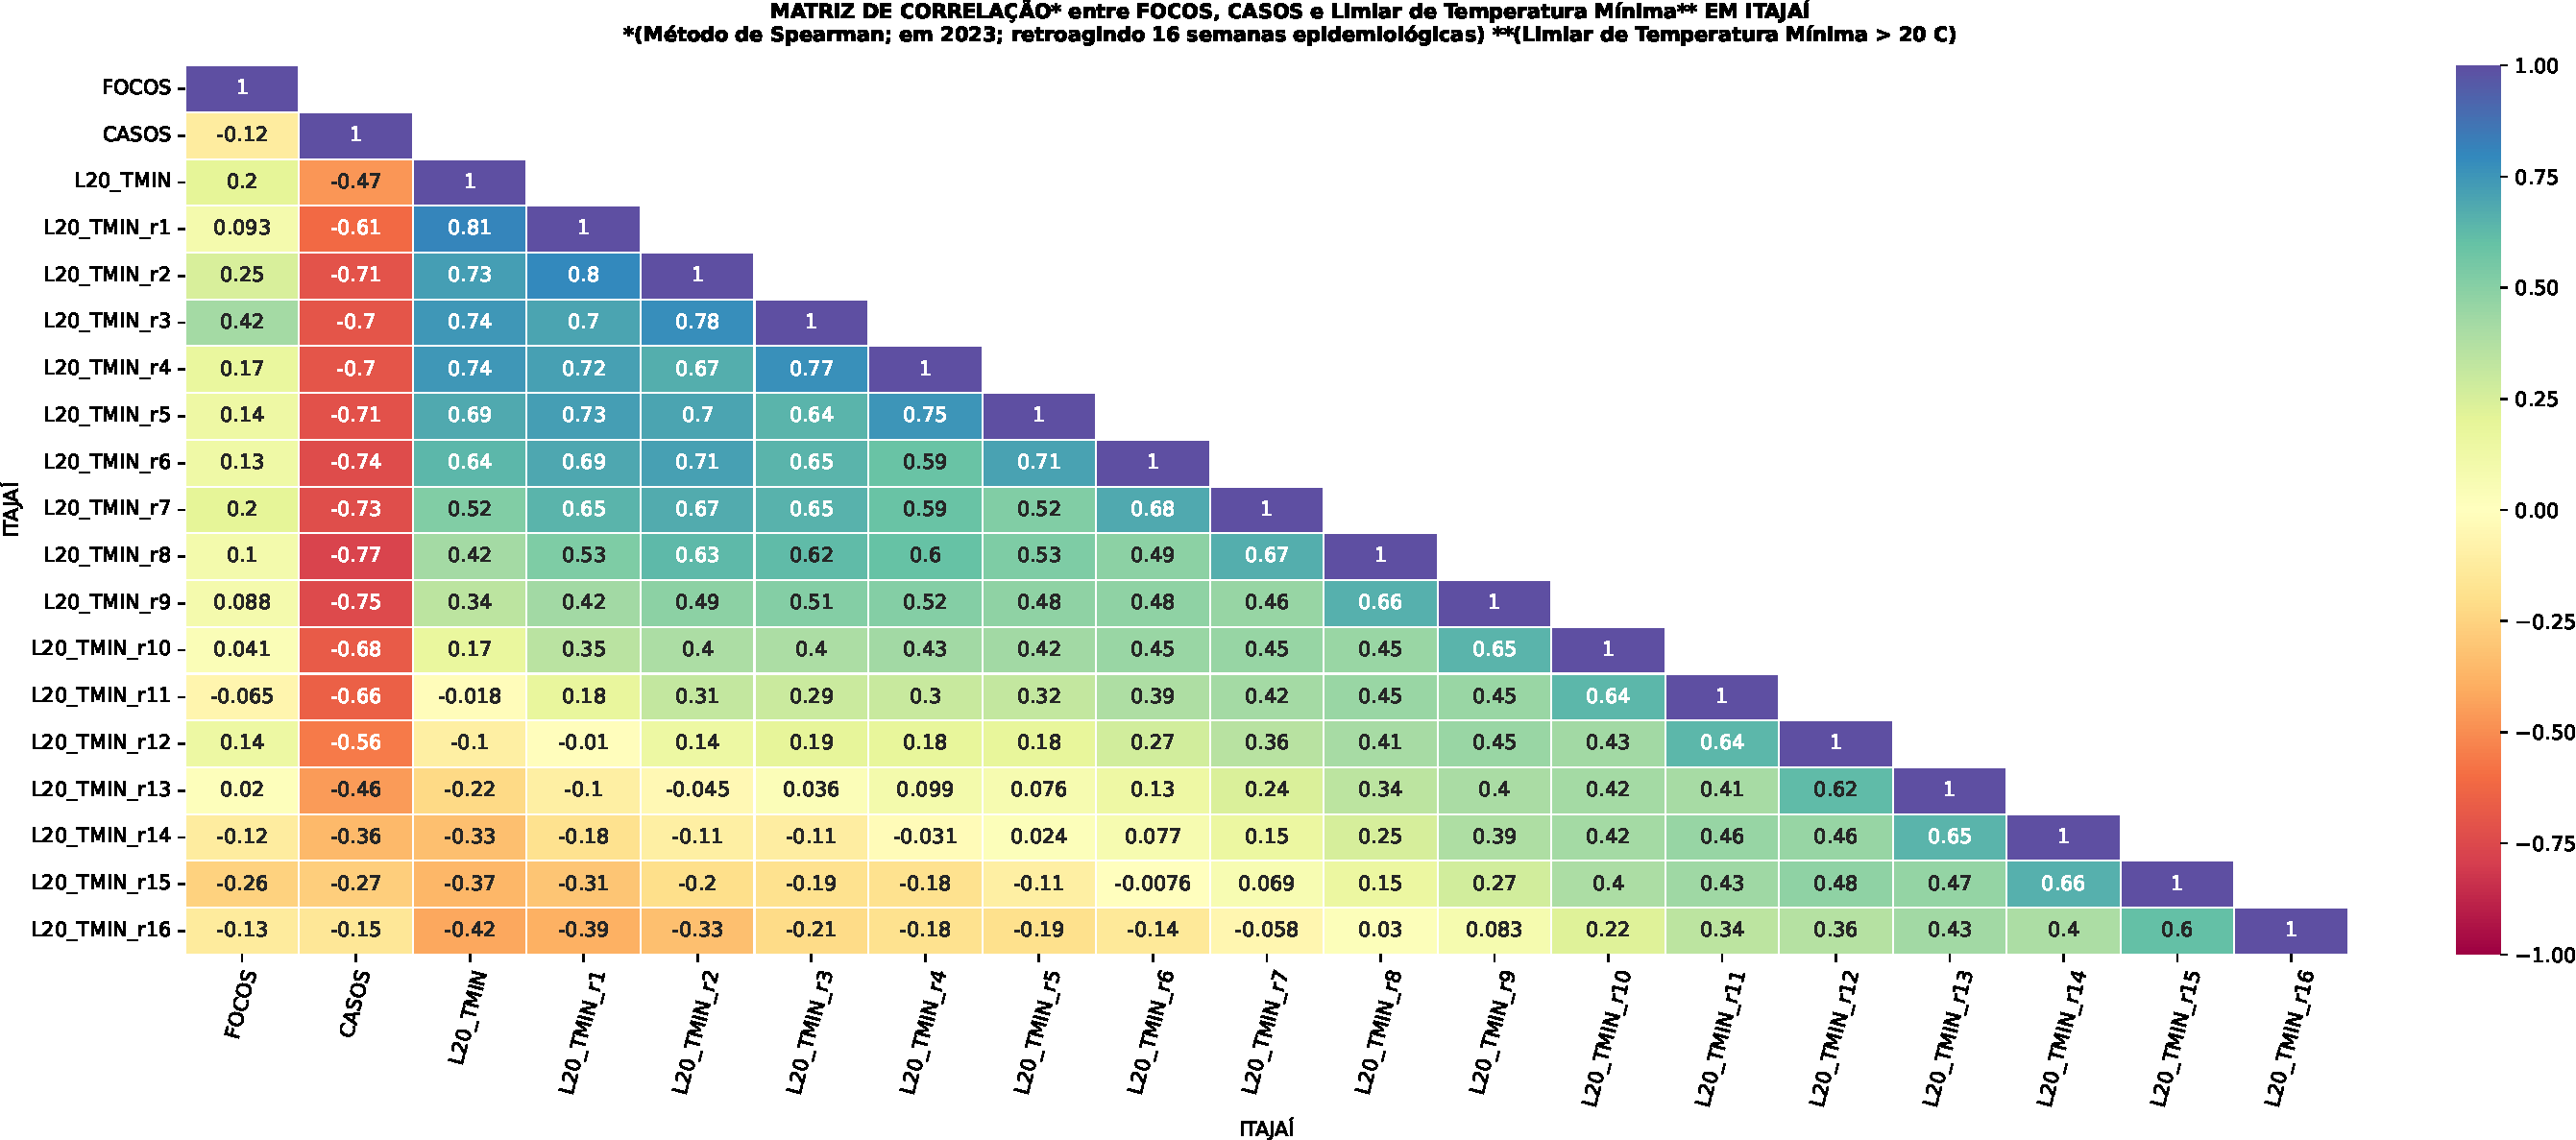
\includegraphics[width=0.47\textwidth]{figuras/matriz_correlacao_spearman_tmin_ITAJAI_r16s_2023_LIMIAR20.pdf}
        }
        \hfill
    \end{center}
    \small{Fonte: Elaboração própria (2024).}
\end{figure}

\indent Ainda, analisando as correlações entre temperatura máxima e variáveis entomo-epidemiológicas em Itajaí (figura \ref{fig: matriz_corr_LIMtmax_ITA}), percebe-se que temperaturas abaixo do limiar de 22 C (figura \ref{fig: corr_LIMtmax_ITA22lim}), tem-se correlações que intensificam entre os casos de dengue, negativamente, quando retroagidos até certo tempo e perdem intensidade ao prosseguir a retroação. Além de que, correlacionando esse mesmo limiar de temperatura máxima, 22 C, e focos de \latim{Aedes} sp., observa-se correlações oscilando entre baixas ou ausentes ao retroceder no tempo. Esses padrões de correlações, observados em focos de \latim{Aedes} sp. e casos de dengue no limiar de 22 C da temperatura máxima, são semelhantes aos observados no limiar de 14 C da temperatura mínima. \textcolor{red}{Discutir.} Sobre o limiar de 30 C da temperatura máxima (figura \ref{fig: corr_LIMtmax_ITA30lim}), correlações entre focos de \latim{Aedes} sp. apresentam intensidade média positiva na própria semana e retrocedendo três (3) semanas epidemiológicas, perdendo intensidade entre esse período e retrocedendo além das três (3) semanas. Correlacionando casos de dengue e esse limiar, 30 C, correlações altas negativas são encontradas ao retroceder pouco no tempo, perdendo intensidade em tempos mais pretéritos. \textcolor{red}{Discutir.}

\begin{figure}[htbp]
    \begin{center}
    \caption{Matriz de correlações entre focos de \latim{Aedes} sp., casos de dengue e limiares de temperatura máxima (C) em Itajaí, durante o ano de 2023 retrocedendo semanas epidemiológicas, método de Spearman.}
    \label{fig: matriz_corr_LIMtmax_ITA}
    \subfloat[Limiar - 22 C \label{fig: corr_LIMtmax_ITA22lim}]{
        \centering
        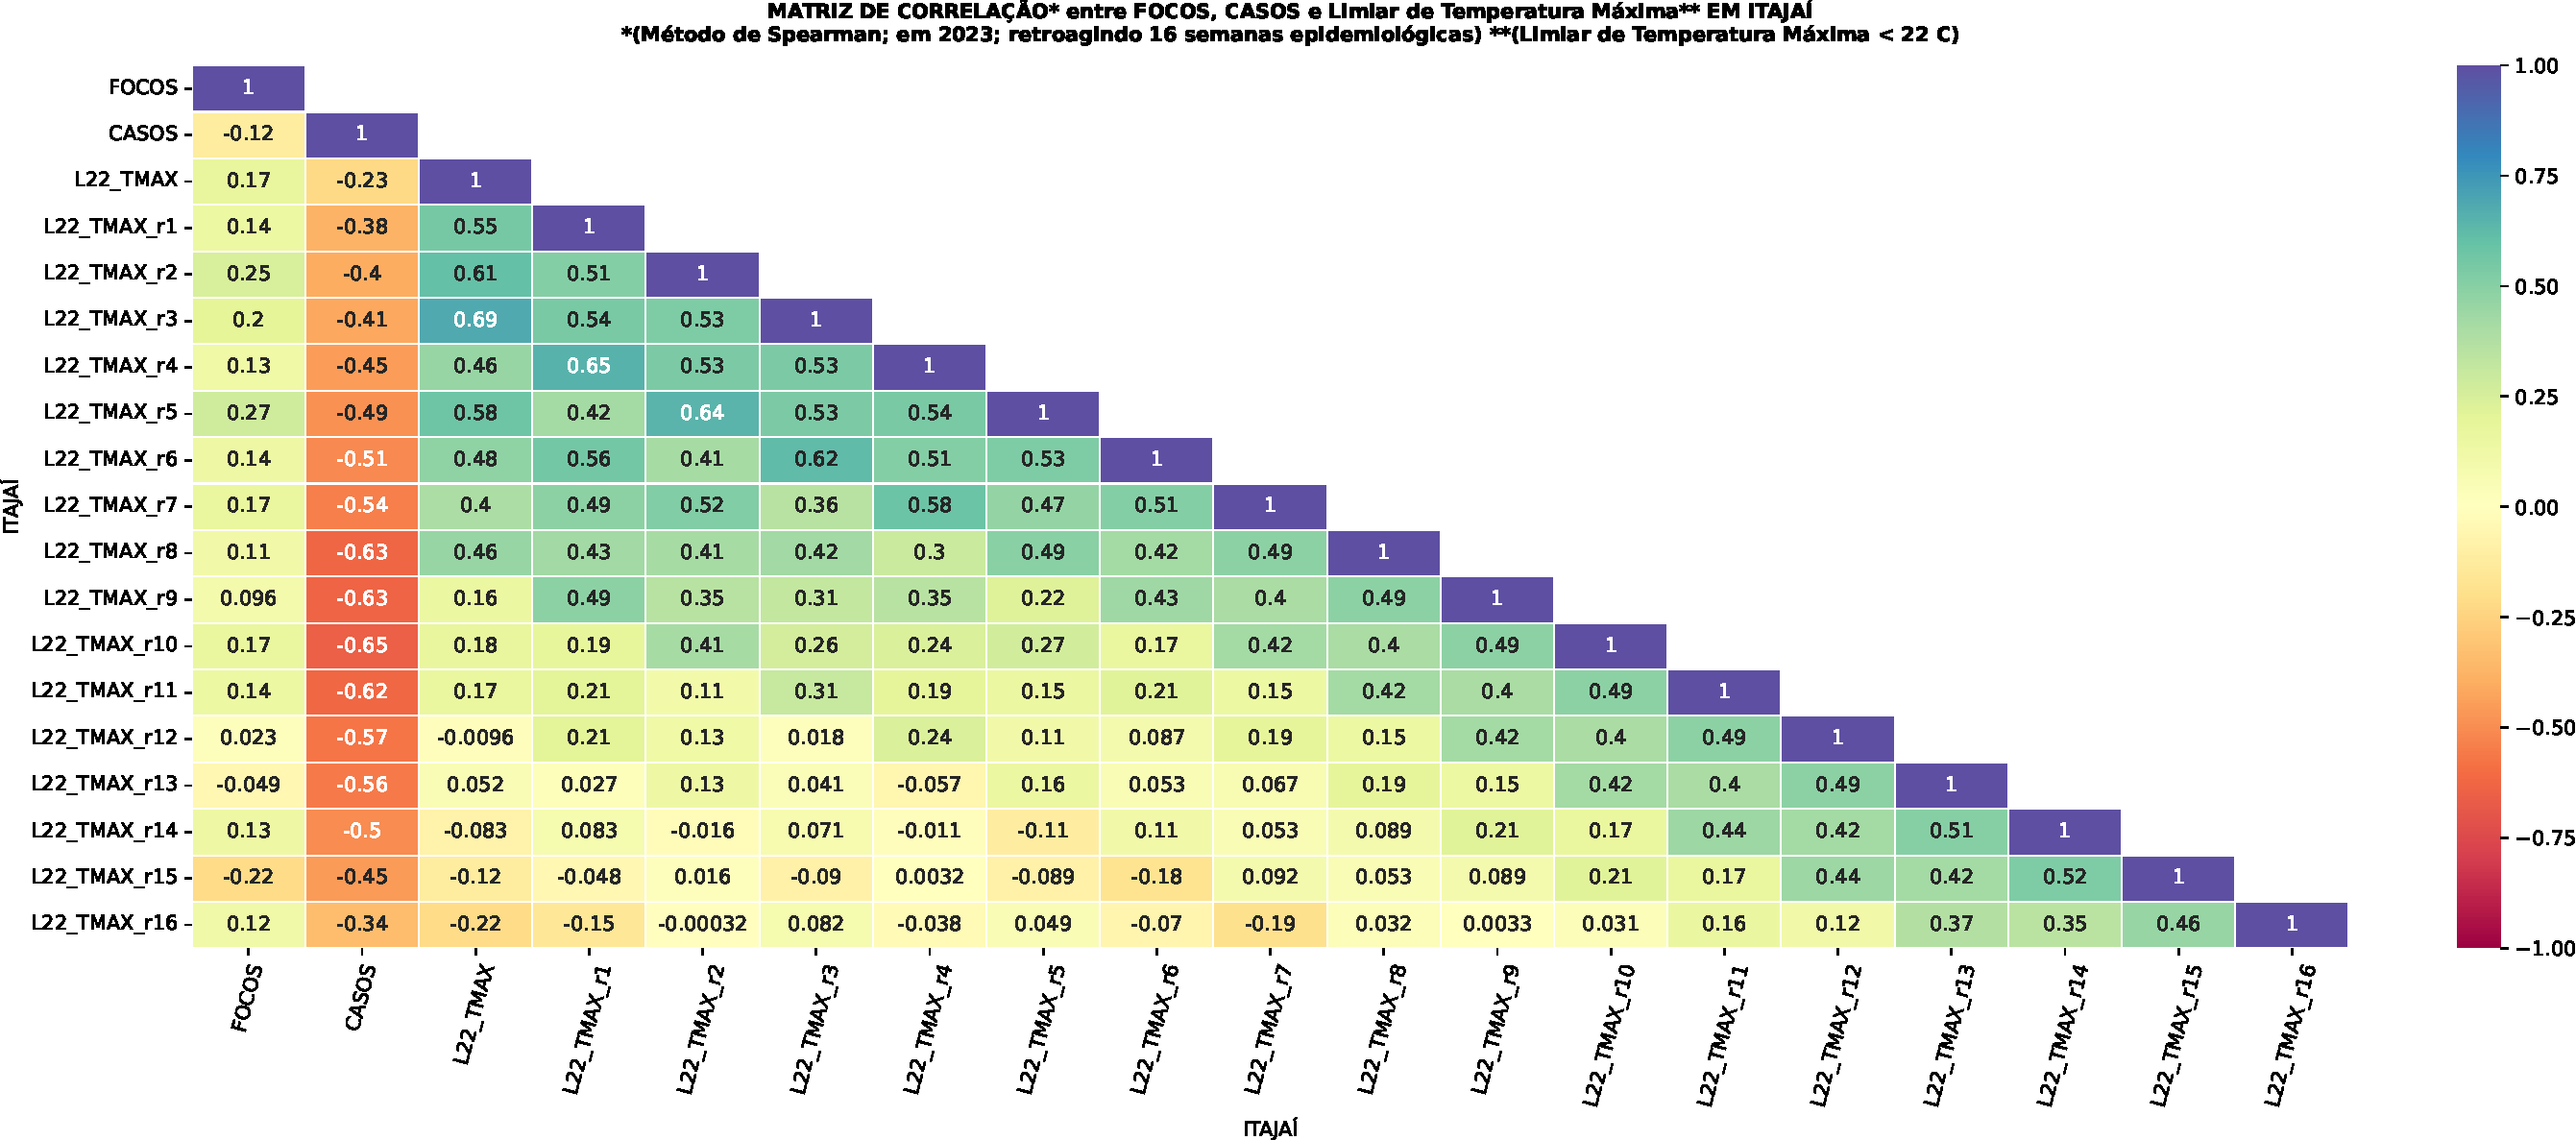
\includegraphics[width=0.47\textwidth]{figuras/matriz_correlacao_spearman_tmax_ITAJAI_r16s_2023_LIMIAR22.pdf}
        }
    \subfloat[Limiar - 30 C \label{fig: corr_LIMtmax_ITA30lim}]{
        \centering
        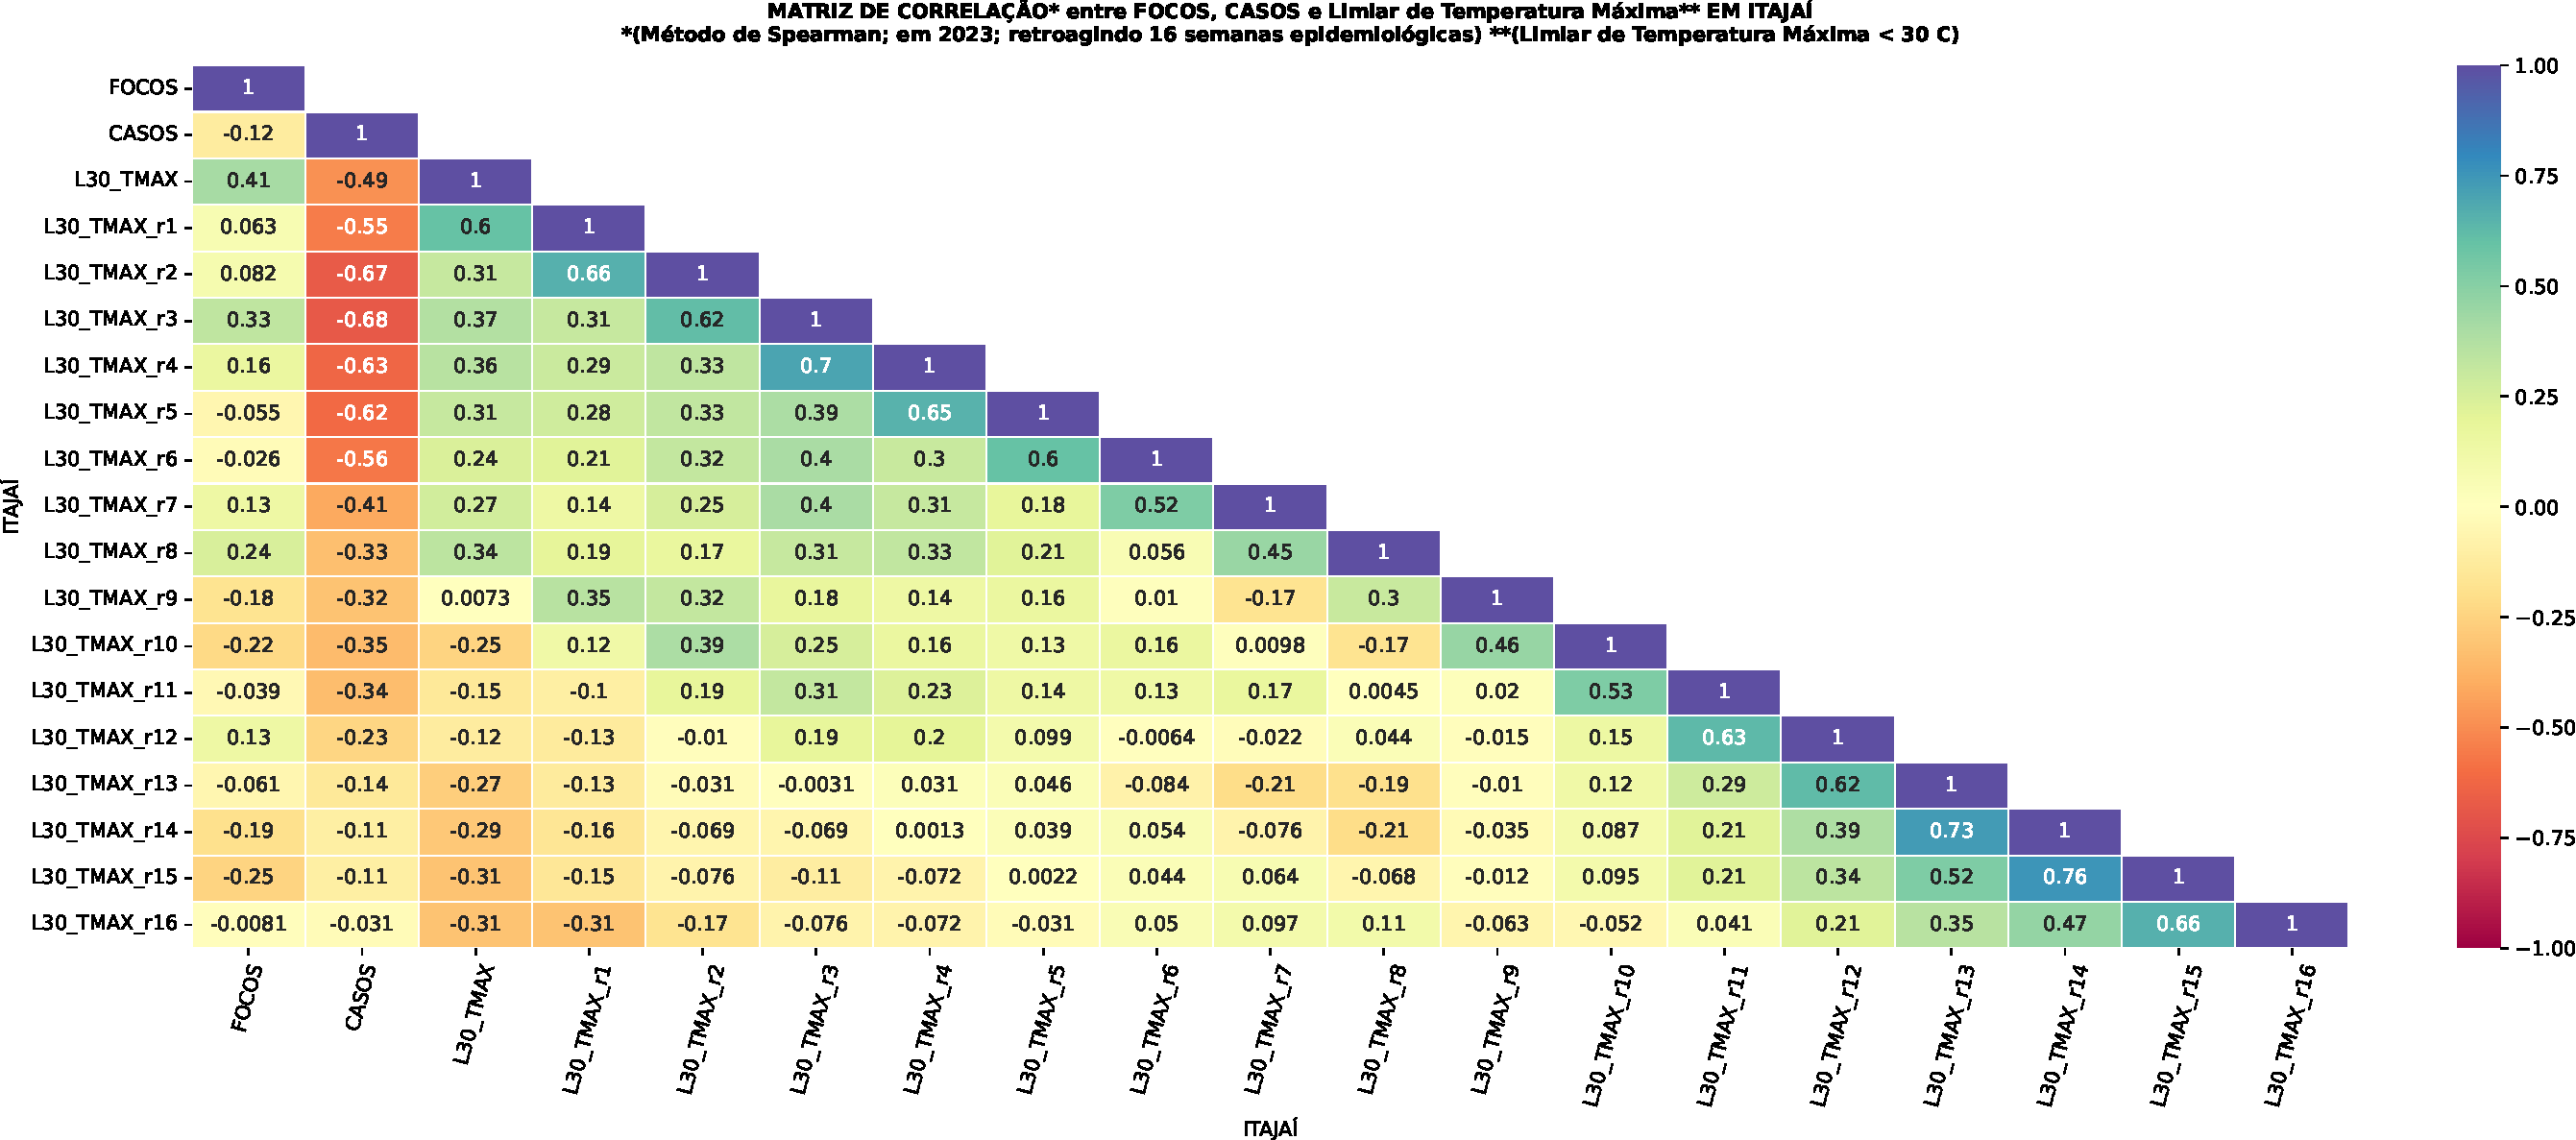
\includegraphics[width=0.47\textwidth]{figuras/matriz_correlacao_spearman_tmax_ITAJAI_r16s_2023_LIMIAR30.pdf}
        }
        \hfill
    \end{center}
    \small{Fonte: Elaboração própria (2024).}
\end{figure}

%%%%%%%%%%%%%%%% JOINVILLE

Passando para o município de Joinville, valores mais expressivos de correlações dos limiares climatológicos foram observados sem retroagir e retrocedendo em três (3) semanas epidemiológicas (figura \ref{fig: matriz_corr_LIM_JOIretro}). Em todas as matrizes de correlações, nessa análise de semanas epidemiológicas retrocedidas, os limiares de precipitação acima de 50 mm não apresentaram valores. Não retrocendendo no tempo e correlacionando com focos de \latim{Aedes} sp. (figura \ref{fig: corr_LIM_JOIretro0s}), tem-se 22 C como o limiar para ambas as temperaturas, mínima e máxima, que apresenta correlações médias positivas. Em relação aos casos de dengue, correlações médias negativas foram observadas nos limiares de 14 C, 16 C e 18 C de temperatura mínima, assim como no limiar de 28 C de temperatura máxima. \textcolor{red}{Discutir.} Ao recuar três (3) semanas epidemiológicas (figura \ref{fig: corr_LIM_JOIretro3s}), tem-se correlação média positiva entre o limiar de 24 C da temperatura mínima e os focos de \latim{Aedes} sp. Sobre os casos de dengue, apresentaram ascenção e declínio da intensidade das correlações, mesmo que negativas, nos limiares de 18 C de temperatura mínima e 28 C de temperatura máxima. Ambos os períodos apresentaram correlações baixas, tanto negativas quanto positivas, entre focos de \latim{Aedes} sp. e precipitação nos três (3) limiares presentes. \textcolor{red}{Discutir.}

\begin{figure}[htbp]
    \begin{center}
    \caption{Matriz de correlações entre focos de \latim{Aedes} sp., casos de dengue e limiares de variáveis climatológicas em Joinville, durante o ano de 2023 sem retroagir e retrocedendo três (3) semanas epidemiológicas, método de Spearman.}
    \label{fig: matriz_corr_LIM_JOIretro}
    \subfloat[Sem retroação \label{fig: corr_LIM_JOIretro0s}]{
        \centering
        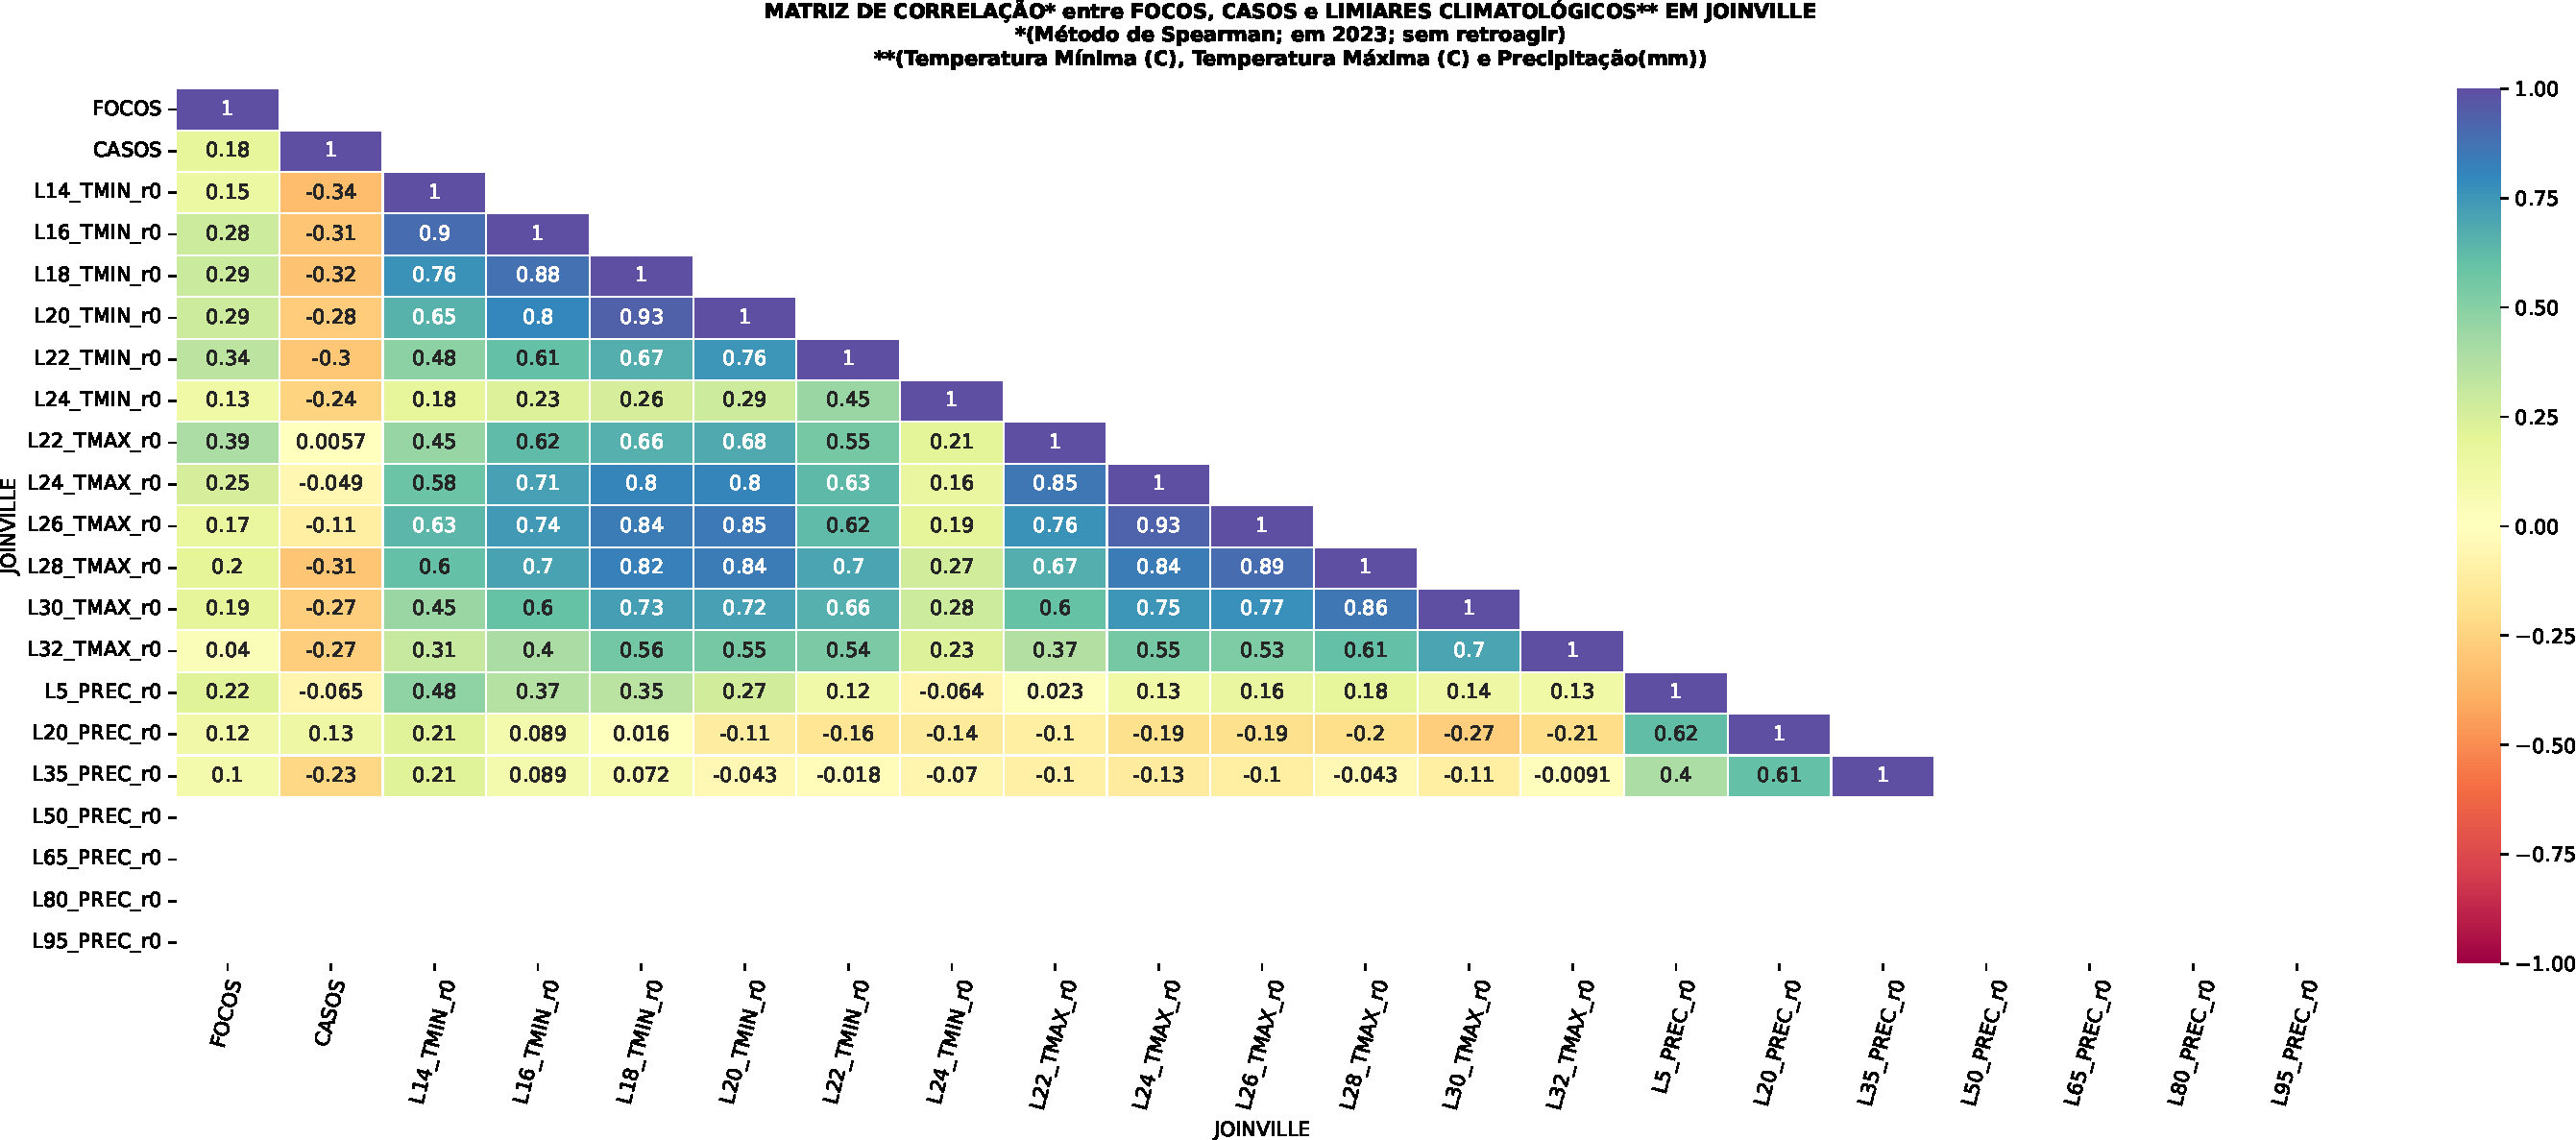
\includegraphics[width=0.47\textwidth]{figuras/matriz_correlacao_spearman_retrolimiar_JOINVILLE_2023_r0s.pdf}
        }
    \subfloat[Três semanas epidemiológicas \label{fig: corr_LIM_JOIretro3s}]{
        \centering
        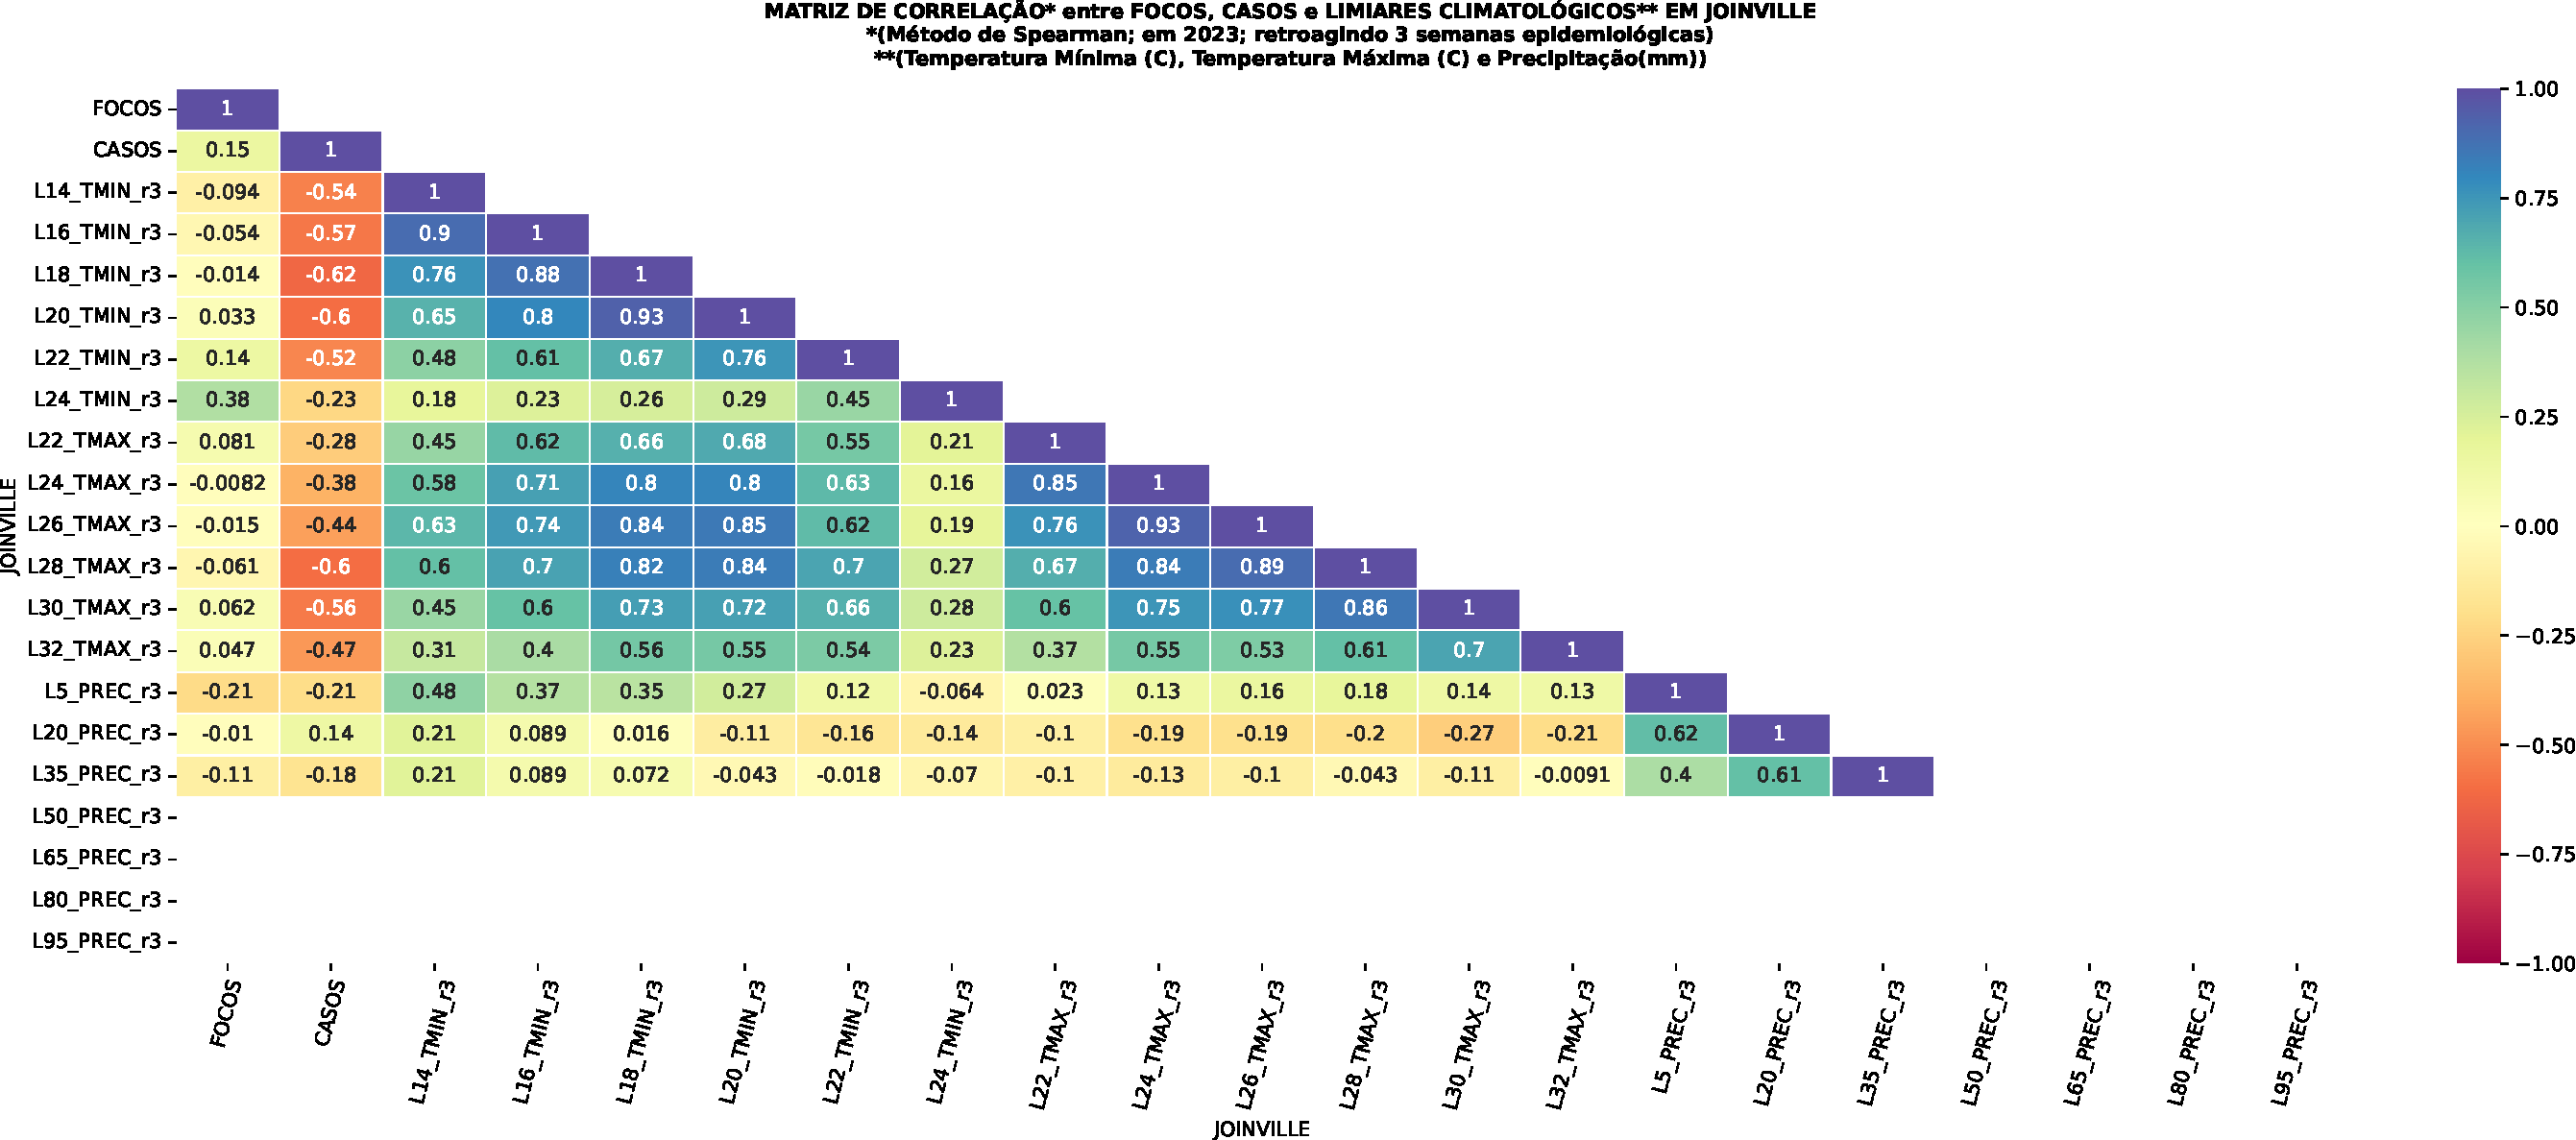
\includegraphics[width=0.47\textwidth]{figuras/matriz_correlacao_spearman_retrolimiar_JOINVILLE_2023_r3s.pdf}
        }
        \hfill
    \end{center}
    \small{Fonte: Elaboração própria (2024).}
\end{figure}

%%%%%%%%%%%%%%%%%%%%%%%%%%%%%%%%%%




\newpage

\indent A rede neural apresentou baixo ajuste frente ao comportamento dos fenômenos.

\indent \textcolor{red}{explicar como evitar "double dipping".}



\indent Inicialmente, foram utilizados os pacotes \ingles{pandas}, \ingles{numpy} e \ingles{sklearn} \cite{scikit-learn_2011_pedregosa, sklearn_2013_buitinck}. Dessa maneira, os conjuntos de dados entomo-epidemiológicos e climatológicos foram estruturados em um único arranjo de dados para cada município. Essa estrutura foi composta pela variável dependente (entomológica ou epidemiológica) e por variáveis explicativas (elementos climáticos). Esse arranjo só foi possível com municípios que apresentavam todos os conjuntos de dados presentes. Sendo a variável dependente epidemiológica, é incluída a variável entomológica como explicativa. A configuração final do arranjo assumia, entre a variável dependente e as explicativas, horizonte preditivo de quatro (4) semanas epidemiológicas e retroação de oito (8) semanas epidemiológicas. Sendo a variável dependente epidemiológica, o horizonte preditivo de duas (2) semanas epidemiológicas e retroação de três (3) semanas epidemiológicas. Dessa última configuração, as variáveis explicativas (x) e dependente (y) foram divididas em dois conjuntos: treino e teste. Também foi previamente fixado um valor de gerador de números aleatórios (\ingles{seed}).

\indent Após isso, com a utilização dos pacotes \ingles{tensorflow} \cite{tensorflow_2015_whitepaper} e \ingles{keras} \cite{keras_2015_chollet}, do próprio \ingles{tensorflow}, fez-se a instanciação do modelo de rede neural. A primeira camada incluída (camada zero (0)) faz o achatamento dos dados de entrada (variáveis explicativas). Logo, foram adicionadas duas camadas densas (camadas: um (1) e dois (2)) com dez (10) nós (neurônios) cada e ativadas por uma função \ingles{\acrshort{ReLU}} (unidade linear retificada). Então, acionou-se uma camada de regularização (camada três (3)) e uma camada densa de saída (camada 4 (4)). Essa última camada foi criada com a quantidade de nós suficientes para receber o valor de saída (variável dependente) e ativada por uma função \ingles{softmax}. Finalmente, o modelo foi compilado com otimização da taxa de aprendizagem (0,01), configuração de perda (entropia cruzada categórica esparsa) e de métrica (acurácia). Foi ajustado com 100 ciclos (épocas) máximos de treinamento e alocados 20 porcento (0,2) para validação, sendo que o número de ciclos durante a fase de treino foi limitado por um monitor de valor de perda, assim o treinamento encerra antes de 100 ciclos.

\indent Para o modelo \ingles{random forest}, utilizou-se o pacote \ingles{sklearn} e o mesmo conjunto de treino e teste das variáveis explicativas (x) e dependente (y). Ao compilar, foi atribuído um número total de árvores presentes (100) e o gerador de números aleatórios (previamente citado) para, então, ajustar aos conjuntos de treino das variáveis explicativas (x) e dependente (y).

\subsection{Pós-processamento}

\indent Os dados de casos de dengue, quando comparados entre as fontes (\acrshort{Dive} e \acrshort{DataSUS}), há diferença de atualização. Sendo os dados da própria \acrshort{Dive} mais atualizados, sendo eleitos para treinamento do modelo.

\indent Obteve-se os \ingles{shapefiles} do \acrshort{IBGE} (2022) para os limites territoriais (federal, estadual e municipais) do Estado de \acrlong{SC}. Para esse estudo, foi utilizado o recorte espacial durante a execução do prório \ingles{script}, sendo: longitude entre 54º5' e 57º5', ambas sul; e latitude entre 29º5' e 25º5', ambas oeste. Com esse recorte, pode-se evidenciar a totalidade do Estado de \acrlong{SC} e um pouco além de seus limites.

\indent Os modelos, previamente sintetizados, foram abertos através da biblioteca \ingles{joblib}, dos próprios desenvolvedores da biblioteca \ingles{sklearn}. Os dados de entrada são as próprias variáveis explicativas (x). Esses são abertos e estruturados pela biblioteca \ingles{pandas} e logo computados pela modelagem, retornando os valores de previsão da variável dependente (y).

\indent O centróide de cada município, que tenha algum valor de previsão, é incluído nesse novo conjunto de dados de retorno (previsão). O próprio centróide é padronizado ao Sistema de Referência de Coordenadas (\acrfull{CRS}) utilizado pelos \ingles{shapefiles} do \acrshort{IBGE} e o conjunto  de dados é transformado em \ingles{geodataframe} pela biblioteca \ingles{geopandas}. As semanas epidemiológicas também são transformadas em variável do tipo \ingles{datetime64[ns](YYYY-mm-dd)}.

\indent Para cada semana epidemiológica prevista, e através das bibliotecas \ingles{geopandas}, \ingles{matplotlib} e \ingles{shapely}, os valores calculados da variável dependente (y) foram atribuídos ao posicionamento geográfico de cada centróide, conforme \acrshort{CRS}, e sintetizado mapas temáticos. Um deles, o mapa temático coroplético, tem visualização e barra de legenda conforme o número previsto dos próprios municípios com modelagem. O outro, mapa temática com densidade de kernel, foi obtido através da biblioteca \ingles{seaborn}, onde é visualizado áreas de concentração da previsão, ponderando o número previsto.

\section{Validação dos Modelos}

\indent Para ambos os modelos, rede neural e \ingles{random forest}, fez-se, inicialmente, visualização gráfica dos valores observados e preditos. Essa exibição gráfica foi obtida através das bibliotecas \ingles{matplotlib} e \ingles{seaborn}.

\indent Para o modelo de rede neural, como citado anteriormente, foi estabelecido no próprio código um limitador de ciclagens, que avalia perda e acurácia dos conjuntos de treino e teste. Após o ajuste do modelo, graficamente é visualizado valores de acurácia e custo/custo do treinamento e do teste/validação e exibido em tela o resumo das camadas do modelo. Todas essas exibições foram obtidas através da própria biblioteca \ingles{keras}(\ingles{tensorflow}), \ingles{matplotlib} e \ingles{pandas}.

\indent Para o modelo \ingles{random forest}, algumas métricas foram exibidas graficamente, como: o histograma do erro com seu intervalo de confiança, cálculo do \acrfull{EMA}, da \acrfull{RQEQM}, do Viés e do \acrfull{r2}. Também foram visualizadas as variáveis com maior importância para a modelagem e, por permutação, para a predição, assim como a própria árvore de decisão. Todas as métricas foram obtidas pela biblioteca \ingles{sklearn}.

\section{Estudo de Caso}

\indent \textcolor{red}{Analisar o fenômeno durante algum ano. 2023! Utilizar como artigo!}

\indent \textcolor{red}{Ponto de inflexão (pandemia), além da relação climatológica!}

\section{Produto Técnico Tecnológico (PTT)}

\indent Como preditivo das dinâmicas entomológica de focos de \latim{Aedes} sp. e epidemiológica de casos de dengue no Estado de \acrlong{SC}, o \acrshort{PTT} resultante será:

\begin{itemize}
  \item o sistema computacional;
  \item visualização cartográfica desses resultados.
\end{itemize}

\indent O limiar temporal estipulado para previsão de focos de \latim{Aedes} sp. será de 56 dias (8 semanas epidemiológicas). Os primeiros 28 dias (4 semanas epidemiológicas) serão determinados a partir do sistema \acrshort{SAMeT}-\acrshort{MERGE}. Os demais dias/semanas epidemilógicas serão determinados através do \textcolor{red}{modelo de previsão \acrshort{GFS}.}

\indent O limiar temporal estipulado para previsão de casos de dengue será de 28 dias (4 semanas epidemiológicas). Os primeiros 14 dias (2 semanas epidemiológicas) serão determinados a partir do sistema \acrshort{SAMeT}-\acrshort{MERGE}. Os demais dias/semanas epidemiológicas serão determinados através do \textcolor{red}{modelo de previsão \acrshort{GFS}.}


%https://cdn.embedly.com/widgets/media.html?src=https%3A%2F%2Fwww.youtube.com%2Fembed%2F3tiuRHuzST4&display_name=YouTube&url=https%3A%2F%2Fwww.youtube.com%2Fwatch%3Fv%3D3tiuRHuzST4&image=http%3A%2F%2Fi.ytimg.com%2Fvi%2F3tiuRHuzST4%2Fhqdefault.jpg&key=40cb30655a7f4a46adaaf18efb05db21&type=text%2Fhtml&schema=youtube



\begin{longtable}[htbp]{ccl}
\label{tab:primeiros_focos}

\caption{Primeiros registros de focos de \textit{Aedes} sp. em municípios catarinenses.} \\
\hline
\rowcolor{darkgray} \textcolor{white}{Semana} & \textcolor{white}{Casos} & \textcolor{white}{Município}\\
\hline
\endfirsthead

\caption{(Continuação) Primeiros registros de focos de \textit{Aedes} sp. em municípios catarinenses.} \\
\rowcolor{darkgray} \textcolor{white}{Semana} & \textcolor{white}{Casos} & \textcolor{white}{Município}\\
\hline
\endhead

\hline
\textit{Continua na próxima página}
\hline 
\endfoot

\hline
\textit{Finalização da tabela} \\
\hline
\endlastfoot

2012-01-01 & 2 & BALNEÁRIO CAMBORIÚ \\
2012-01-01 & 1 & BLUMENAU \\
2012-01-01 & 2 & BOMBINHAS \\
2012-01-01 & 1 & CHAPECÓ \\
2012-01-01 & 1 & FLORIANÓPOLIS \\
2012-01-01 & 3 & SÃO MIGUEL DO OESTE \\
2012-01-01 & 2 & TIJUCAS \\
2012-01-01 & 1 & XANXERÊ \\
2012-01-08 & 1 & JOINVILLE \\
2012-01-15 & 2 & ARAQUARI \\
2012-01-15 & 1 & BRUSQUE \\
2012-01-15 & 1 & GUARAMIRIM \\
2012-01-22 & 1 & DIONÍSIO CERQUEIRA \\
2012-01-29 & 1 & BIGUAÇU \\
2012-01-29 & 1 & JARAGUÁ DO SUL \\
2012-01-29 & 1 & SAUDADES \\
2012-01-29 & 1 & SÃO JOSÉ \\
2012-02-05 & 1 & SÃO JOÃO DO OESTE \\
2012-02-12 & 2 & JAGUARUNA \\
2012-02-12 & 3 & SÃO JOSÉ DO CEDRO \\
2012-02-19 & 1 & ITAPOÁ \\
2012-02-26 & 1 & BARRA VELHA \\
2012-02-26 & 1 & CRICIÚMA \\
2012-02-26 & 1 & MASSARANDUBA \\
2012-02-26 & 1 & PALMITOS \\
2012-03-04 & 1 & ARARANGUÁ \\
2012-03-04 & 1 & GAROPABA \\
2012-03-04 & 1 & PALHOÇA \\
2012-03-04 & 1 & PAULO LOPES \\
2012-03-11 & 1 & BENEDITO NOVO \\
2012-03-11 & 2 & CAPIVARI DE BAIXO \\
2012-03-11 & 5 & CONCÓRDIA \\
2012-03-11 & 1 & PORTO UNIÃO \\
2012-03-11 & 1 & RIO DO SUL \\
2012-03-11 & 1 & SIDERÓPOLIS \\
2012-03-11 & 1 & SOMBRIO \\
2012-03-18 & 1 & LAURENTINO \\
2012-03-25 & 1 & APIÚNA \\
2012-03-25 & 1 & CANOINHAS \\
2012-03-25 & 2 & SÃO FRANCISCO DO SUL \\
2012-03-25 & 1 & TUBARÃO \\
2012-04-01 & 1 & NAVEGANTES \\
2012-04-01 & 14 & PINHALZINHO \\
2012-04-15 & 1 & PIRATUBA \\
2012-04-22 & 1 & GARUVA \\
2012-04-22 & 1 & POMERODE \\
2012-05-06 & 1 & XAXIM \\
2012-05-20 & 1 & PORTO BELO \\
2012-05-20 & 1 & SÃO BENTO DO SUL \\
2012-05-27 & 1 & GASPAR \\
2012-06-10 & 1 & COCAL DO SUL \\
2012-06-10 & 1 & ITAPIRANGA \\
2012-07-15 & 1 & SÃO LOURENÇO DO OESTE \\
2012-08-12 & 1 & CAMPO ALEGRE \\
2012-09-02 & 1 & CAIBI \\
2012-09-02 & 1 & MARAVILHA \\
2012-09-16 & 1 & BRAÇO DO NORTE \\
2012-10-07 & 1 & INDAIAL \\
2012-10-07 & 1 & ITAPEMA \\
2012-10-28 & 1 & LAGES \\
2012-11-18 & 1 & IMBITUBA \\
2012-12-23 & 1 & SÃO DOMINGOS \\
2012-12-30 & 10 & GUATAMBÚ \\
2013-01-20 & 13 & BALNEÁRIO PIÇARRAS \\
2013-01-20 & 3 & CORONEL FREITAS \\
2013-01-20 & 1 & LAGUNA \\
2013-01-27 & 1 & CORDILHEIRA ALTA \\
2013-01-27 & 1 & ITAJAÍ \\
2013-02-10 & 1 & RIQUEZA \\
2013-02-24 & 1 & PRINCESA \\
2013-02-24 & 2 & SANTA ROSA DO SUL \\
2013-03-03 & 1 & BELMONTE \\
2013-03-03 & 1 & CAÇADOR \\
2013-03-17 & 1 & ITUPORANGA \\
2013-03-17 & 3 & SANTO AMARO DA IMPERATRIZ \\
2013-04-14 & 1 & IMARUÍ \\
2013-04-14 & 1 & MONDAÍ \\
2013-04-14 & 1 & NOVA ERECHIM \\
2013-05-05 & 1 & ÁGUAS DE CHAPECÓ \\
2013-05-19 & 1 & ANTÔNIO CARLOS \\
2013-05-26 & 1 & QUILOMBO \\
2013-06-02 & 1 & GUARACIABA \\
2013-06-02 & 1 & IRANI \\
2013-06-02 & 1 & VIDEIRA \\
2013-06-16 & 1 & SÃO JOÃO BATISTA \\
2013-06-30 & 1 & FORMOSA DO SUL \\
2013-06-30 & 1 & RIO NEGRINHO \\
2013-06-30 & 1 & SÃO LUDGERO \\
2013-07-28 & 1 & DESCANSO \\
2013-07-28 & 1 & JOAÇABA \\
2013-09-29 & 1 & CAMBORIÚ \\
2013-09-29 & 1 & CORUPÁ \\
2013-09-29 & 1 & MAFRA \\
2013-10-06 & 1 & IBIRAMA \\
2013-10-06 & 1 & ITÁ \\
2013-10-06 & 1 & PARAÍSO \\
2013-11-03 & 1 & CAPÃO ALTO \\
2013-11-24 & 1 & ORLEANS \\
2013-12-29 & 3 & CATANDUVAS \\
2013-12-29 & 1 & GUARUJÁ DO SUL \\
2013-12-29 & 1 & RIO DO OESTE \\
2014-01-05 & 1 & IPUAÇU \\
2014-01-12 & 1 & GRAVATAL \\
2014-01-19 & 5 & IÇARA \\
2014-02-09 & 1 & PENHA \\
2014-02-16 & 1 & GOVERNADOR CELSO RAMOS \\
2014-02-16 & 1 & PASSO DE TORRES \\
2014-02-16 & 1 & TIMBÓ \\
2014-03-02 & 1 & SALTINHO \\
2014-03-09 & 1 & CAMPO ERÊ \\
2014-03-09 & 2 & LUZERNA \\
2014-03-09 & 1 & SERRA ALTA \\
2014-03-23 & 1 & TREZE TÍLIAS \\
2014-04-06 & 2 & CUNHATAÍ \\
2014-04-06 & 2 & IRATI \\
2014-04-06 & 2 & SUL BRASIL \\
2014-04-13 & 1 & NOVA TRENTO \\
2014-04-13 & 1 & SÃO CARLOS \\
2014-04-20 & 1 & ENTRE RIOS \\
2014-04-20 & 1 & SCHROEDER \\
2014-04-27 & 1 & VARGEM BONITA \\
2014-05-11 & 2 & CUNHA PORÃ \\
2014-05-11 & 1 & TRÊS BARRAS \\
2014-05-18 & 1 & ÁGUAS MORNAS \\
2014-05-25 & 3 & UNIÃO DO OESTE \\
2014-08-10 & 2 & CAPINZAL \\
2014-08-10 & 3 & FORQUILHINHA \\
2014-08-10 & 1 & SÃO JOÃO DO ITAPERIÚ \\
2014-08-10 & 5 & TREVISO \\
2014-09-07 & 1 & ARVOREDO \\
2014-09-07 & 1 & CAXAMBU DO SUL \\
2014-09-07 & 1 & IBICARÉ \\
2014-09-07 & 5 & OURO \\
2014-10-05 & 1 & BOM JESUS \\
2014-10-12 & 1 & PLANALTO ALEGRE \\
2014-11-09 & 4 & GUABIRUBA \\
2014-12-14 & 1 & ARABUTÃ \\
2014-12-14 & 8 & BALNEÁRIO BARRA DO SUL \\
2014-12-14 & 3 & BALNEÁRIO RINCÃO \\
2014-12-14 & 3 & BOTUVERÁ \\
2014-12-14 & 7 & ILHOTA \\
2014-12-14 & 1 & JARDINÓPOLIS \\
2014-12-14 & 1 & LUIZ ALVES \\
2014-12-14 & 4 & PERITIBA \\
2014-12-14 & 2 & PESCARIA BRAVA \\
2014-12-14 & 3 & SEARA \\
2014-12-21 & 10 & HERVAL D'OESTE \\
2014-12-21 & 1 & IBIAM \\
2014-12-21 & 1 & TANGARÁ \\
2014-12-28 & 2 & SANTA TEREZINHA DO PROGRESSO \\
2015-01-04 & 1 & ANCHIETA \\
2015-01-04 & 3 & NOVA ITABERABA \\
2015-01-04 & 1 & SÃO BERNARDINO \\
2015-01-11 & 1 & ARMAZÉM \\
2015-01-18 & 1 & CAMPOS NOVOS \\
2015-01-25 & 1 & CORONEL MARTINS \\
2015-02-01 & 1 & ABELARDO LUZ \\
2015-02-08 & 1 & JUPIÁ \\
2015-02-15 & 1 & XAVANTINA \\
2015-03-01 & 1 & PALMA SOLA \\
2015-03-29 & 1 & LONTRAS \\
2015-04-12 & 2 & BOM JESUS DO OESTE \\
2015-04-12 & 2 & NOVO HORIZONTE \\
2015-04-19 & 1 & NOVA VENEZA \\
2015-04-26 & 2 & GALVÃO \\
2015-04-26 & 1 & SÃO MARTINHO \\
2015-05-03 & 1 & FLOR DO SERTÃO \\
2015-05-10 & 1 & SÃO PEDRO DE ALCÂNTARA \\
2015-05-31 & 1 & IRINEÓPOLIS \\
2015-12-13 & 2 & MODELO \\
2016-01-03 & 1 & IPUMIRIM \\
2016-01-03 & 1 & PASSOS MAIA \\
2016-01-17 & 1 & RIO DOS CEDROS \\
2016-01-24 & 1 & SANGÃO \\
2016-02-14 & 1 & IRACEMINHA \\
2016-02-14 & 1 & OURO VERDE \\
2016-02-21 & 1 & TUNÁPOLIS \\
2016-03-13 & 1 & BANDEIRANTE \\
2016-03-13 & 3 & CORREIA PINTO \\
2016-03-13 & 2 & SÃO MIGUEL DA BOA VISTA \\
2016-03-20 & 1 & ROMELÂNDIA \\
2016-03-20 & 1 & ÁGUA DOCE \\
2016-04-10 & 1 & CURITIBANOS \\
2016-05-08 & 1 & PRESIDENTE GETÚLIO \\
2016-06-05 & 1 & MORRO DA FUMAÇA \\
2016-10-02 & 1 & TURVO \\
2016-10-30 & 1 & ASCURRA \\
2016-11-06 & 1 & AGROLÂNDIA \\
2016-11-20 & 1 & MARACAJÁ \\
2016-11-27 & 1 & FRAIBURGO \\
2016-11-27 & 1 & SALETE \\
2016-12-18 & 1 & ÁGUAS FRIAS \\
2017-01-01 & 1 & MELEIRO \\
2017-03-05 & 1 & PAINEL \\
2017-03-12 & 1 & TIGRINHOS \\
2017-03-19 & 5 & IPORÃ DO OESTE \\
2017-04-16 & 1 & AGRONÔMICA \\
2017-04-30 & 1 & SANTIAGO DO SUL \\
2017-05-21 & 1 & LAJEADO GRANDE \\
2017-06-18 & 1 & SÃO JOÃO DO SUL \\
2017-07-09 & 1 & ALTO BELA VISTA \\
2017-07-30 & 1 & MONTE CASTELO \\
2017-07-30 & 1 & VARGEÃO \\
2017-12-31 & 3 & FAXINAL DOS GUEDES \\
2018-01-07 & 1 & BALNEÁRIO GAIVOTA \\
2018-01-21 & 1 & LINDÓIA DO SUL \\
2018-01-28 & 1 & BARRA BONITA \\
2018-03-25 & 1 & BALNEÁRIO ARROIO DO SILVA \\
2018-03-25 & 1 & GRÃO-PARÁ \\
2018-05-13 & 6 & PONTE SERRADA \\
2018-06-10 & 1 & JACINTO MACHADO \\
2018-07-01 & 1 & PAIAL \\
2018-11-11 & 1 & LACERDÓPOLIS \\
2019-01-06 & 3 & MAREMA \\
2019-01-13 & 1 & LAURO MÜLLER \\
2019-01-13 & 2 & PONTE ALTA DO NORTE \\
2019-01-13 & 3 & SANTA HELENA \\
2019-01-20 & 1 & SÃO CRISTÓVÃO DO SUL \\
2019-01-20 & 1 & WITMARSUM \\
2019-02-10 & 1 & POUSO REDONDO \\
2019-02-10 & 1 & SALTO VELOSO \\
2019-02-17 & 1 & IPIRA \\
2019-03-03 & 1 & TAIÓ \\
2019-03-24 & 3 & PAPANDUVA \\
2019-06-30 & 1 & BRAÇO DO TROMBUDO \\
2019-10-20 & 1 & PRAIA GRANDE \\
2019-11-24 & 1 & URUSSANGA \\
2020-01-26 & 1 & PETROLÂNDIA \\
2020-02-09 & 1 & ZORTÉA \\
2020-02-16 & 1 & RODEIO \\
2020-03-15 & 1 & AURORA \\
2020-04-12 & 1 & JOSÉ BOITEUX \\
2020-04-19 & 1 & CANELINHA \\
2020-04-26 & 1 & TROMBUDO CENTRAL \\
2020-05-03 & 1 & ANGELINA \\
2020-05-03 & 1 & MACIEIRA \\
2020-05-03 & 1 & SÃO BONIFÁCIO \\
2020-06-14 & 1 & MAJOR GERCINO \\
2020-08-16 & 1 & TREZE DE MAIO \\
2021-01-03 & 1 & JABORÁ \\
2021-01-10 & 1 & ATALANTA \\
2021-01-10 & 1 & ERVAL VELHO \\
2021-01-10 & 1 & PRESIDENTE NEREU \\
2021-01-17 & 1 & ERMO \\
2021-01-24 & 1 & ITAIÓPOLIS \\
2021-02-21 & 1 & RIO DAS ANTAS \\
2021-02-28 & 1 & RIO DO CAMPO \\
2021-03-14 & 1 & LEBON RÉGIS \\
2021-03-14 & 2 & MAJOR VIEIRA \\
2021-05-09 & 1 & CELSO RAMOS \\
2021-08-08 & 1 & ARROIO TRINTA \\
2021-09-12 & 1 & VIDAL RAMOS \\
2021-10-31 & 1 & MORRO GRANDE \\
2021-11-28 & 1 & MIRIM DOCE \\
2022-01-09 & 5 & IOMERÊ \\
2022-01-16 & 1 & DONA EMMA \\
2022-01-23 & 1 & PINHEIRO PRETO \\
2022-01-30 & 1 & DOUTOR PEDRINHO \\
2022-02-27 & 1 & SÃO JOSÉ DO CERRITO \\
2022-03-13 & 1 & BOCAINA DO SUL \\
2022-03-13 & 2 & IMBUIA \\
2022-03-13 & 2 & PRESIDENTE CASTELLO BRANCO \\
2022-03-20 & 1 & BOM RETIRO \\
2022-07-31 & 1 & MATOS COSTA \\
2023-02-26 & 1 & SANTA TEREZINHA \\
2023-03-19 & 1 & ANITÁPOLIS \\
2023-03-26 & 1 & SANTA CECÍLIA \\
2023-05-14 & 5 & ABDON BATISTA \\
2023-11-12 & 1 & PEDRAS GRANDES \\
\end{longtable}


\begin{longtable}[htbp]{ccl}
\label{tab:primeiros_casos}

\caption{Primeiros registros de casos de dengue em municípios catarinenses.} \\
\hline
\rowcolor{darkgray} \textcolor{white}{Semana} & \textcolor{white}{Casos} & \textcolor{white}{Município}\\
\hline
\endfirsthead

\caption{(Continuação) Primeiros registros de casos de dengue em municípios catarinenses.} \\
\rowcolor{darkgray} \textcolor{white}{Semana} & \textcolor{white}{Casos} & \textcolor{white}{Município}\\
\hline
\endhead

\hline
\textit{Continua na próxima página}
\hline
\endfoot

\hline
\textit{Finalização da tabela} \\
\hline
\endlastfoot

2014-04-13 & 1 & RIO DO SUL \\
2014-05-18 & 1 & MORRO DA FUMAÇA \\
2014-06-01 & 1 & MASSARANDUBA \\
2014-07-06 & 1 & ITAJAÍ \\
2014-12-21 & 1 & MARAVILHA \\
2015-02-15 & 1 & BLUMENAU \\
2015-03-01 & 1 & JOINVILLE \\
2015-03-08 & 1 & ARAQUARI \\
2015-03-08 & 2 & BALNEÁRIO CAMBORIÚ \\
2015-03-22 & 1 & CAÇADOR \\
2015-03-22 & 4 & ITAPEMA \\
2015-03-22 & 5 & CHAPECÓ \\
2015-04-05 & 1 & MAJOR GERCINO \\
2015-04-12 & 1 & CORUPÁ \\
2015-04-19 & 1 & BOMBINHAS \\
2015-04-19 & 1 & TUBARÃO \\
2015-04-26 & 1 & CORDILHEIRA ALTA \\
2015-04-26 & 1 & SÃO MIGUEL DO OESTE \\
2015-05-24 & 1 & CANOINHAS \\
2015-06-07 & 1 & GUARACIABA \\
2015-11-29 & 1 & BOM JESUS DO OESTE \\
2015-11-29 & 2 & PINHALZINHO \\
2015-12-06 & 1 & MODELO \\
2015-12-27 & 1 & GAROPABA \\
2015-12-27 & 1 & INDAIAL \\
2016-01-10 & 1 & BOM JESUS \\
2016-01-17 & 2 & CORONEL FREITAS \\
2016-01-17 & 1 & SÃO JOSÉ DO CEDRO \\
2016-01-24 & 1 & ITAPOÁ \\
2016-01-24 & 1 & SÃO LOURENÇO DO OESTE \\
2016-01-24 & 1 & CAIBI \\
2016-01-24 & 1 & SERRA ALTA \\
2016-01-31 & 2 & DESCANSO \\
2016-02-07 & 1 & FLORIANÓPOLIS \\
2016-02-14 & 2 & SAUDADES \\
2016-02-21 & 1 & XANXERÊ \\
2016-03-06 & 1 & GUATAMBÚ \\
2016-03-13 & 2 & BRUSQUE \\
2016-03-13 & 3 & PALMITOS \\
2016-04-03 & 2 & UNIÃO DO OESTE \\
2016-04-17 & 2 & NOVA ITABERABA \\
2016-05-01 & 1 & QUILOMBO \\
2016-11-13 & 1 & SÃO JOÃO BATISTA \\
2017-12-03 & 1 & SOMBRIO \\
2018-05-14 & 1 & CAMBORIÚ \\
2018-09-24 & 1 & LAGUNA \\
2019-02-03 & 1 & CUNHA PORÃ \\
2019-03-03 & 1 & PORTO BELO \\
2019-03-17 & 1 & NAVEGANTES \\
2019-04-14 & 1 & RIQUEZA \\
2019-06-09 & 1 & BALNEÁRIO PIÇARRAS \\
2020-01-12 & 1 & JARAGUÁ DO SUL \\
2020-02-02 & 1 & GASPAR \\
2020-02-09 & 1 & ÁGUAS DE CHAPECÓ \\
2020-02-16 & 1 & PENHA \\
2020-02-23 & 1 & SÃO CARLOS \\
2020-03-01 & 2 & TIJUCAS \\
2020-03-01 & 2 & SÃO JOSÉ \\
2020-03-08 & 1 & ANCHIETA \\
2020-03-08 & 1 & DIONÍSIO CERQUEIRA \\
2020-03-22 & 1 & SÃO FRANCISCO DO SUL \\
2020-03-29 & 3 & PALMA SOLA \\
2020-03-29 & 1 & FORMOSA DO SUL \\
2020-03-29 & 2 & XAXIM \\
2020-04-05 & 1 & NOVA ERECHIM \\
2020-04-05 & 3 & IPUAÇU \\
2020-04-12 & 1 & ITAPIRANGA \\
2020-04-26 & 1 & IRATI \\
2020-04-26 & 1 & GUARUJÁ DO SUL \\
2020-05-10 & 2 & ABELARDO LUZ \\
2020-05-24 & 1 & ENTRE RIOS \\
2020-06-07 & 3 & MONDAÍ \\
2020-06-21 & 1 & SANTA TEREZINHA DO PROGRESSO \\
2020-11-29 & 1 & CAMPO ERÊ \\
2021-01-31 & 1 & CONCÓRDIA \\
2021-02-14 & 1 & IPORÃ DO OESTE \\
2021-02-14 & 1 & BALNEÁRIO BARRA DO SUL \\
2021-03-14 & 2 & SEARA \\
2021-03-14 & 1 & SANTA HELENA \\
2021-03-14 & 1 & CAMPO ALEGRE \\
2021-03-28 & 1 & BARRA VELHA \\
2021-04-04 & 1 & PALHOÇA \\
2021-04-04 & 2 & TUNÁPOLIS \\
2021-04-18 & 3 & GARUVA \\
2021-04-18 & 1 & FLOR DO SERTÃO \\
2021-04-18 & 1 & ITÁ \\
2021-04-25 & 1 & ILHOTA \\
2021-05-09 & 1 & GUARAMIRIM \\
2021-05-09 & 1 & BELMONTE \\
2021-06-27 & 1 & SÃO BERNARDINO \\
2022-01-30 & 1 & ROMELÂNDIA \\
2022-02-06 & 1 & IPUMIRIM \\
2022-02-20 & 1 & SANTIAGO DO SUL \\
2022-02-20 & 1 & ALTO BELA VISTA \\
2022-02-27 & 1 & PRINCESA \\
2022-02-27 & 1 & PLANALTO ALEGRE \\
2022-02-27 & 3 & IRACEMINHA \\
2022-02-27 & 2 & SÃO MIGUEL DA BOA VISTA \\
2022-02-27 & 1 & CAXAMBU DO SUL \\
2022-02-27 & 1 & GUABIRUBA \\
2022-03-06 & 3 & ASCURRA \\
2022-03-06 & 4 & SÃO JOÃO DO OESTE \\
2022-03-06 & 1 & LINDÓIA DO SUL \\
2022-03-06 & 1 & FAXINAL DOS GUEDES \\
2022-03-06 & 1 & TIGRINHOS \\
2022-03-06 & 1 & VARGEÃO \\
2022-03-06 & 1 & PERITIBA \\
2022-03-13 & 1 & SALTINHO \\
2022-03-13 & 1 & PONTE SERRADA \\
2022-03-13 & 1 & XAVANTINA \\
2022-03-20 & 3 & PIRATUBA \\
2022-03-20 & 2 & CUNHATAÍ \\
2022-03-20 & 2 & PARAÍSO \\
2022-03-20 & 2 & RODEIO \\
2022-03-27 & 1 & NOVA TRENTO \\
2022-03-27 & 1 & LAJEADO GRANDE \\
2022-03-27 & 1 & IMBITUBA \\
2022-03-27 & 3 & BARRA BONITA \\
2022-03-27 & 1 & OURO VERDE \\
2022-03-27 & 1 & MAREMA \\
2022-03-27 & 1 & SÃO DOMINGOS \\
2022-03-27 & 5 & ÁGUAS FRIAS \\
2022-03-27 & 1 & TIMBÓ \\
2022-04-03 & 1 & SUL BRASIL \\
2022-04-03 & 1 & IPIRA \\
2022-04-10 & 1 & BRAÇO DO NORTE \\
2022-04-10 & 1 & IRANI \\
2022-04-10 & 1 & JOAÇABA \\
2022-04-10 & 1 & POMERODE \\
2022-04-10 & 2 & GALVÃO \\
2022-04-10 & 2 & IÇARA \\
2022-04-10 & 1 & CRICIÚMA \\
2022-04-10 & 1 & BIGUAÇU \\
2022-04-17 & 1 & BANDEIRANTE \\
2022-04-17 & 1 & APIÚNA \\
2022-04-24 & 1 & CANELINHA \\
2022-05-01 & 1 & NOVA VENEZA \\
2022-05-01 & 1 & BOTUVERÁ \\
2022-05-01 & 1 & URUBICI \\
2022-05-01 & 2 & LAURENTINO \\
2022-05-01 & 1 & PAIAL \\
2022-05-08 & 1 & JARDINÓPOLIS \\
2022-05-08 & 1 & URUSSANGA \\
2022-05-08 & 1 & ARABUTÃ \\
2022-05-08 & 1 & POUSO REDONDO \\
2022-05-08 & 1 & GOVERNADOR CELSO RAMOS \\
2022-05-15 & 1 & COCAL DO SUL \\
2022-05-22 & 1 & SCHROEDER \\
2022-05-29 & 1 & IBICARÉ \\
2022-06-12 & 1 & CATANDUVAS \\
2022-12-18 & 1 & RANCHO QUEIMADO \\
2023-01-22 & 1 & DOUTOR PEDRINHO \\
2023-02-19 & 1 & RIO DOS CEDROS \\
2023-02-26 & 1 & PASSO DE TORRES \\
2023-03-05 & 1 & SÃO LUDGERO \\
2023-03-05 & 3 & SANTO AMARO DA IMPERATRIZ \\
2023-03-12 & 1 & LUZERNA \\
2023-03-19 & 1 & PAULO LOPES \\
2023-03-26 & 1 & SÃO JOÃO DO ITAPERIÚ \\
2023-03-26 & 1 & ÁGUAS MORNAS \\
2023-04-02 & 1 & LAURO MÜLLER \\
2023-04-09 & 1 & ANTÔNIO CARLOS \\
2023-04-09 & 1 & FORQUILHINHA \\
2023-04-09 & 1 & MAFRA \\
2023-04-16 & 1 & SANTA TEREZINHA \\
2023-04-16 & 1 & GRAVATAL \\
2023-04-16 & 1 & PAPANDUVA \\
2023-04-23 & 1 & HERVAL D'OESTE \\
2023-04-30 & 1 & SÃO PEDRO DE ALCÂNTARA \\
2023-04-30 & 2 & PRESIDENTE GETÚLIO \\
2023-04-30 & 1 & ANITÁPOLIS \\
2023-05-07 & 1 & LEOBERTO LEAL \\
2023-05-14 & 1 & ALFREDO WAGNER \\
2023-05-21 & 1 & ITUPORANGA \\
2023-06-04 & 1 & SÃO BENTO DO SUL \\
2023-06-11 & 1 & SALETE \\
2023-07-09 & 1 & ORLEANS \\
2023-11-05 & 1 & SÃO BONIFÁCIO \\
\end{longtable}


\end{document}
